\documentclass[12pt,a4paper]{ctexart}
\usepackage{geometry}
\usepackage{amsmath,amssymb}
\usepackage{booktabs}
\usepackage{graphicx}
\usepackage{float}
\usepackage{caption}
\usepackage{subcaption}
\usepackage{fancyhdr}
\usepackage{enumitem} % 新增，放在导言区，hyperref前面
\usepackage{hyperref}
% 页面边距设置
\geometry{left=2.5cm,right=2.5cm,top=2.5cm,bottom=2.5cm}

\linespread{1.5}

% 页眉全局配置
\pagestyle{fancy}
\fancyhf{} % 清空所有默认页眉页脚
\fancyfoot[C]{\thepage} % 仅底部居中保留页码，左右页眉留空
\renewcommand{\headrulewidth}{0pt} % 隐藏页眉横线
% 章节首页样式：清空页眉、保留页码

% 全局设置enumerate，让列表和正文行距完全一致
\setlist[enumerate]{
    topsep=0pt,    % 列表上方空白
    partopsep=0pt,
    itemsep=0pt,   % 条目之间额外间距
    parsep=0pt,    % 条目内部段落间距
}

\setlist[itemize]{
    topsep=0pt,    % 列表上方空白
    partopsep=0pt,
    itemsep=0pt,   % 条目之间额外间距
    parsep=0pt,    % 条目内部段落间距
}



\fancypagestyle{plain}{
    \fancyhf{}
    \fancyfoot[C]{\thepage}
    \renewcommand{\headrulewidth}{0pt}
}
\begin{document}

\title{\textbf{基于多源预测与线性规划的微网协同调度}}
\date{}
\maketitle
\begin{abstract}
针对含光伏、储能和外部电网的小区微网购电调度问题，本文以10分钟为基本时段，
建立统一的电量流与储能状态模型，并依次研究确定性调度、供需不确定、日内预报更新和波动电价下的购电策略。

\textbf{针对问题一}，建立\textbf{全时段电量流线性规划模型}，统筹外网购电、光伏利用和储能充放电。
代表日购电费用为 35126.85元，较峰谷策略和光伏空间预留策略分别降低 \textbf{8.23\%} 和 \textbf{7.43\%}。

\textbf{针对问题二}，建立\textbf{周期预测—近期加权准备—跨日线性规划模型}。
分别预测负载和光伏，并根据近期净需求误差设置安全准备量，以降低5倍紧急购电风险。
2025年2月至12月总费用为 \textbf{1358.38万元}，较等权准备方案节省 44.66万元。

\textbf{针对问题三}，建立\textbf{历史融合预报—动态安全准备—日内滚动规划模型}，在0:00、6:00、12:00和18:00根据新预报和实际库存调整未执行订单。
全年总费用为 \textbf{1314.65万元}；相较初始融合方案节省 \textbf{94.22万元}，后发官方预报进一步带来 \textbf{21.78万元} 的费用改善。

\textbf{针对问题四}，将波动电价纳入预测与调度。
零点一次订电采用滚动提升树—线性规划模型，日内调整采用滚动岭回归—线性规划模型，两种方案总费用分别为 \textbf{1424.86万元} 和 \textbf{1382.29万元}。

模型检验表明，各方案均满足供需平衡及储能容量、功率约束。
本文形成了由\textbf{确定性调度—供需不确定性—日内信息更新—价格不确定性}逐步扩展的微网购电优化框架，可为类似微网的滚动购电与储能调度提供参考。
\end{abstract}
\textbf{关键词：} 微网调度；储能优化；线性规划；滚动优化；波动电价

\newpage
\section{问题重述}
\subsection{问题背景}
微网是一种将分布式发电、储能设备和用电负载进行统一协调的小型供电系统，能够提高本地能源的利用效率，并减少对外部电网的依赖。
如图\ref{fig:weiwang}所示，微网中的电力来自\textbf{光伏发电}和\textbf{外部电网}。
光伏发出的电可以优先满足小区负载；当光伏有剩余时，可以将多余电量存入\textbf{储能设备}；当光伏不足时，则可以由储能设备放电或从外部电网购电来补充。

外网电价较低时，微网可以提前购电并存入储能设备，在之后电价较高或供电不足时使用。
因此，微网每天都需要解决一个调度问题：\textbf{各时段应该购买多少电，储能设备何时充电、何时放电。}

买电过多会增加费用，买电过少又可能在实际运行中产生高价补购；
同时，储能设备还受到容量、充放电功率和充放电效率等条件的限制。
为此，我们需要根据小区负载、光伏发电预测、储能状态和外网电价等信息，建立\textbf{微网购电—储能联合调度优化模型}，在保证小区正常供电和储能安全运行的前提下，\textbf{使总购电费用尽可能低}。

\begin{figure}[H]
    \centering
    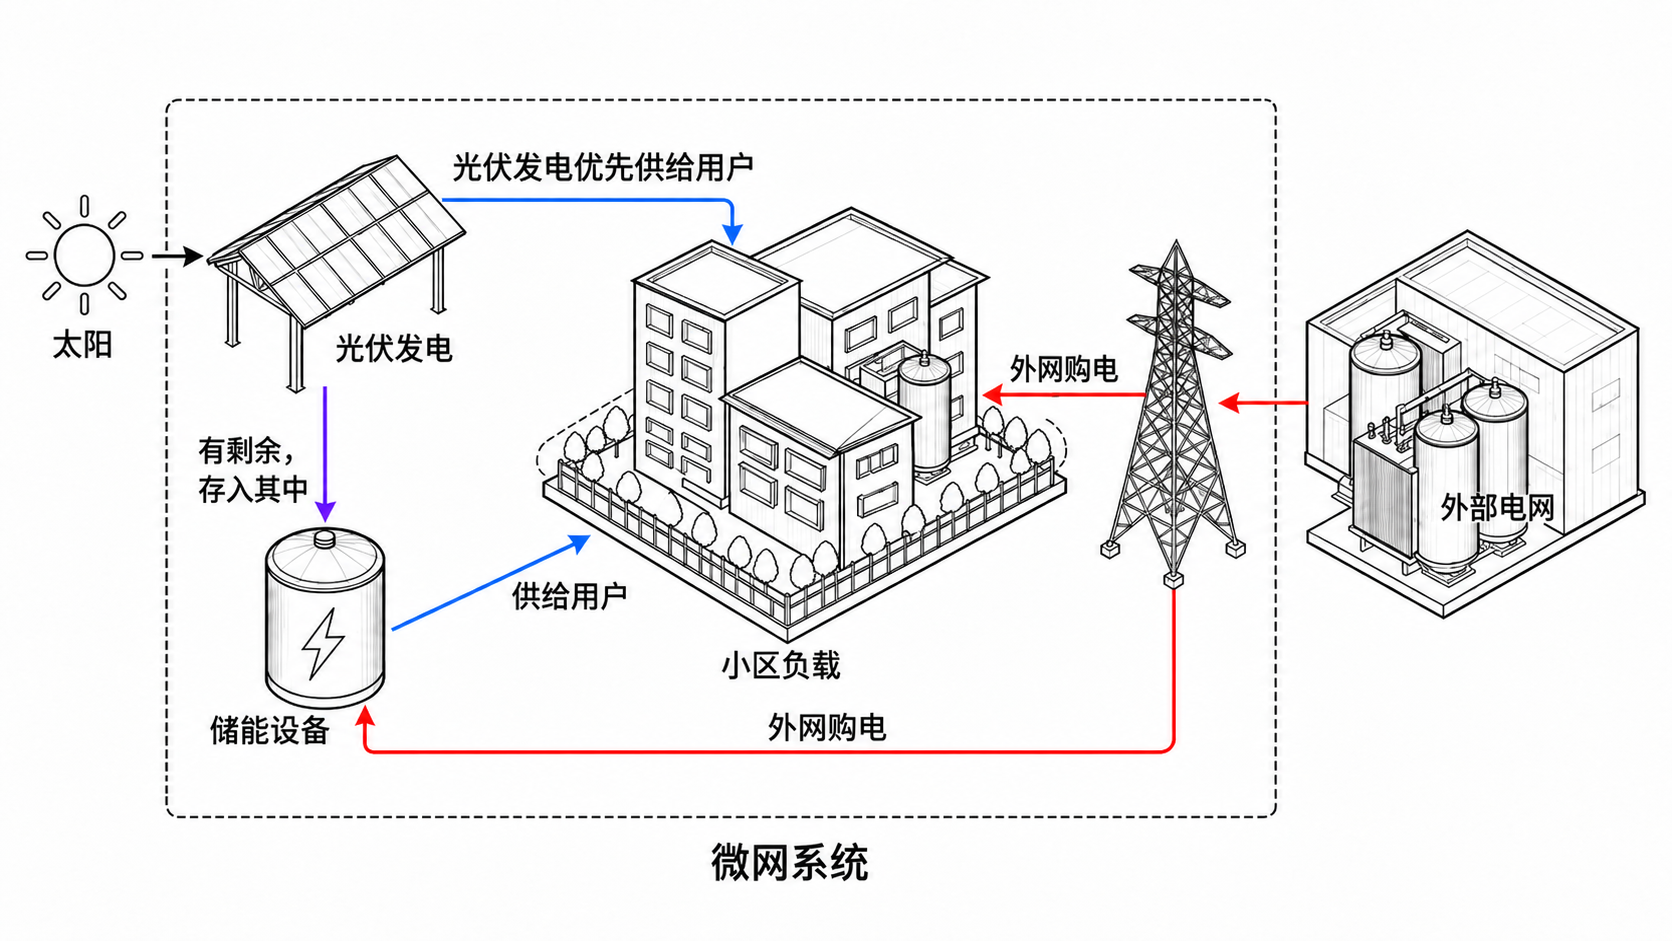
\includegraphics[width=0.9\textwidth]{fig/weiwang.png}
    \caption{微网系统流程图}
    \label{fig:weiwang}
\end{figure}

\subsection{问题提出}
\textbf{问题一：确定条件下的微网计划购电策略。}
已知一天内的负载、电价和光伏预测数据，制定当天的购电与储能充放电计划。
要求满足小区用电需求，并保证储能设备在 0:00 和 24:00 的电量相同，在此基础上尽量降低购电费用。

\textbf{问题二：实际供需变化下的每日购电。}
小区实际负载和光伏发电会随时间变化，因此每天都需要根据已有信息重新制定购电计划。
若实际供电不足，则需要按正常电价的 5 倍紧急购电，所以需要同时安排计划购电、储能使用和紧急购电，控制全年的总费用。

\textbf{问题三：利用更新的光伏预测调整购电计划。}
每天 0:00 先根据光伏预测制定计划，之后在 6:00、12:00 和 18:00 得到新的预测信息后，可以调整尚未执行的购电安排。
调整计划本身也会产生额外费用，因此需要比较“继续执行原计划”和“根据新预测进行调整”哪一种更划算，并判断是否有必要引入后续时刻的预测。

\textbf{问题四：波动电价下重新制定购电策略。}
进一步考虑外部电网电价随时间变化的情况，重新研究问题二和问题三中的购电与储能安排。
需要比较波动电价下的计划购电、储能使用、紧急购电和计划调整情况，并分析电价变化对微网购电策略和总费用的影响。
\section{问题分析}

四个问题围绕同一微网系统展开，核心都是在满足小区负载的前提下，协调光伏、外网购电和储能设备的使用。
随着问题推进，决策条件由“供需和价格已知”逐步扩展到“供需未知、预报更新以及电价波动”，因此建模过程也由确定性调度逐步转向预测与滚动优化。

\subsection{问题一的分析}

问题一属于\textbf{确定性优化问题}。题目已经给出一天内的负载、光伏预测和电价，因此本问不需要预测未来，重点是确定各时段何时购电、何时充电以及何时放电。

本问的主要难点是供需与价格存在明显的时间错位。白天可能出现光伏富余，而晚间仍有较大用电需求和较高电价。
若只根据当前电价独立决策，可能过早充满电池，无法继续接收后续光伏；也可能过早放电，导致真正高价时段缺少可用储能。
因此，需要同时考虑全天各时段，而不能逐时独立安排。

此外，题目要求0:00和24:00的储电量相同，从而避免通过消耗原有库存人为降低当天费用。
基于这些特点，本文将全天144个时段统一纳入\textbf{全时段电量流线性规划模型}，
在储能容量、充放电功率和效率等约束下，协调外网购电、光伏利用和储能转移，得到全天购电与充放电方案。

\subsection{问题二的分析}

问题二属于\textbf{预测与优化相结合的决策问题}。
与问题一不同，每天0:00制定计划时，当天真实负载和光伏尚未发生，因此不能直接使用附件中的未来实际数据，而必须根据此前已经发生的历史信息进行估计。

负载和光伏具有不同的变化特点：负载存在较明显的星期重复，而光伏更多受到近期发电水平变化的影响，因此二者分别预测，再合成为未来的净需求。

本问另一个关键困难是购电风险具有明显的不对称性。
普通电订多后即使没有使用，也需要付费；若订少导致供电不足，则需要按正常电价的5倍进行紧急购电。
储能虽然能够缓冲部分预测误差，但仍受到最低储电量和最大放电功率限制，因此不能仅靠电池解决全部偏差。

因此，本文采用\textbf{周期预测—近期加权准备—跨日线性规划}的思路：
先预测负载和光伏，再根据近期曾出现的净需求预测误差设置适量安全准备，最后利用线性规划安排普通购电和储能。
日末储电量直接传递到下一天，使各日运行连续衔接，而不是每天重新开始。

\subsection{问题三的分析}
问题三属于\textbf{动态信息下的滚动优化问题}。相比问题二，系统在6:00、12:00和18:00可以得到新的光伏预报，并允许调整尚未执行的购电计划。
问题的重点因此不只是“新预报是否更准确”，而是“利用新预报修改订单是否真正更经济”。

新的光伏预报可以修正零点时的判断，但改单本身需要支付额外费用；同时，如果电池仍有足够的调节空间，部分预测变化也可以直接由储能吸收。
因此，收到新预报并不意味着一定要修改订单，需要同时考虑：

\begin{itemize}
    \item 最新的负载和光伏判断；
    \item 当前真实储电量；
    \item 调增或调减订单的费用；
    \item 不调整后可能产生的紧急购电风险。
\end{itemize}

附件3给出的光伏预报为整点数据，而调度间隔为10分钟，因此需先将预报转换到统一时间尺度。
同时，官方预报能够反映当天最新信息，近期历史光伏则可以提供稳定参考，因此本文采用\textbf{历史融合预报—动态安全准备—日内滚动规划模型}。
每次获得新预报后，从当前真实储电状态重新优化未来尚未执行的部分，已经发生的时段保持不变。

此外，在评价日内预报价值时，需要区分“允许日内观察实际运行并修改订单”的作用和“新增光伏预报本身”的作用，避免把两类信息带来的收益混为一谈。

\subsection{问题四的分析}

问题四是在问题二、三的基础上进一步加入波动电价的不确定性。此时未来价格在决策时也尚未发生，因此不能简单沿用原来的购电方案，再用实际电价重新计算费用。因为电价变化本身会改变何时适合购电、何时应该充电以及储能应保留到哪个时段。

本问仍需分别对应问题二和问题三的两种决策权限。

对于问题四-2，每天只能在0:00确定普通购电计划，无法利用当天已经发生的价格进行修正，因此需要从历史价格、星期位置、季节特征和预测净负荷中判断未来价格。
考虑到这些因素与价格之间可能存在非线性关系，采用\textbf{滚动提升树—零点线性规划模型}。

对于问题四-3，6:00、12:00和18:00可以利用当天已经发生的价格更新后续判断。
由于历史价格特征之间相关性较强，同时需要保持日内多次修正的稳定性和可解释性，
因此采用\textbf{滚动岭回归—日内调整线性规划模型}。预测价格只作为购电和储能优化的决策依据，最终费用仍按照真实发生的电价结算。
\section{模型假设与符号说明}

\subsection{模型假设}

在题目给定的设备参数和交易规则基础上，为统一四个问题中的电量流向、时间尺度和信息使用范围，作如下假设。

\begin{enumerate}
    \item \textbf{光伏优先直接满足小区负载。}
    当光伏功率超过当前负载时，富余部分可用于储能；外网购电既可直接供给负载，也可用于给储能设备充电。题目未给出售电规则，因此未被负载或储能利用的光伏不计售电收益。

    \item \textbf{以10分钟为一个调度时段。}
    认为每个采样点的负载功率、光伏功率和电价在其对应的10分钟区间内保持不变，并据此将功率转换为区间电量。该离散化与题目要求的10分钟购电结果保持一致。

    \item \textbf{储电状态按时间连续衔接。}
    问题一按照题意要求日初和日末储电量相等；问题二至问题四则将前一天24:00的实际剩余电量作为下一天0:00的初始电量，不再每日重置储能状态。

    \item \textbf{决策只使用当时已经获得的信息。}
    问题二制定零点计划时，只使用此前已经发生的负载、光伏和储电状态；问题三只使用对应时刻已经发布的光伏预报；问题四中未来实际电价同样不能提前使用。由此避免在模型中引入未来信息。

    \item \textbf{订单调整以零点原计划为统一基准。}
    在问题三及问题四的日内调整分支中，已经执行的订单不再修改；同一时段经过多次调整时，只计算最终订单相对零点原计划的净变化，避免重复计算调整费用。

    \item \textbf{不额外考虑题目未给出的储能损耗因素。}
    除题目规定的充、放电效率外，不再引入电池自放电、寿命折旧等额外成本。这样既避免人为增加缺乏参数支持的费用项，也使目标函数集中于题目要求的购电成本。

\end{enumerate}


\subsection{符号说明}

设 $d$ 表示日期，$k$ 表示一天中的第 $k$ 个10分钟时段，其中

\begin{equation}
k=1,2,\ldots,144,
\qquad
\Delta t=\frac{1}{6}\ \mathrm{h}.
\end{equation}

$S_{d,0}$ 表示第 $d$ 天0:00的储电量，$S_{d,k}$ 表示第 $k$ 个时段结束后的储电量。问题一仅研究一个代表日，因此相应公式中可省略日期下标 $d$。

主要公共符号如表所示。各问中特有的预测误差、准备量、订单调整量及价格模型参数，在对应模型中首次出现时再单独定义。

\begin{table}[H]
    \centering
    \caption{主要符号及其含义}
    \begin{tabular}{ccl}
        \hline
        符号 & 含义 & 单位或取值 \\
        \hline
        $d$ & 日期下标 & -- \\
        $k$ & 日内10分钟时段下标 & $1,\ldots,144$ \\
        $\Delta t$ & 单个调度时段长度 & $1/6\,\mathrm{h}$ \\
        $L_{d,k}$ & 小区负载功率 & kW \\
        $P^{PV}_{d,k}$ & 光伏发电功率 & kW \\
        $E^L_{d,k}$ & 第 $k$ 时段负载电量 & kWh \\
        $E^{PV}_{d,k}$ & 第 $k$ 时段光伏电量 & kWh \\
        $p_{d,k}$ & 对应时段外网电价 & 元/kWh \\
        $m_{d,k}$ & 光伏直接供给负载的电量 & kWh \\
        $n_{d,k}$ & 光伏直供后的负载缺口 & kWh \\
        $r_{d,k}$ & 光伏直供后的富余电量 & kWh \\
        $q_{d,k}$ & 普通外网购电量 & kWh \\
        $x_{d,k}$ & 外网购电中用于储能充电的电量 & kWh \\
        $y_{d,k}$ & 富余光伏用于储能充电的电量 & kWh \\
        $z_{d,k}$ & 储能设备向负载输出的电量 & kWh \\
        $S_{d,k}$ & 第 $k$ 时段结束后的内部储电量 & kWh \\
        $w_{d,k}$ & 未被负载或储能利用的光伏电量 & kWh \\
        $S_{\min}$ & 储电量运行下限 & 1200 kWh \\
        $S_{\max}$ & 储电量运行上限 & 10800 kWh \\
        $P_{\max}$ & 最大充、放电功率 & 5000 kW \\
        $\eta_c$ & 充电效率 & 0.90 \\
        $\eta_d$ & 放电效率 & 0.90 \\
        \hline
    \end{tabular}
\end{table}

上述符号构成四个问题共用的电量流和储能状态基础，其中设备容量、功率和效率均直接采用题目给定参数，而非额外假设。
\section{数据预处理与探索性分析}

\subsection{数据预处理}
本文数据均来自赛题附件。
附件1提供代表日的电价、负载和光伏预测数据；附件2提供2025年全年实际负载和光伏功率；
附件3提供每日多时刻发布的光伏预测；附件4提供全年实际电价。
我们对这些数据进行了\textbf{清洗、格式统一、结构整理和模型所需转换}，确保后续建模与求解的准确性，具体操作如下：

\begin{enumerate}
\item \textbf{数据质量检查。}
首先检查附件1—4中的缺失值、非数值项、异常取值及时间对应关系。
核查后，原表已有记录中不存在需要填补的空值。光伏零值主要对应夜间无发电情况，因此予以保留；较大或较小的负载、光伏和电价值经原始附件核对后也不作删除。需要区分的是，按真实区间起点建立全年时间轴后，1月1日00:00--00:10缺少实际观测，其启动处理在问题二中单独说明，不作为原始实测数据补入。

\item \textbf{时间与数据格式统一。}
统一日期和时间格式，并按照“日期—时间”建立负载、光伏和电价之间的对应关系。
针对“0:00+1”等特殊时间标签，按照其真实时间含义进行映射，避免数据错位。对于光伏预报，同时保留预报发布时间和目标时刻，不同发布时间的预报不相互覆盖。
下文日均、月均功率按原表日期与采样标签分组，末行次日零点随原标签参与描述统计；调度计算则按实际区间起点排序，全年序列中的次日零点归入次日，问题一的周期零点单独对应首段。

\item \textbf{数据结构整理。}
将原始宽表整理为逐时记录形式，便于不同附件按相同时刻进行匹配。
该过程只改变数据排列方式，不增加、删除或修改原始观测值。对于超出实测时间范围的预报，仅在误差计算时不参与比较，原始预报仍予以保留。

\item \textbf{模型所需转换与核对。}
后续调度以10分钟为一个时段。负载和光伏的功率数据在模型中按
\begin{equation}
E = P \times \frac{1}{6}
\end{equation}
转换为相应时段电量。供需平衡和储能调度保留各变量的物理单位，不对这些物理量作归一化；价格回归所需的特征标准化在问题四中单独进行。整理后的观测值与原始附件逐项核对，确保数值及对应关系一致。
\end{enumerate}


\subsection{探索性分析}
在完成了数据的预处理与分析之后，我们对数据有以下发现：

\subsubsection*{（1）光伏富余与用电需求存在明显的时间错位}
根据附件1的代表日数据，我们对负载、光伏功率和电价进行日内对比，结果如图\ref{fig:tsxfx_1}所示。

\begin{figure}[H]
    \centering
    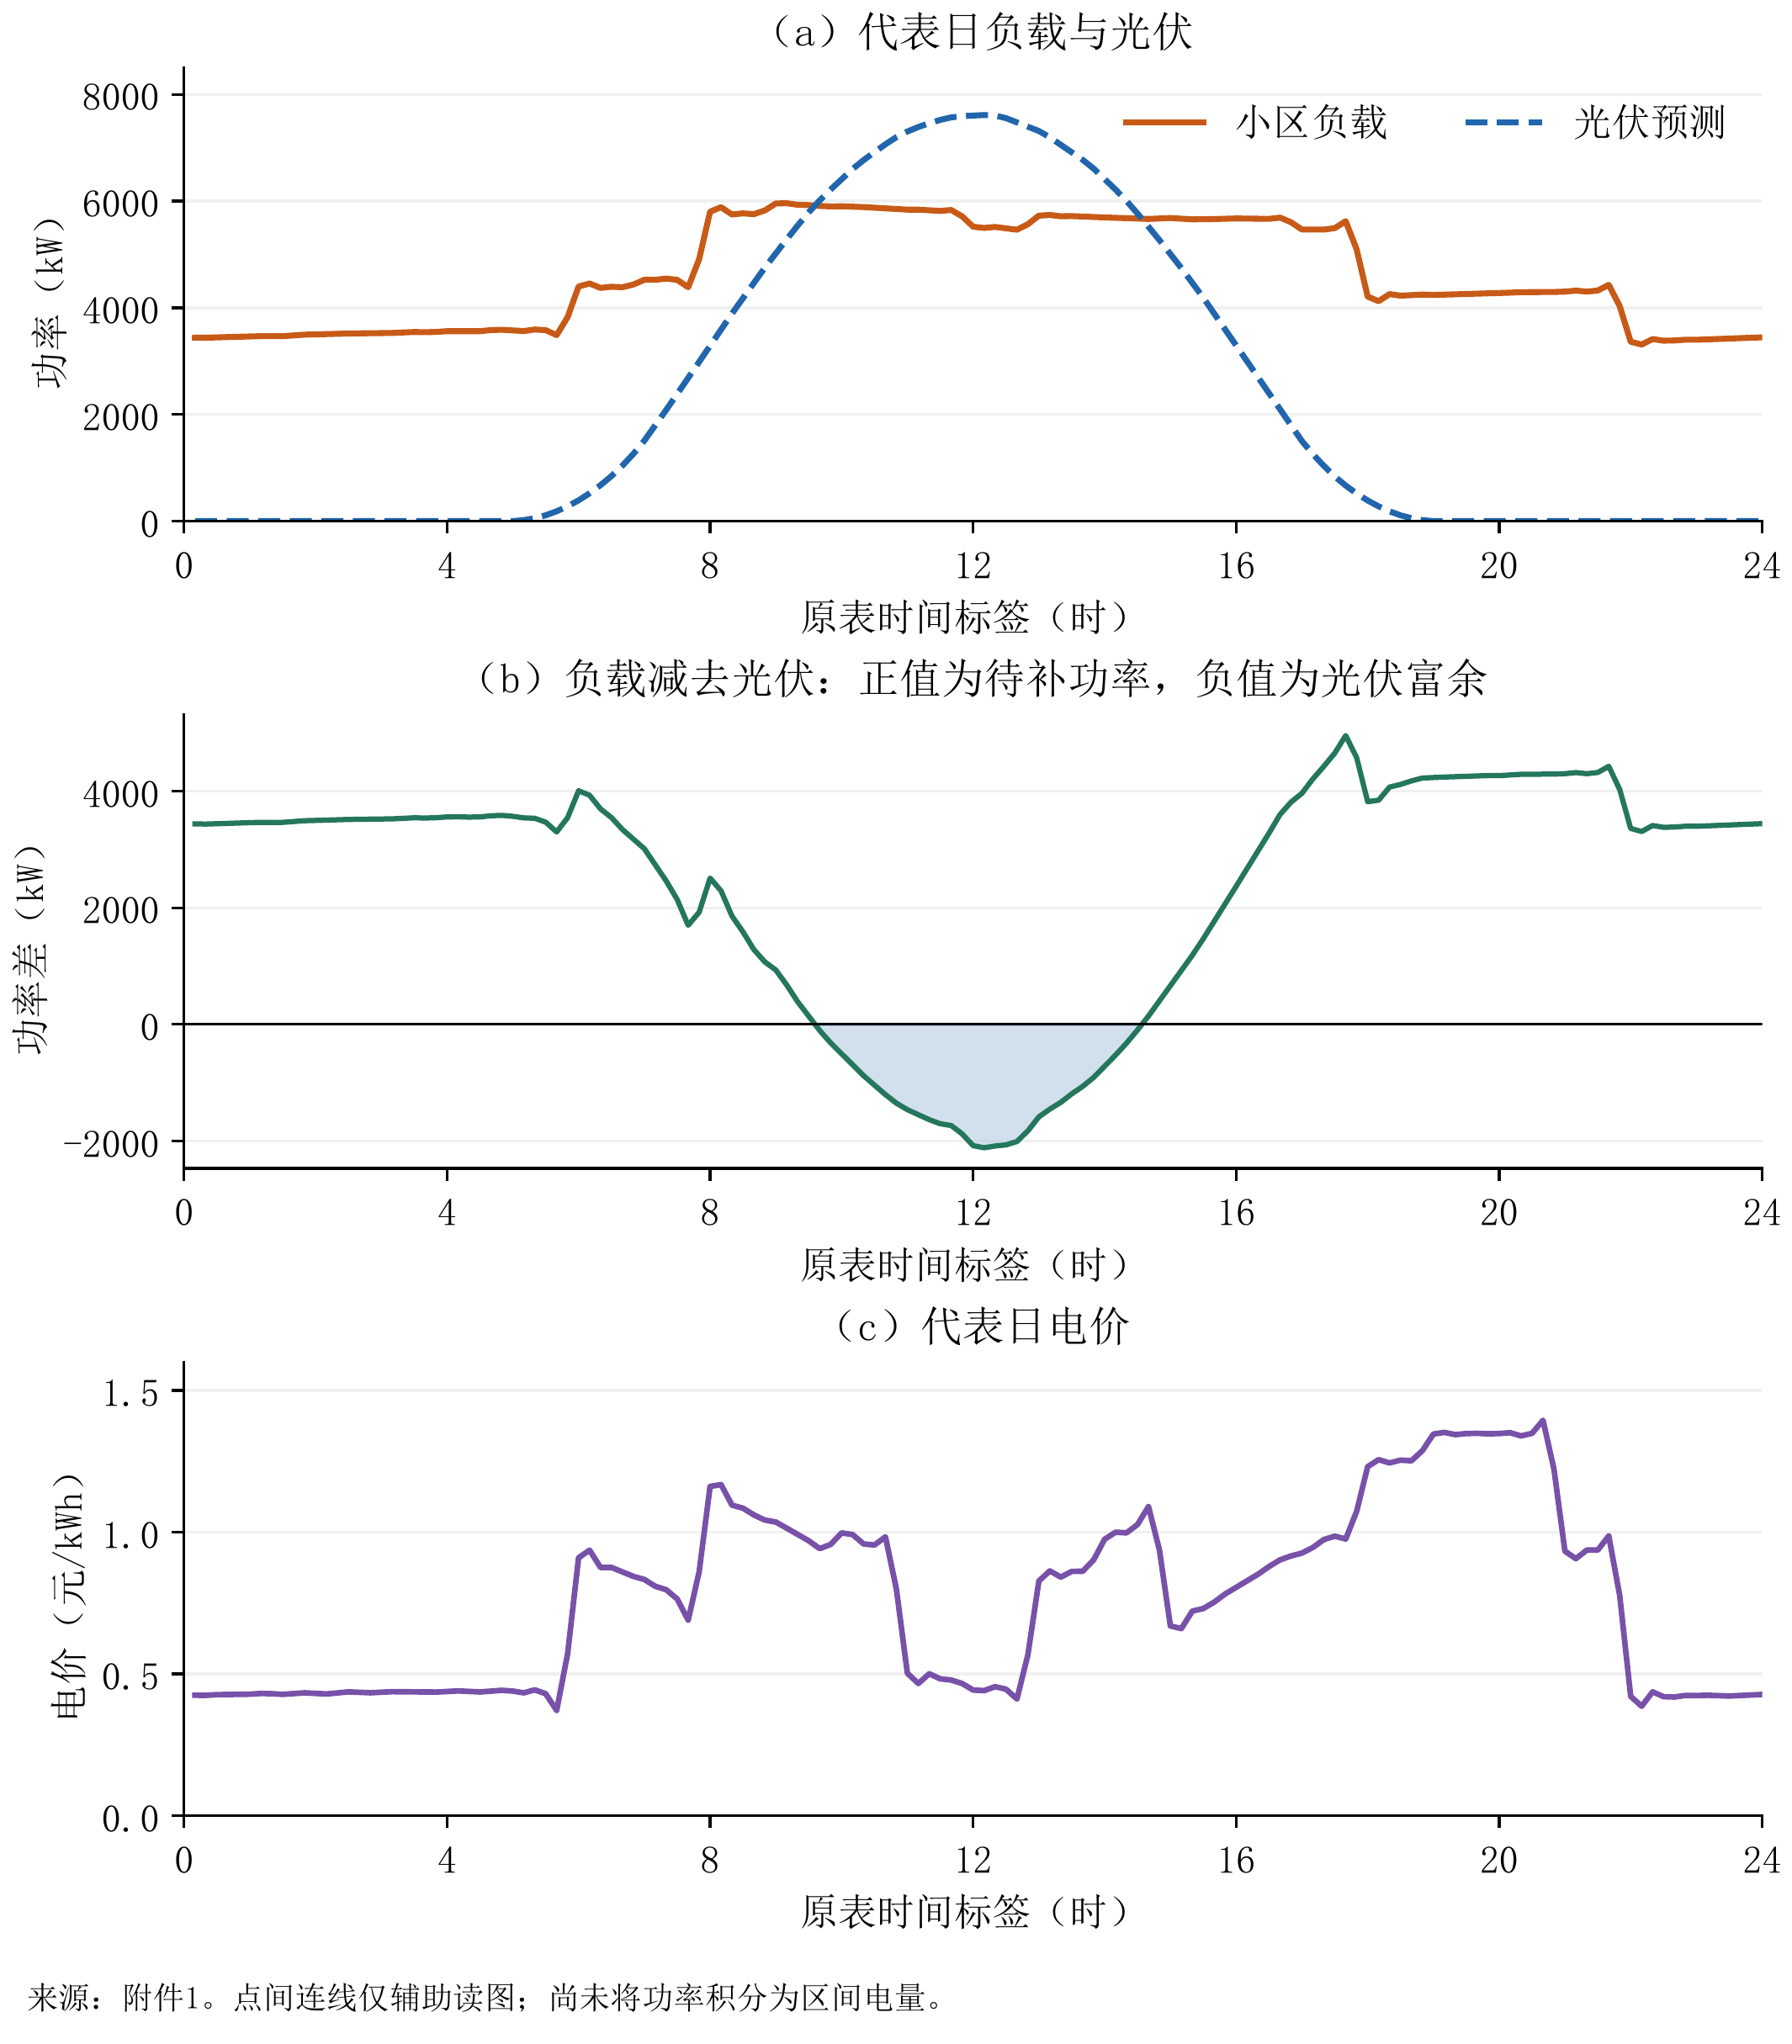
\includegraphics[width=0.8\textwidth]{fig/tsxfx_1.png}
    \caption{代表日供需与电价的时间错配}
    \label{fig:tsxfx_1}
\end{figure}

由图\ref{fig:tsxfx_1}(a)可见，光伏功率主要在白天上升，并在午间达到较高水平，而小区负载全天均保持在较高水平。
进一步由图\ref{fig:tsxfx_1}(b)可见，午间“负载减光伏”为负，说明此时存在光伏富余；进入傍晚后，光伏快速下降，供需缺口重新扩大。
代表日午间最大光伏富余功率约为 \(2100\,\mathrm{kW}\)，而傍晚最大供需缺口接近 \(5000\,\mathrm{kW}\)。

同时，图\ref{fig:tsxfx_1}(c)表明较高电价主要出现在傍晚和晚间，与较大的供需缺口具有一定重合。这意味着高需求时段往往也是购电成本较高的时段。

进一步统计全年数据发现，共有330天出现过光伏功率高于负载的情况，说明午间光伏富余并非个别现象。

因此，\textbf{光伏发电充足的时段与主要用电时段并不一致}。仅比较全天总发电量和总负载无法反映真实运行压力。
储能需要承担跨时段转移电量的作用，将午间富余光伏或低价购电转移到后续高需求、高电价时段使用。


\subsubsection*{（2）负载和光伏均存在年内变化，但变化并不同步}
根据附件2和附件4，我们对全年负载、光伏和电价分别计算每日平均值和月平均值，结果如图\ref{fig:tsxfx_2}所示。

\begin{figure}[H]
    \centering
    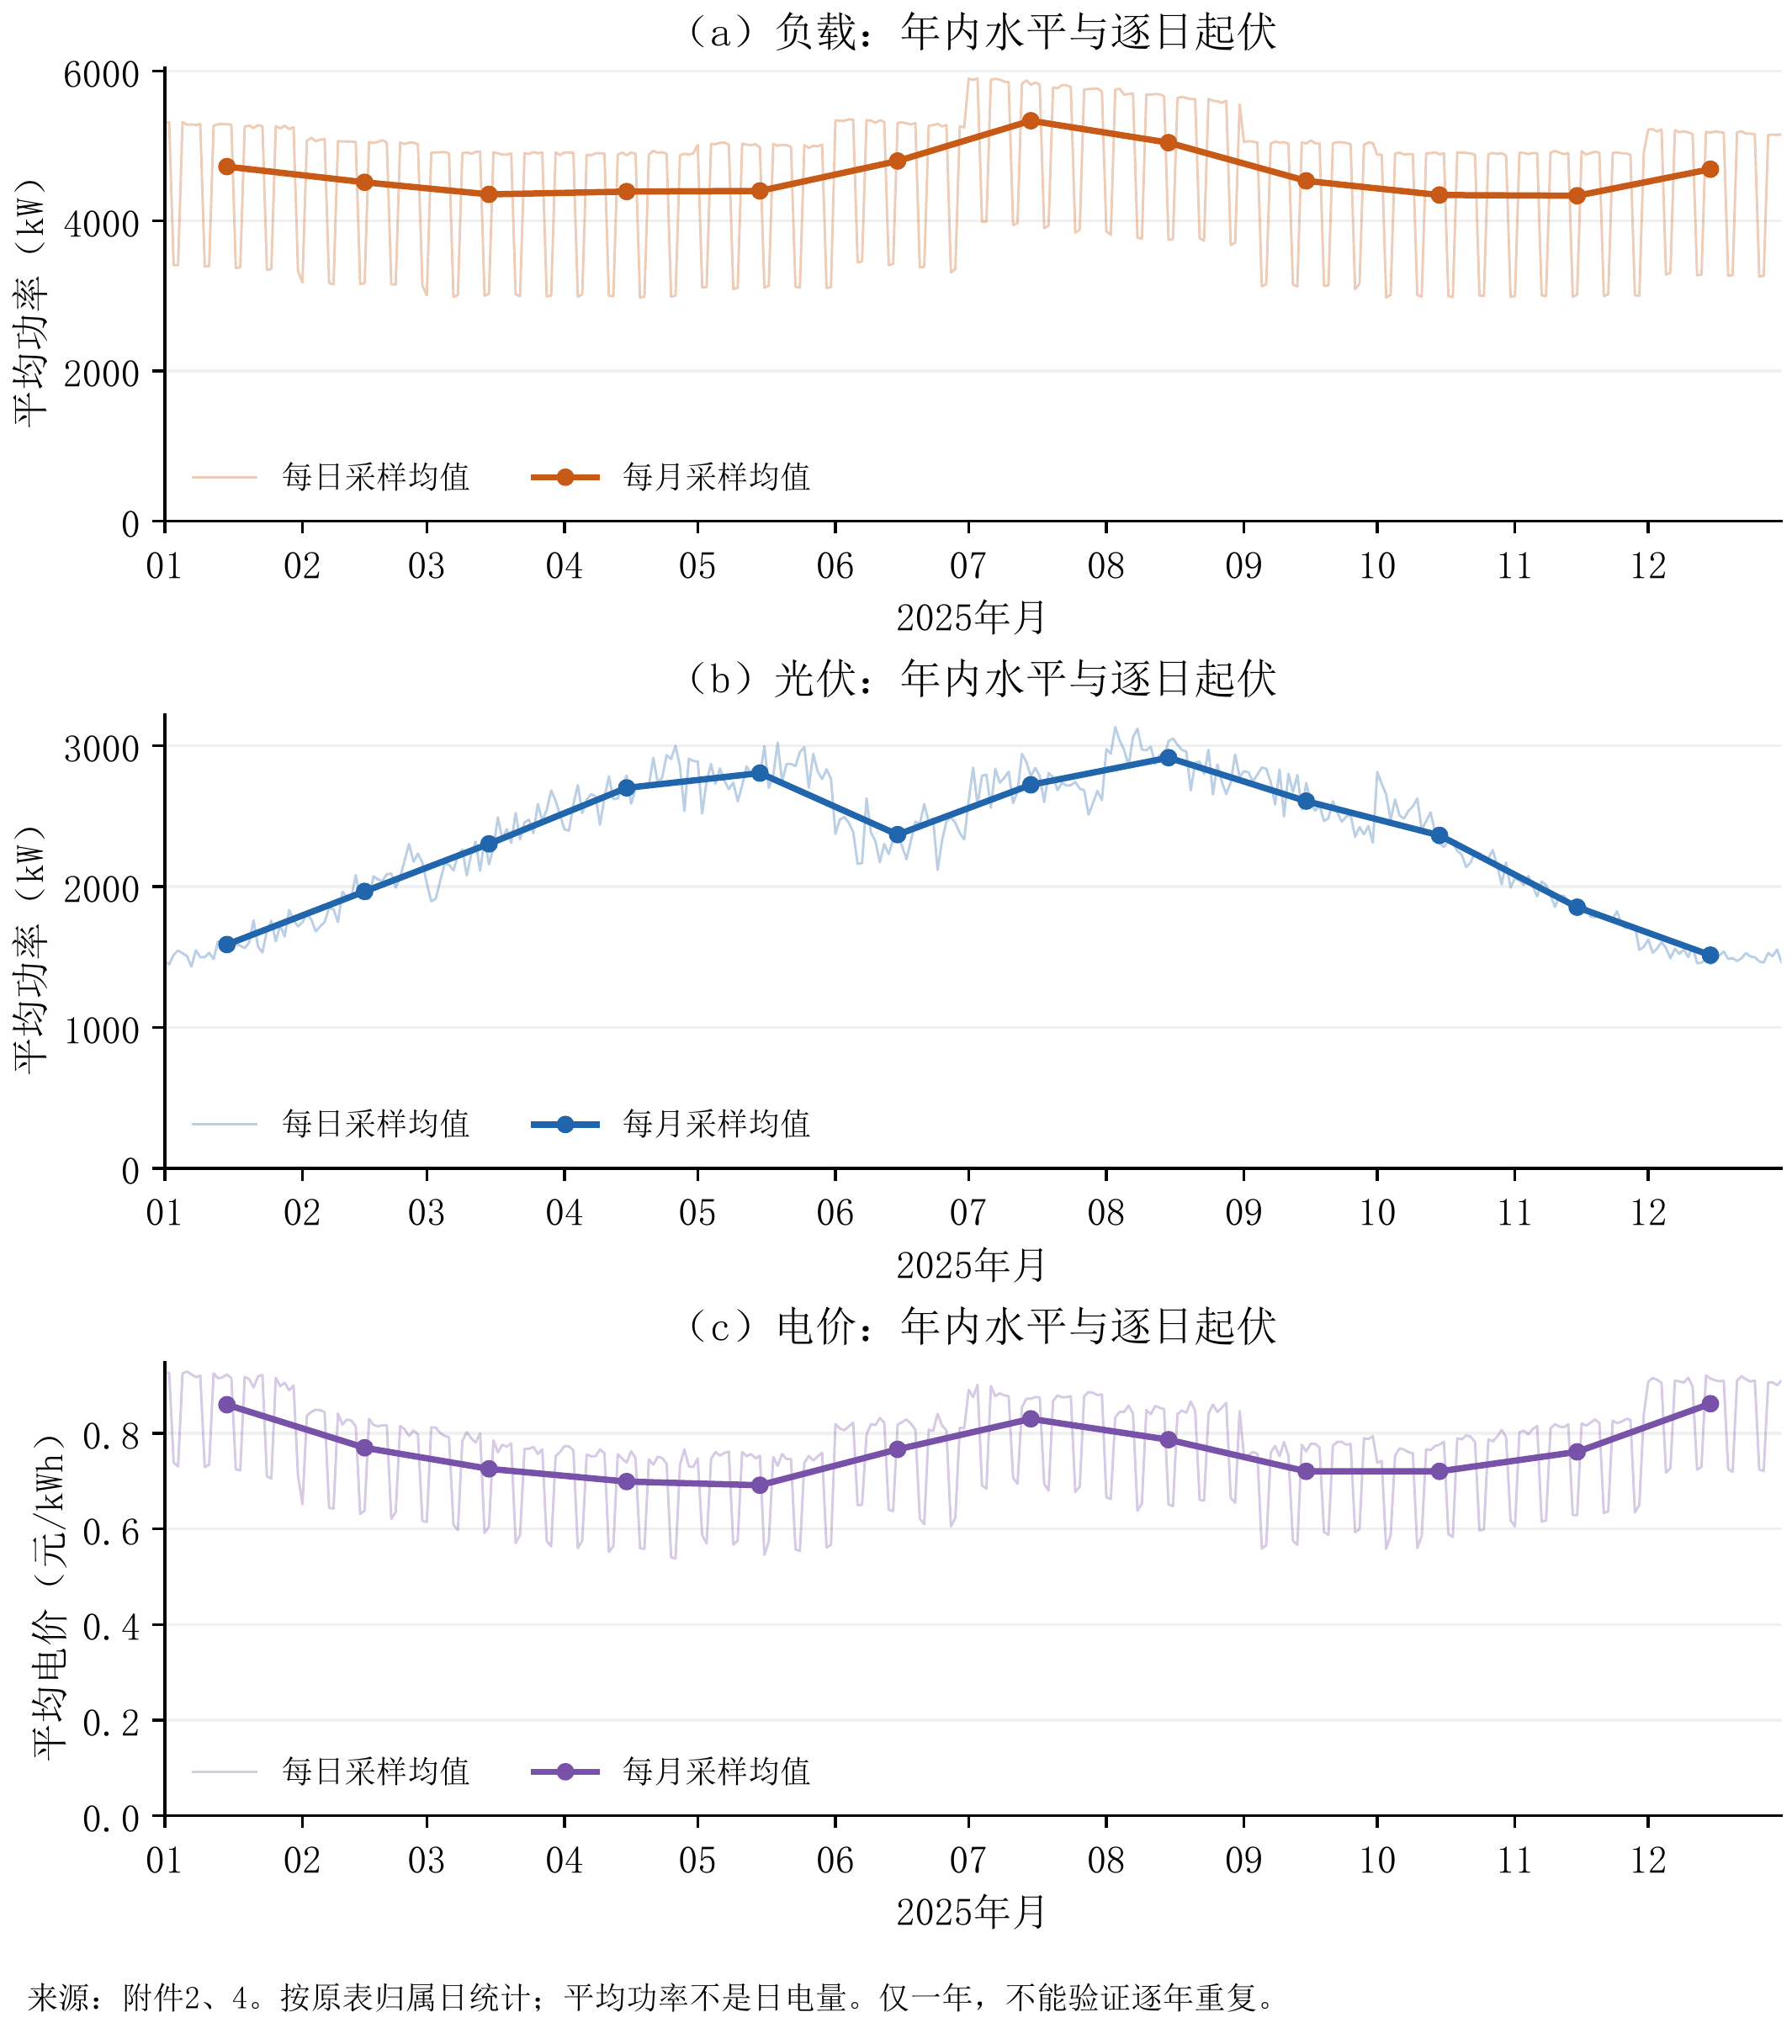
\includegraphics[width=0.8\textwidth]{fig/tsxfx_2.png}
    \caption{代表日供需与电价的时间错配}
    \label{fig:tsxfx_2}
\end{figure}

由图\ref{fig:tsxfx_2}(a)可见，小区负载存在明显的年内变化，夏季整体水平较高；
图\ref{fig:tsxfx_2}(b)显示光伏同样具有季节变化，但其变化趋势与负载并不完全一致。特别是在冬季，负载虽然低于夏季高峰，但光伏出力下降更加明显。

例如，12月平均负载减去光伏后的功率差约为 \(3177\,\mathrm{kW}\)，而5月约为 \(1595\,\mathrm{kW}\)，前者接近后者的两倍。

这说明，\textbf{外网补电压力并不能仅由负载高低决定，还必须同时考虑光伏出力}。
夏季负载虽然较高，但光伏也能提供较多电量；冬季负载并非最高，但由于光伏下降，实际供需缺口仍可能较大。

图\ref{fig:tsxfx_2}(c)还表明全年平均电价同样存在一定的年内起伏。因此，不同月份面临的供需条件和购电环境均有差异，不能将某一天或某一固定购电、充放电策略直接复制到全年。


\subsubsection*{（3）负载具有明显的周重复特征，电价存在跨日波动}
为进一步分析日际规律，我们按实际星期对全年负载和电价进行分组，结果如图\ref{fig:tsxfx_3}所示。

\begin{figure}[H]
    \centering
    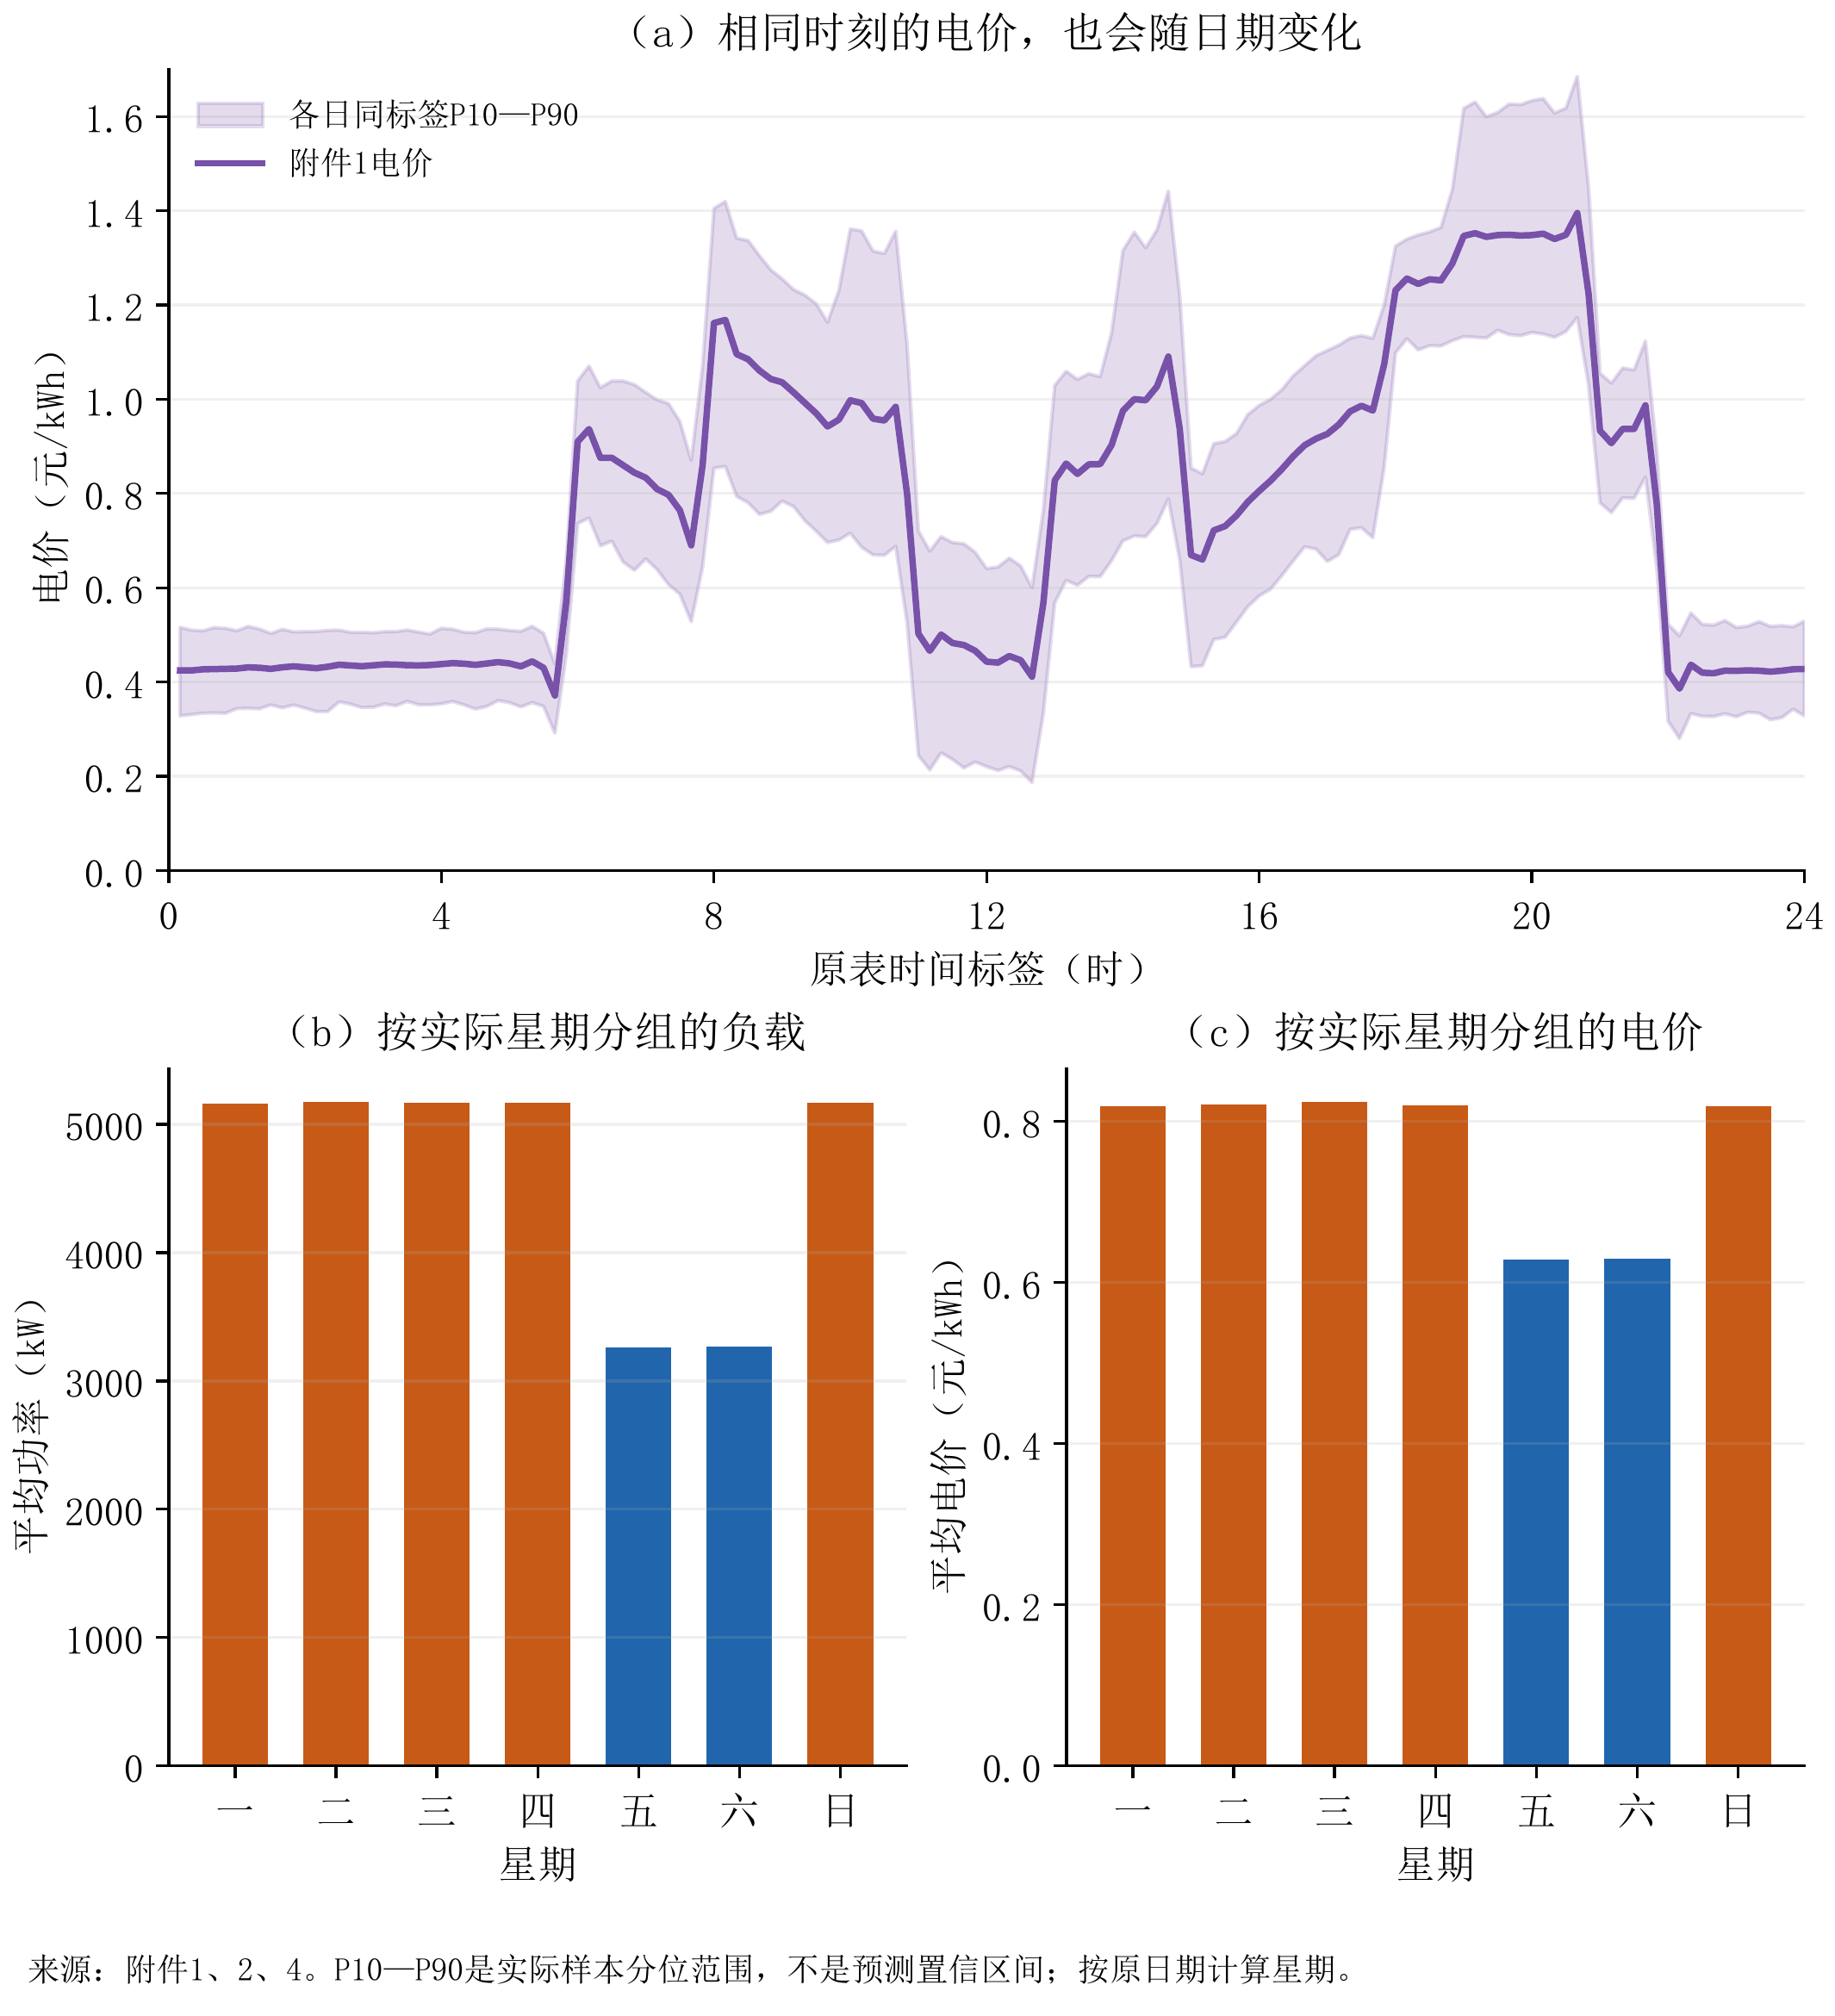
\includegraphics[width=0.8\textwidth]{fig/tsxfx_3.png}
    \caption{代表日供需与电价的时间错配}
    \label{fig:tsxfx_3}
\end{figure}

由图\ref{fig:tsxfx_3}(b)可见，周五和周六的平均负载明显低于其他日期。
统计结果显示，周五和周六的平均负载约为 \(3265\,\mathrm{kW}\)，其余五天约为 \(5168\,\mathrm{kW}\)，前者低约 \(36.8\%\)。
同时，负载与一周前数据的相关性明显高于与前一天数据的相关性，说明负载具有较强的周重复特征。

因此，在利用历史信息判断未来负载时，\textbf{同一星期位置的历史数据具有较强参考价值}，不能只根据前一天的数据进行简单外推。
    
光伏则表现不同。虽然始光伏序列在不同日期之间具有较高相似性，但在扣除各月相同时刻的平均日内轮廓后，其一周相关性接近于零。
这说明光伏曲线的相似主要来自“白天高、夜间低”的共同日内形状，而不是稳定的星期周期。

另一方面，图\ref{fig:tsxfx_3}(a)给出了全年相同时刻电价的第10至第90百分位范围。可以看到，即使处于相同的日内时刻，不同日期的实际电价仍存在明显差异。
图\ref{fig:tsxfx_3}(c)虽然显示不同星期的平均电价存在一定规律，但历史低价时段并不能保证未来同一时刻仍保持相同价格。

因此，\textbf{负载、光伏和电价的历史规律并不完全相同}。负载可以更多参考周重复信息，而光伏和电价仍需考虑较强的日际变化。  


\subsubsection*{（4）日内更新能够提高光伏预报精度，但并非每次更新都更准确}
根据附件3，我们将不同发布时间的光伏预报与相同目标时刻的实际光伏进行匹配，并采用平均绝对误差评价预测偏差，结果如图\ref{fig:tsxfx_4}所示。

\begin{figure}[H]
    \centering
    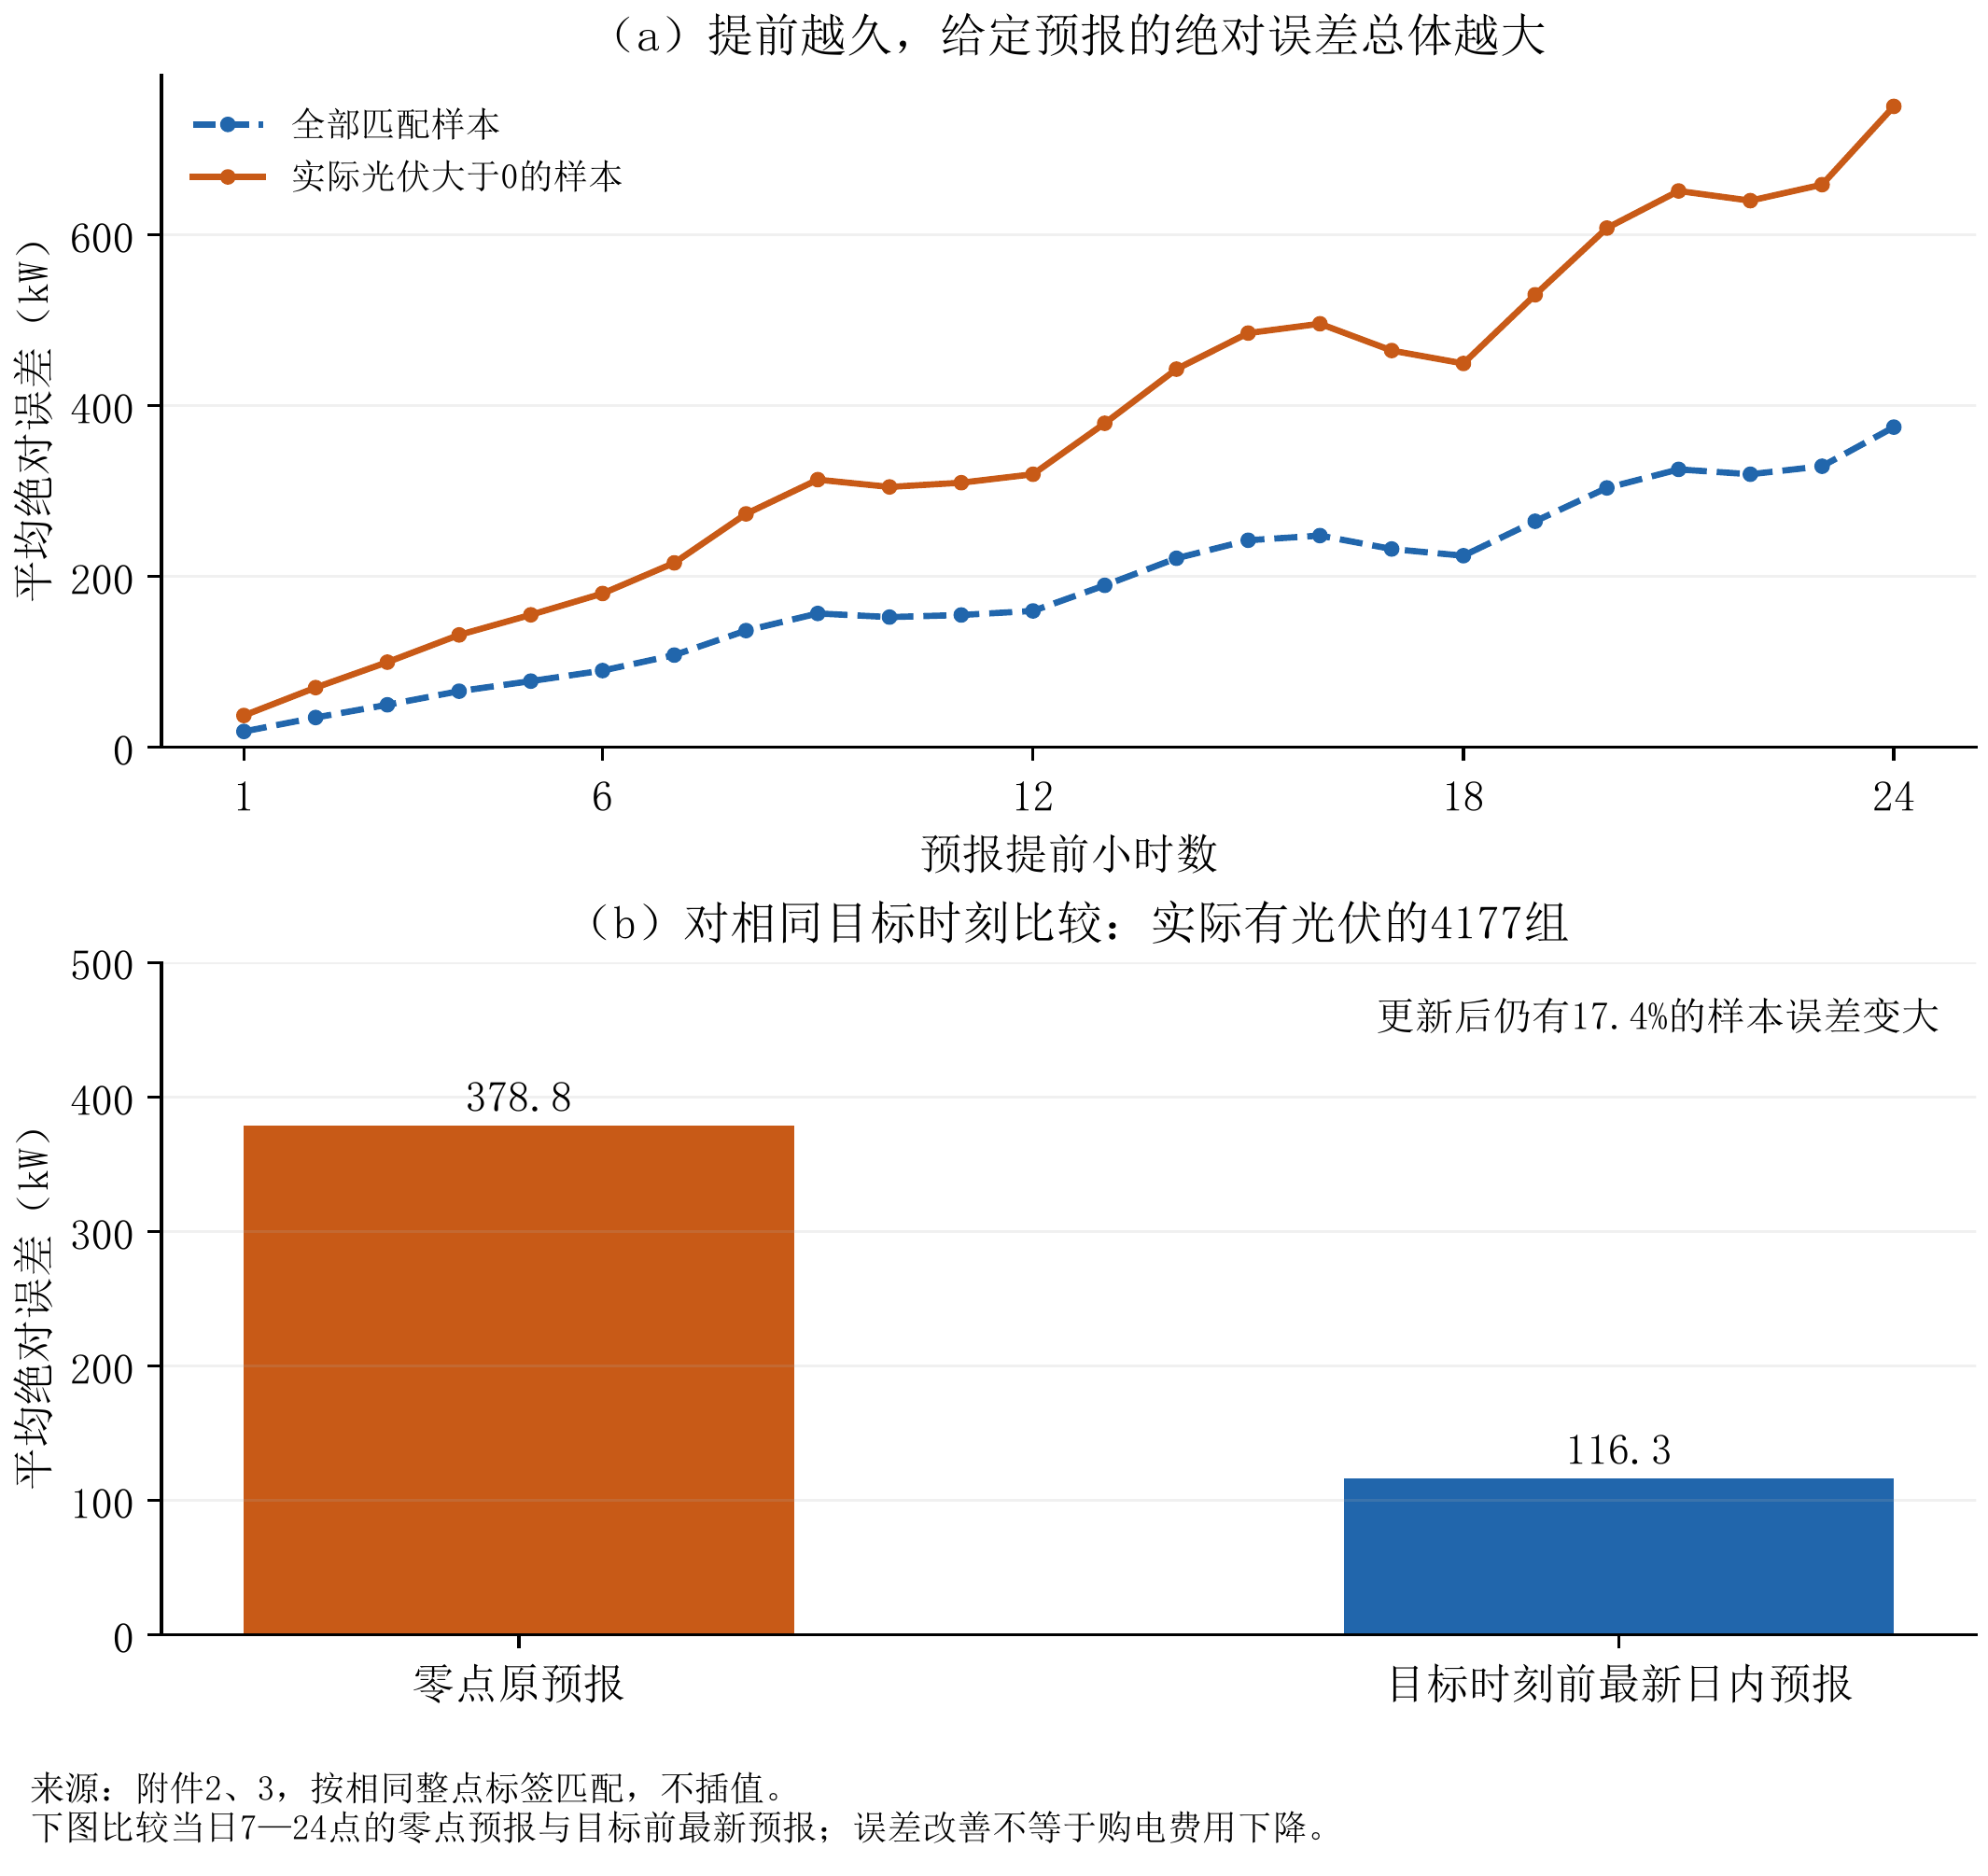
\includegraphics[width=0.8\textwidth]{fig/tsxfx_4.png}
    \caption{代表日供需与电价的时间错配}
    \label{fig:tsxfx_4}
\end{figure}

由图\ref{fig:tsxfx_4}(a)可以看出，随着预报提前时间增加，平均绝对误差总体呈上升趋势，说明距离目标时刻越远，光伏预报通常越不准确。特别是在实际存在光伏出力的样本中，误差更加明显。

为了进一步判断日内更新是否有效，图\ref{fig:tsxfx_4}(b)比较了同一目标时刻下的零点原预报和目标时刻前最新日内预报。
在实际光伏大于0的4177组样本中，平均绝对误差由约 \(378.8\,\mathrm{kW}\) 降低至 \(116.3\,\mathrm{kW}\)，下降约 \(69\%\)。这说明日内更新总体上明显提高了预报精度。

但图\ref{fig:tsxfx_4}(b)同时显示，仍有约 \(17.4\%\) 的样本在更新后误差反而增大。因此，新的预报虽然总体更准确，但\textbf{并不意味着每次更新都一定优于原预报}。

此外，预测误差降低也不等于购电费用按相同比例降低。如果新的预测偏差可以由储能设备自行吸收，则调整购电计划未必划算；
只有当更新后的预测明显改变未来供需缺口，并且节省的紧急购电费用能够覆盖调整成本时，日内预报更新才具有实际经济价值。

\section{问题一的模型建立与求解}

%====================
\subsection{求解思路与模型选择}

问题一已知一天内各时段的负载、光伏预测和电价，需要确定外网购电量以及储能设备的充放电安排，在满足负载需求和储能运行约束的前提下，使全天购电费用尽可能低。
同时，题目要求0:00与24:00的储电量相同。

由前文探索性分析可知，午间容易出现光伏富余，而较大的供需缺口和较高电价更多出现在傍晚。
因此，当前时段是否充放电，会直接影响后续可使用的储能。若仅采用“低价充电、高价放电”的简单规则，可能过早充满或放空电池，错过后续更有价值的调节时机。

基于这一特点，本文首先考虑两种较直观的调度思路作为对照。
第一种为\textbf{峰谷电价策略}，按照“低价充电、高价放电”的原则，根据电价门槛安排储能；
第二种为\textbf{光伏空间预留策略}，在峰谷电价策略基础上，结合午间光伏富余的特点，为后续光伏预留一定储能空间。

这两种规则策略能够反映较直观的调度思路，但都需要事先设定价格门槛或目标储电量，难以同时考虑当前充放电行为对后续高价时段和光伏富余时段的影响。
为此，本文进一步将全天144个10分钟时段统一考虑，同时优化各时段的购电、充电和放电安排。

由于购电费用、供需平衡、储电量变化以及容量和充放电功率约束均可表示为线性关系，因此建立\textbf{线性规划模型}。
后续在相同的代表日数据、充放电效率和首尾储电量条件下，将线性规划与上述两种规则策略进行比较，并根据实际购电费用确定最终采用的方案。

%====================
\subsection{问题一的模型建立}

\subsubsection*{（1）时段与电量划分}

将一天划分为144个10分钟时段，记为
\[
k=1,2,\ldots,144,\qquad \Delta t=\frac{1}{6}\text{ h}.
\]
各时段采用起点采样值代表该区间内的功率和电价。例如，00:10的记录对应00:10--00:20。附件1描述每日重复的代表日，末行零点记录对应首段00:00--00:10，其余记录按实际时刻对应区间，不直接以表格行号确定时段。

第 \(k\) 个时段的负载电量和光伏电量分别为
\begin{equation}
E_k^L=L_k\Delta t,\qquad
E_k^{PV}=P_k^{PV}\Delta t.
\label{eq:q1_energy}
\end{equation}

按照“光伏优先满足负载”的原则，定义光伏直接供给负载的电量为
\[
m_k=\min(E_k^L,E_k^{PV}),
\]
进一步得到光伏直供后的负载缺口和光伏富余量：
\begin{equation}
n_k=E_k^L-m_k,\qquad
r_k=E_k^{PV}-m_k.
\label{eq:q1_gap_surplus}
\end{equation}

其中，\(n_k\) 表示该时段仍需由外网或储能补充的电量，\(r_k\) 表示可用于储能的富余光伏。

\subsubsection*{（2）决策变量与电量流向}

设
\[
x_k:\text{外网用于储能充电的电量},
\]
\[
y_k:\text{富余光伏用于储能充电的电量},
\]
\[
z_k:\text{储能向负载放出的电量},
\]
\[
S_k:\text{第 }k\text{ 时段结束时的储电量}.
\]
上述变量均以kWh计量，其中$x_k$、$y_k$和$z_k$按储能设备外侧计量，$S_k$按电池内部计量。这样，充放电量与内部储电量通过充、放电效率联系起来，避免将进入设备的电量直接等同于实际存入的电量。

各类电量之间的关系如图~\ref{fig:q1_1}所示。光伏优先直接满足负载，富余部分可用于储能；外部电网既可直接补足负载，也可为储能充电；储能则在需要时向负载放电。

\begin{figure}[H]
    \centering
    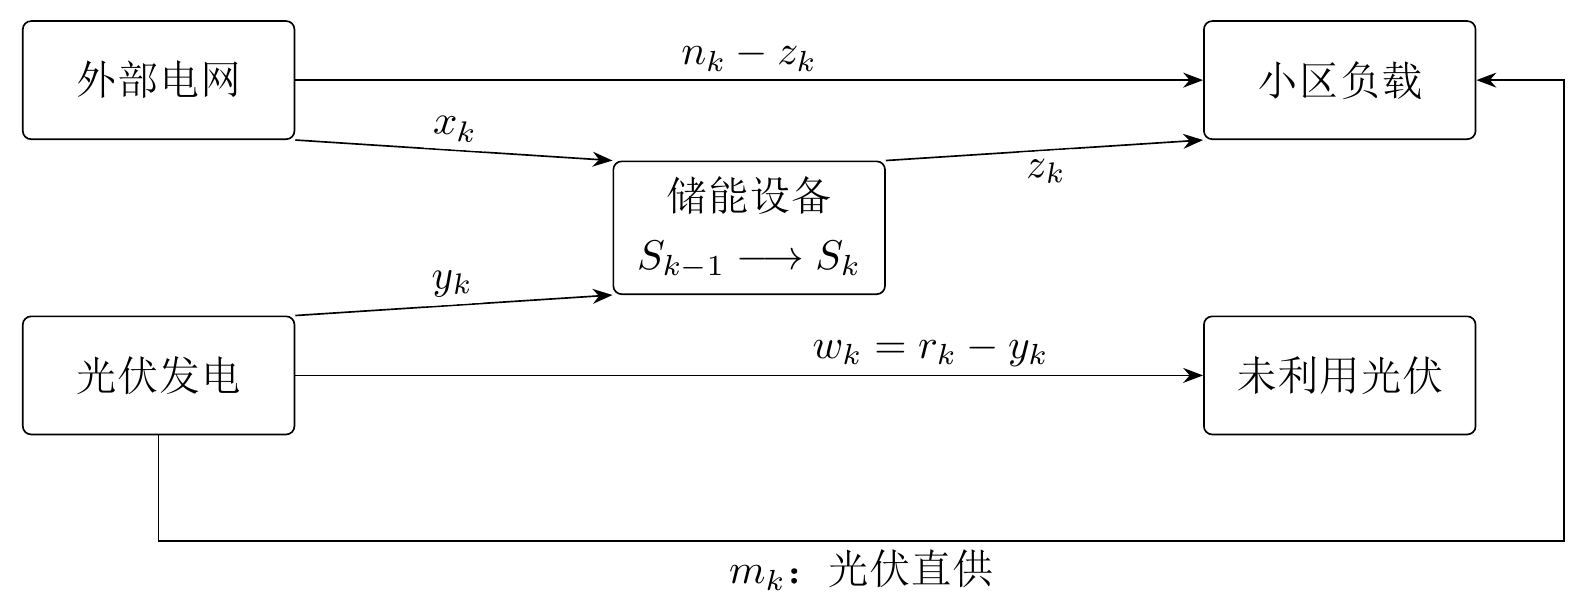
\includegraphics[width=0.95\textwidth]{fig/q1_1.png}
    \caption{问题一的电量分配关系}
    \label{fig:q1_1}
\end{figure}

因此，第 \(k\) 个时段的外网购电量为
\begin{equation}
q_k=n_k-z_k+x_k.
\label{eq:q1_purchase}
\end{equation}

未被利用的光伏量为
\[
w_k=r_k-y_k.
\]

\subsubsection*{（3）目标函数}

问题一只计算外网购电费用，因此以全天购电费用最小为目标：
\begin{equation}
\min C=
\sum_{k=1}^{144}
p_k\left(n_k-z_k+x_k\right),
\label{eq:q1_objective}
\end{equation}
其中，\(p_k\) 为第 \(k\) 个时段的电价。

该目标最小化的是\textbf{购电费用，而不是购电总量}。因此，模型允许在低价时段适当多购电，并通过储能减少后续高价时段的购电。

\subsubsection*{（4）约束条件}

为保证购电与储能调度方案能够实际执行，模型需同时满足供需平衡、充放电功率、储电容量以及日首尾储电量约束。

\textbf{1）供需与光伏利用约束}

光伏直供后，剩余负载由外网和储能共同补足；富余光伏可用于储能，但不能超过该时段实际可用的光伏余量。因此有
\begin{equation}
x_k\geq 0,\qquad
0\leq y_k\leq r_k,\qquad
0\leq z_k\leq n_k.
\label{eq:q1_supply_constraint}
\end{equation}

其中，\(y_k\leq r_k\) 保证光伏充电量不超过富余光伏，\(z_k\leq n_k\) 保证储能放电量不超过当前负载缺口。结合前文
\[
q_k=n_k-z_k+x_k,
\]
可保证每个时段的负载均得到满足。

\textbf{2）储能充放电功率约束}

储能设备最大充电功率和放电功率均为 \(5000\,\mathrm{kW}\)。每个调度时段为10分钟，因此单个时段的充电量和放电量均不能超过 \(833.33\,\mathrm{kWh}\)：

\begin{equation}
x_k+y_k\leq833.33,\qquad
z_k\leq833.33.
\label{eq:q1_power_constraint}
\end{equation}

该约束限制的是储能设备的充放电能力，不限制外网直接向小区负载供电。

\textbf{3）储电量变化与容量约束}

储能设备的充电效率和放电效率均为 \(90\%\)。因此，第 \(k\) 个时段结束后的储电量满足

\begin{equation}
S_k
=
S_{k-1}
+0.9(x_k+y_k)
-\frac{z_k}{0.9}.
\label{eq:q1_soc_transition}
\end{equation}

同时，为避免过度充电或放电，储电量始终保持在允许范围内：

\begin{equation}
1200\leq S_k\leq10800,
\qquad k=1,2,\ldots,144.
\label{eq:q1_soc_bound}
\end{equation}

式~\eqref{eq:q1_soc_transition}同时考虑了充电和放电过程中的能量损耗。

\textbf{4）日首尾储电量约束}

问题一要求0:00和24:00的储电量相同。主方案初始储电量取 \(6000\,\mathrm{kWh}\)，因此有

\begin{equation}
S_0=S_{144}=6000\ \mathrm{kWh}.
\label{eq:q1_terminal_constraint}
\end{equation}

该约束避免模型通过消耗原有储电量来降低当天表面购电费用，使不同调度方案在相同的起点和终点下进行比较。

%====================
\subsection{问题一的模型求解}

上述目标函数和约束均为线性关系，因此可直接采用线性规划求解。模型每个时段包含 \(x_k\)、\(y_k\)、\(z_k\) 和 \(S_k\) 四个连续变量，全天共576个连续变量，各时段通过储电量递推关系相互连接。

在本题正电价、外网可直接供给负载的条件下，无需额外设置0--1变量限制充放电状态。若某时段同时存在外网充电和储能放电，即$x_k>0$且$z_k>0$，则该时段存在负载缺口，没有可用于充电的富余光伏。令
\[
\delta=\min\{x_k,z_k/0.81\}>0,
\]
将$x_k$减少$\delta$，同时将$z_k$减少$0.81\delta$，内部储电量的变化保持不变，而外网购电量减少$0.19\delta$。这一调整不破坏供电和设备约束，却能降低购电费用，因此同时充放电不会成为最优选择。

本文采用 Python 中 SciPy 的 \texttt{linprog} 接口调用 HiGHS 求解器。主要计算步骤如下：

\begin{enumerate}
    \item 将负载和光伏功率转换为各10分钟时段的电量；
    \item 根据式~\eqref{eq:q1_gap_surplus}计算各时段的负载缺口和光伏富余量；
    \item 建立目标函数及储能运行约束；
    \item 求解各时段的购电量、充放电量和储电量。
\end{enumerate}

为判断线性规划的实际效果，本文同时设置两种规则策略作为对照：

\begin{itemize}
    \item \textbf{峰谷电价策略：}低价时充电，高价时放电；
    \item \textbf{光伏空间预留策略：}在峰谷策略基础上，为后续富余光伏预留储能空间。
\end{itemize}

两种规则均考察27组参数组合，其中低价门槛分别取电价的15\%、25\%、35\%分位，高价门槛取65\%、75\%、85\%分位，目标储电量取6000、8400和10800 kWh，并分别选择已考察组合中费用最低的方案与线性规划比较。
比较时，三种策略均要求日初和日末储电量为6000 kWh。两种规则策略根据剩余时段的充放电能力及时补足日末库存，恢复库存所需的购电全部计入费用，避免因结束时剩余电量不同而影响比较。

%====================
\subsection{求解结果与分析}

\subsubsection*{（1）最终购电方案}

线性规划得到全天购电量为
\[
\boxed{59482.70\ \mathrm{kWh}},
\]
全天购电费用为
\[
\boxed{35126.85\ \text{元}}.
\]

储能设备全天累计充电量为 \(20740.67\,\mathrm{kWh}\)，累计放电量为 \(16799.94\,\mathrm{kWh}\)。

题目要求的重点时段购电结果如表~\ref{tab:q1_purchase_result}所示。

\begin{table}[H]
    \centering
    \caption{微网在指定时间段的购电量及全天的购电量和购电费 }
    \label{tab:q1_purchase_result}
    \begin{tabular}{|c|c|c|c|c|c|}
        \hline
        时间段 & 购电量 & 时间段 & 购电量 & 时间段 & 购电量 \\
        \hline
        10:00-10:10 & \textbf{0.00} & 12:00-12:10 & \textbf{486.40} & 14:00-14:10 & \textbf{0.00} \\
        \hline
        16:00-16:10 & \textbf{394.93} & 18:00-18:10 & \textbf{636.98} & 20:00-20:10 & \textbf{0.00} \\
        \hline
        \multicolumn{2}{|c|}{全天购电量} & \multicolumn{1}{c|}{\textbf{59482.70}} & \multicolumn{2}{c|}{全天购电费} & \multicolumn{1}{c|}{\textbf{35126.85}}\\
        \hline
    \end{tabular}
\end{table}

储能设备各4小时区间的充放电结果如表~\ref{tab:q1_storage_result}所示。

\begin{table}[H]
    \centering
    \caption{问题一各4小时区间的储能充放电量}
    \label{tab:q1_storage_result}
    \begin{tabular}{|c|c|c|c|c|c|}
        \hline
        时间段 & 充电量 & 放电量 & 时间段 & 充电量 & 放电量 \\
        \hline
        00:00--04:00 & \textbf{4500.00} & \textbf{0.00} & 04:00--08:00 & \textbf{833.33} & \textbf{5947.42} \\
        \hline
        08:00--12:00 & \textbf{3954.63} & \textbf{2121.42} & 12:00--16:00 & \textbf{6119.37} & \textbf{91.10} \\
        \hline
        16:00--20:00 & \textbf{0.00} & \textbf{5068.69} & 20:00--24:00 & \textbf{5333.33} & \textbf{3571.31} \\
        \hline
        \multicolumn{2}{|c|}{0:00储电量} & \multicolumn{1}{|c|}{\textbf{6000.00}} & \multicolumn{2}{c|}{24:00储电量} & \multicolumn{1}{c|}{\textbf{6000.00}}\\
        \hline
    \end{tabular}
\end{table}

某个4小时区间内同时出现充电量和放电量，只表示这些行为发生在不同的10分钟时段，并不表示同一时段同时充放电。

\subsubsection*{（2）三种策略比较}

针对5.1中提出的三种策略：峰谷电价策略、光伏空间预留策略和线性规划，我们分别计算了它们对应的全天购电费用，如表~\ref{tab:q1_strategy_compare}所示。

\begin{table}[H]
    \centering
    \caption{三种策略的全天购电费用比较}
    \label{tab:q1_strategy_compare}
    \begin{tabular}{cc}
        \toprule
        策略 & 全天购电费/元 \\
        \midrule
        峰谷电价策略 & 38276.64 \\
        光伏空间预留策略 & 37944.35 \\
        线性规划 & \textbf{35126.85} \\
        \bottomrule
    \end{tabular}
\end{table}

线性规划相比峰谷电价策略节省 \(3149.79\) 元，降幅为 \(8.23\%\)；相比光伏空间预留策略节省 \(2817.50\) 元，降幅为 \(7.43\%\)。

这也证实了我们\textbf{选择线性规划作为问题一的最终调度模型}的正确性。

\subsubsection*{（3）节费原因分析}

三种策略全天的电价、储电量和外网购电变化如图~\ref{fig:q1_2}所示。

\begin{figure}[H]
    \centering
    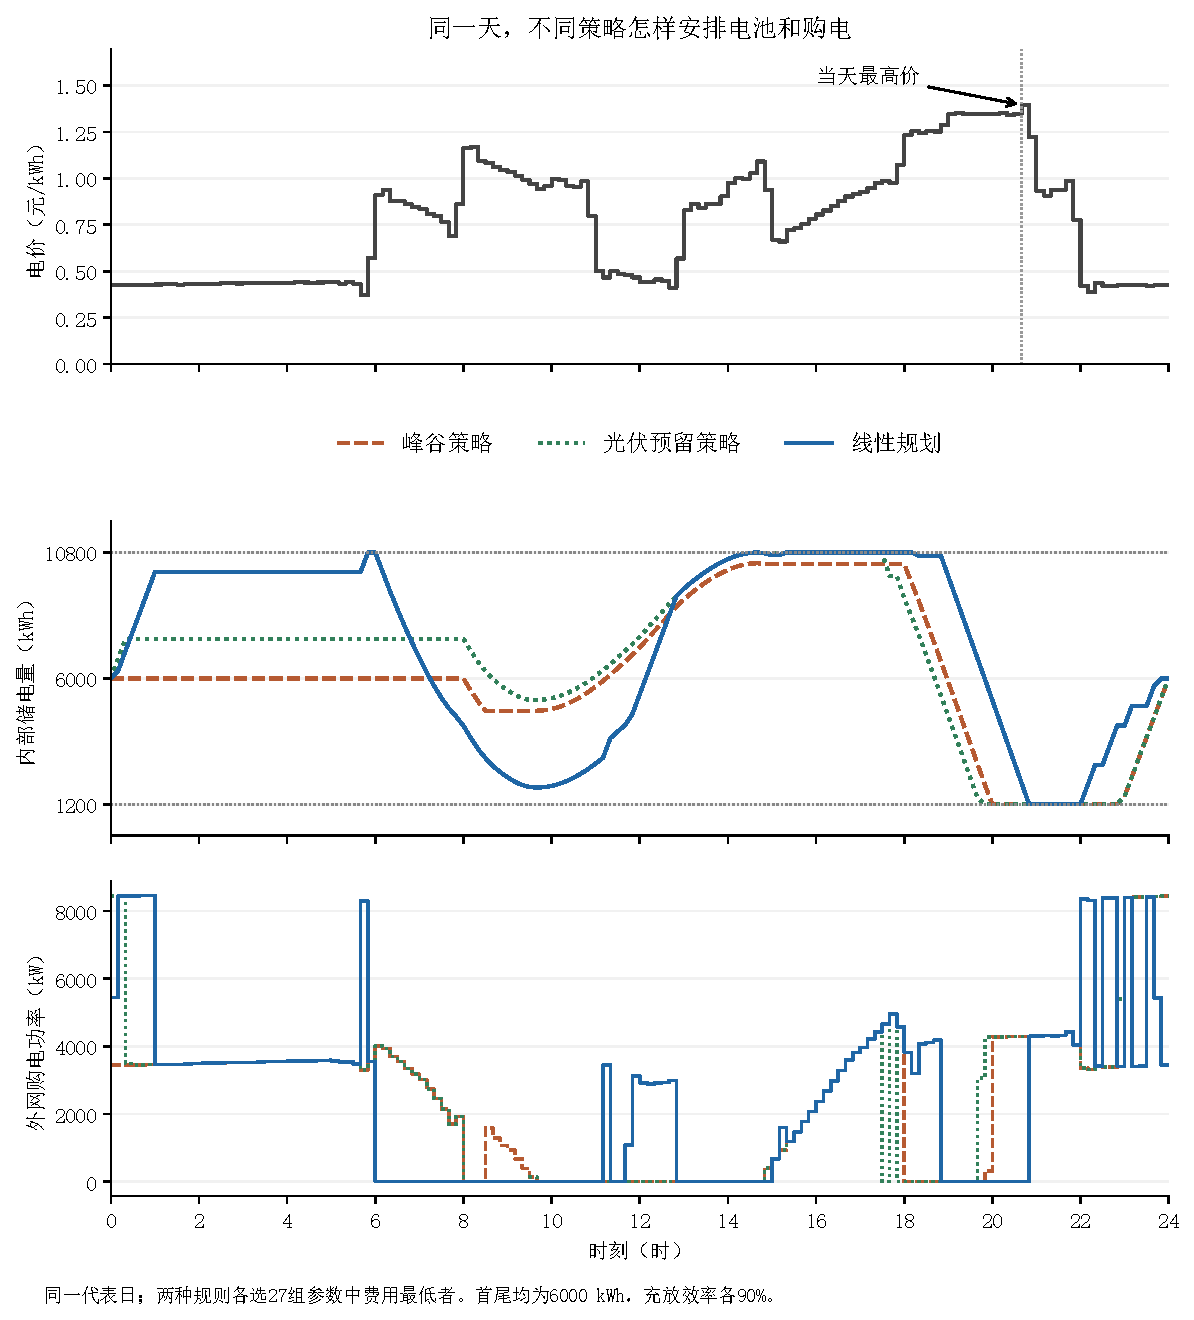
\includegraphics[width=0.95\textwidth]{fig/q1_daily_dispatch.pdf}
    \caption{三种策略在相同代表日下的购电与储能安排}
    \label{fig:q1_2}
\end{figure}

从图~\ref{fig:q1_2}可以看出，线性规划并不是一进入高价时段就立即放空电池，而是会将部分电量保留给后续更高价格的时段。

20:00时，两种规则策略的储电量已经降至 \(1200\,\mathrm{kWh}\) 下限。此时，线性规划仍保留 \(5168.13\,\mathrm{kWh}\)。
当20:40--20:50的电价达到全天最高的 \(1.3952\,\text{元}/\mathrm{kWh}\) 时，线性规划利用储能满足负载，该时段外网购电量为0；另外两种策略则需要购买 \(715.65\,\mathrm{kWh}\) 的高价电。

因此，线性规划节费的关键并不是简单的“低价充、高价放”，而是根据全天价格变化，\textbf{将有限的储能优先留给更有价值的高价时段}。

值得注意的是，线性规划相比峰谷策略多购电 \(1740.28\,\mathrm{kWh}\)。这是因为更多电量经过储能后会产生损耗。但增加的购电主要发生在低价时段，并替代了后续更加昂贵的购电，因此最终总费用仍然更低。

%====================
\subsection{模型检验与敏感性分析}

\subsubsection*{（1）模型结果检验}

为保证求解结果可信，本文重新计算各10分钟时段的供需平衡、储电递推、容量限制、充放电功率和全天费用，并核对日初与日末储电量。

三个初始储电案例中的最大储电递推残差约为
\[
1.34\times10^{-12}\ \mathrm{kWh},
\]
根据求解器的对偶信息独立重算费用下界，该下界与实际可行方案费用的最大差值约为
\[
1.22\times10^{-12}\ \text{元}.
\]

二者均处于数值计算误差范围内，说明所得结果满足模型约束，并支持当前线性规划解的数值最优性。

\subsubsection*{（2）初始储电量敏感性分析}

为考察初始储电量对结果的影响，在其他条件保持不变的情况下，分别取
\[
S_0=1200,\qquad 6000,\qquad 10800\ \mathrm{kWh},
\]
并在每种情况下重新优化，同时要求24:00恢复到相同的初始储电量。

结果如表~\ref{tab:q1_sensitivity}所示。

\begin{table}[H]
    \centering
    \caption{不同初始储电量下的购电费用}
    \label{tab:q1_sensitivity}
    \begin{tabular}{ccc}
        \toprule
        初始储电量/kWh & 全天购电费用/元 & 相比6000 kWh方案 \\
        \midrule
        1200 & 35199.30 & $+0.21\%$ \\
        6000 & \textbf{35126.85} & --- \\
        10800 & 35409.75 & $+0.81\%$ \\
        \bottomrule
    \end{tabular}
\end{table}

三个方案与主方案的费用差异均不足 \(1\%\)，且都会为晚间最高价时段保留电量。这说明初始储电量会改变部分具体购电时刻，但不会改变“将有限储能留给更高价值时段”这一主要调度规律。

需要说明的是，该敏感性分析仅检验了上述三个初始储电量，因此不能据此认定 \(6000\,\mathrm{kWh}\) 是整个允许区间内的最优初始状态。

\section{问题二的模型建立与求解}

\subsection{求解思路}

问题一是在已知代表日供需曲线的情况下安排购电，而问题二要求每天0:00提前制定当天计划，此时当天真实负载和光伏尚未发生。普通电买少了，实际缺口需要按照正常电价的5倍紧急补购；买多了，若无法使用或储存，也仍需支付普通购电费用。因此，本问需要在\textbf{提前购电成本与紧急购电风险之间进行权衡}。

为此，本文依次比较三类方案：首先利用历史同期数据预测负载和光伏；其次引入岭回归和提升树，考察更复杂的预测方法能否降低实际费用；最后在历史预测基础上加入误差准备，针对供需缺口被低估后可能产生的高价紧急购电进行防范。

需要强调的是，本问的最终目标并不是使预测误差最小，而是使普通购电费用与紧急购电费用之和尽可能低。同样大小的预测误差，如果发生在不同电价或不同储电状态下，其经济影响可能完全不同。

因此，本文最终采用“历史分项预测--近期加权准备--跨日线性规划模型”。模型首先分别估计负载和光伏，再根据近期预测误差增加适量准备，随后利用线性规划制定普通购电计划。白天普通订单保持不变，储能设备根据实际供需补充缺口或吸收余电，剩余缺口才通过紧急购电补足。


\subsection{负载与光伏预测}

前文探索性分析表明，负载具有较明显的周重复特征，而光伏更适合参考近期发电水平。因此，本文不直接预测两者的差值，而是分别预测负载和光伏。

设$d$表示日期，$k=1,\ldots,144$表示日内第$k$个10分钟时段，每个时段长度为

\[
\Delta t=\frac{1}{6}\ \mathrm{h}.
\]

负载采用过去4个相同星期位置的同一时段平均，光伏采用最近7天同一时段的平均：

\begin{equation}
\widehat L_{d,k}
=
\frac{1}{4}\sum_{j=1}^{4}L_{d-7j,k},
\qquad
\widehat V_{d,k}
=
\frac{1}{7}\sum_{j=1}^{7}V_{d-j,k}.
\label{eq:q2_forecast}
\end{equation}

即负载主要利用周重复规律，光伏主要利用近期发电水平。历史记录不足时，只对当时已经存在的数据取平均。

为保证每天0:00制定计划时不使用未来信息，式\eqref{eq:q2_forecast}只使用当日零点以前已经发生的数据。虽然附件2保存了全年实际负载和光伏，但当天及之后的真实值均不参与当天预测；本问也不使用问题三才引入的附件3光伏预报。
规划涉及次日时，负载预测匹配次日的星期位置，光伏预测仍使用当前零点之前最近七天的同刻记录。两天的预测共用当前能够获得的历史信息，不因规划延伸到次日而提前使用当天尚未发生的实际值。


\subsection{基于近期误差的准备量}

平均预测能够描述通常的供需水平，但如果连续低估负载或高估光伏，电池可能持续补充缺口并逐渐达到最低储电量。为降低这种风险，本文进一步利用近期预测误差确定购电准备量。

对历史日期$i$，先按该日零点能够获得的信息重建负载和光伏预测，再与随后发生的实际值比较，定义第$k$个时段的净供需预测误差为

\begin{equation}
\varepsilon_{i,k}
=
\left[
(L_{i,k}-V_{i,k})
-
(\widehat L_{i,k}-\widehat V_{i,k})
\right]\Delta t .
\label{eq:q2_error}
\end{equation}

其中，$\varepsilon_{i,k}>0$表示实际供需缺口比预测值更大，即存在低估缺口的风险；负值则表示预测偏保守。

本文将一天划分为六个4小时区间，在最近28天内收集同一时间区间的误差。为使准备量更及时地反映近期变化，对较新的误差赋予更高权重：

\begin{equation}
\omega_{d,i,k}
=
\frac{\beta^{d-1-i}}
{\displaystyle
\sum_{(j,u)\in E_{d,g}}
\beta^{d-1-j}},
\qquad
(i,k)\in E_{d,g},
\label{eq:q2_weight}
\end{equation}

其中，$E_{d,g}$表示最近28天中第$g$个4小时区间的历史误差集合，$\beta$为时间衰减参数。

随后将误差从小到大排列，取加权累计比例达到$\alpha$的位置作为准备依据，并将负值截为0：

\begin{equation}
F_{d,g}(u)
=
\sum_{(i,k)\in E_{d,g}}
\omega_{d,i,k}
\mathbf{1}
\left(
\varepsilon_{i,k}\leq u
\right),
\label{eq:q2_cdf}
\end{equation}

\begin{equation}
b_{d,k}
=
\max
\left\{
0,\,
\inf
\left[
u:F_{d,g(k)}(u)\geq\alpha
\right]
\right\}.
\label{eq:q2_reserve}
\end{equation}

本文取

\[
\alpha=0.7,\qquad \beta=0.7.
\]

其中，$\alpha$控制准备程度，$\beta$控制历史误差随时间的衰减速度，两者含义不同。准备量$b_{d,k}$被加入预测净需求，由后续优化模型统一安排，并不意味着每个时段直接多购买固定数量的电。

预测窗口和准备量参数的选择依据在后文统一说明。每天计算预测值和准备量时，只使用该决策时点以前的数据；但近期加权方法的提出参考了全年误差诊断，因此后续全年比较用于评价本题数据下的费用取舍，不视为完全独立于方法选择的验证。


\subsection{购电与储能优化模型}

\subsubsection*{（1）决策变量与预测净需求}

为减弱单日末端边界对储能决策的影响，每天0:00向前规划48小时，共288个10分钟时段，但只固定当天前144个时段的普通购电计划。

也就是说，模型会考虑午夜以后仍可能存在的用电需求，但不会提前锁定第二天的正式普通购电订单。
根据预测负载、光伏和准备量，定义规划期内第$t$个时段的预测净需求为

\begin{equation}
r_t
=
(\widehat L_t-\widehat V_t)\Delta t+b_t,
\label{eq:q2_net_demand}
\end{equation}

并令

\[
n_t=\max(r_t,0),
\qquad
a_t=\max(-r_t,0),
\]

其中，$n_t$表示预计需要由外网或储能补充的电量，$a_t$表示预计可以用于储能的富余电量。

设置以下连续决策变量：

\[
x_t:\text{外网购电中用于储能充电的电量},
\]

\[
y_t:\text{光伏富余中用于储能充电的电量},
\]

\[
z_t:\text{储能设备向负载输出的电量},
\]

\[
S_t:\text{时段结束时的内部储电量}.
\]

则普通计划购电量为

\begin{equation}
q_t=n_t-z_t+x_t.
\label{eq:q2_purchase}
\end{equation}

其含义是：预计负载缺口先由电池承担一部分，其余由外网补足；同时，模型也可以在合适的时段额外购电给电池充电。


\subsubsection*{（2）目标函数}

48小时规划期内按照固定日内电价计算普通计划费用。为避免模型在规划末端无意义地将储能完全放空，对期末剩余电量赋予参考价值：

\begin{equation}
\min J
=
\sum_{t=1}^{288}p_tq_t
-
\nu S_{288},
\qquad
\nu=0.9p_{00:00}.
\label{eq:q2_objective}
\end{equation}

其中，该期末价值仅用于比较规划方案，并不表示电池可以向外网售电，也不从最终实际购电费用中扣除。


\subsubsection*{（3）约束条件}

为保证购电计划满足储能设备的实际运行要求，设置以下约束。

\textbf{1）储电量递推约束}

储能设备的充电效率和放电效率均为90\%。因此，第$t$个时段结束后的内部储电量为

\begin{equation}
S_t
=
S_{t-1}
+
0.9(x_t+y_t)
-
\frac{z_t}{0.9}.
\label{eq:q2_soc}
\end{equation}

其中，$x_t+y_t$表示进入储能设备的外侧充电量，$z_t$表示储能设备实际向负载输出的电量。充入100 kWh电量时，内部储电量增加90 kWh；向负载输出90 kWh时，内部储电量减少100 kWh。


\textbf{2）储电容量约束}

为避免储能设备过度充电或放电，内部储电量必须保持在允许范围内：

\begin{equation}
1200
\leq
S_t
\leq
10800.
\label{eq:q2_soc_bound}
\end{equation}

该约束保证储能设备始终处于题目规定的安全运行区间。


\textbf{3）充电约束}

外网充电量$x_t$不得为负，光伏充电量$y_t$不能超过该时段预计的光伏富余量$a_t$：

\begin{equation}
x_t\geq0,
\qquad
0\leq y_t\leq a_t.
\label{eq:q2_charge_source}
\end{equation}

储能最大充电功率为5000 kW，每个调度时段为10分钟，因此单个时段的总充电量满足

\begin{equation}
x_t+y_t
\leq
5000\Delta t
=
833.33\ \mathrm{kWh}.
\label{eq:q2_charge_limit}
\end{equation}


\textbf{4）放电约束}

储能放电量不能超过该时段的预计负载缺口$n_t$，同时受到最大放电功率限制：

\begin{equation}
0
\leq
z_t
\leq
\min
\left\{
n_t,\,
5000\Delta t
\right\}.
\label{eq:q2_discharge_limit}
\end{equation}

该约束避免储能向负载提供超过实际需求的电量，也保证放电功率不超过设备上限。


\textbf{5）普通购电非负约束}

各时段的普通计划购电量不能为负：

\begin{equation}
q_t\geq0.
\label{eq:q2_purchase_nonnegative}
\end{equation}


\textbf{6）初始储电状态约束}

每天进行48小时滚动规划时，规划起点的储电量取当天0:00实际剩余的电量：

\begin{equation}
S_0=S_{d,0}.
\label{eq:q2_initial_soc}
\end{equation}

问题二不再要求每天0:00与24:00的储电量相同。当天实际运行结束后的储电量继续作为下一天的初始状态，从而保持储能设备在全年运行过程中的连续性。


\subsection{日内实际供电与跨日运行}

每天0:00完成预测、误差准备和线性规划后，得到当天144个时段的普通购电订单。白天普通订单保持不变，但储能充放电可以根据已经发生的真实负载和光伏进行调整。

运行时首先由光伏直接满足负载。设某时段实际负载电量和光伏电量分别为$l$和$v$，则光伏直供后剩余负载记为$h$。

若实际剩余负载超过普通购电量，则优先由电池在储电量和放电功率允许范围内补充，剩余部分才进行紧急购电：

\begin{equation}
z
=
\min
\left\{
h-q,\,
5000\Delta t,\,
0.9(S-1200)
\right\},
\qquad
e=h-q-z.
\label{eq:q2_emergency}
\end{equation}

其中，$e$为紧急购电量。即使电池仍有存量，若已经接近1200 kWh下限或受到5000 kW放电功率限制，也可能无法完全补足当前缺口。

若普通购电已经能够覆盖实际剩余负载，则优先将实际光伏富余和普通购电余量用于储能充电，并受到储能容量和充电功率限制。

因此，第$d$天实际购电费用为

\begin{equation}
C_d
=
\sum_{k=1}^{144}
\left(
p_kq_{d,k}
+
5p_ke_{d,k}
\right),
\label{eq:q2_daily_cost}
\end{equation}

并满足跨日状态传递

\begin{equation}
S_{d+1,0}=S_{d,144}.
\label{eq:q2_cross_day}
\end{equation}

由此形成从零点制定计划、日内储能吸收偏差、必要时紧急补购，到日末库存传递至下一天的连续调度过程。

全年运行从2025年1月1日0:00的6000 kWh开始。首日没有更早历史，普通购电订单采用问题一的购电安排。按区间起点映射后，附件2缺少1月1日00:00--00:10的实际记录，仅该区间借用附件1的午夜供需值启动，且不将这一参考值纳入预测训练。

1月2日起，负载按已有的同星期记录、光伏按最近三天同刻记录形成启动预测；历史不足时回退到可用的同刻记录，完全没有记录时才采用附件1参考。1月份的实际运行轨迹保持不变，后续选出的预测窗口不倒填到此前决策。由这条连续轨迹得到2月1日0:00的内部储电量为8592.69 kWh，各候选均从这一共同状态开始比较，此后分别承接自身前一日的实际剩余电量。


\subsection{参数依据与方案比较}

模型选择时，以最终实际购电费用作为主要评价标准。预测误差较小通常有利，但同样大小的误差若出现在高价时段，或连续消耗储能库存，仍可能造成较高紧急购电费用。

因此，本文比较了历史分项预测、岭回归、提升树以及加入误差准备后的多种方案。各方案使用相同的电价、储能设备、起始状态、规划长度和实际供电规则。

预测窗口先利用1月份数据比较负载1周或4周、光伏3天或7天的组合，选取负载4周、光伏7天。分位参数$\alpha=0.7$在1月份三档正准备量设置中费用最低，但当月不加准备量的费用更低，说明提前增加准备是否划算仍取决于实际供需变化。随后根据全年误差诊断引入近期权重，并利用1月8--31日的历史回放，在0.7、0.8和0.9三档衰减参数中选取$\beta=0.7$。

$\beta$决定旧误差保留多少影响。取0.7时，最近一天、再前一天和再前两天的相对权重依次为1、0.7和0.49，权重约每1.94天减半；按权重集中程度折算，信息量约相当于5.67个等权日期。因而，虽然窗口覆盖28天，准备量主要跟随近期约一周的误差变化。

若$\beta$更大，旧误差保留更久，准备量对近期变化的反应较慢；若继续减小，例如取0.6，等效日期数约降至4天，准备量更容易受少数异常日影响。本文未对小于0.7的取值完成全年费用比较，因此将0.7作为适应速度与历史信息量之间的折中，而不声称它是连续参数范围内的最优值。这里的权重仅反映记录的新旧程度，不是将预测值乘以0.7，也不是给负载和光伏分配重要性。

其中，岭回归和提升树主要以提高预测精度为目标，并未直接考虑预测误差在不同电价与储能状态下造成的经济损失。因此，预测误差较小并不一定意味着最终购电费用更低。相比之下，近期加权准备直接针对缺口低估可能引起的高价紧急购电风险。

2月1日至12月31日334天的实际费用比较如表\ref{tab:q2_model_compare}所示。

\begin{table}[htbp]
\centering
\caption{不同方案的334天实际购电费用}
\label{tab:q2_model_compare}
\begin{tabular}{lccc}
\hline
方案 & 普通电费/万元 & 紧急电费/万元 & 总电费/万元 \\
\hline
历史分别预测，无误差准备
& 1218.58 & 374.70 & 1593.28 \\
分别岭回归，无误差准备
& 1210.27 & 446.88 & 1657.15 \\
分别提升树，无误差准备
& 1218.25 & 343.71 & 1561.96 \\
历史分别预测，等权误差准备
& 1295.99 & 107.05 & 1403.04 \\
历史分别预测，近期加权准备
& \textbf{1297.96} & \textbf{60.43} & \textbf{1358.38} \\
\hline
\end{tabular}
\end{table}

近期加权准备方案的普通电费比等权准备方案增加约1.97万元，但紧急电费减少约46.63万元，因此总费用减少约44.66万元，降幅为3.18\%。与不设置误差准备的历史预测方案相比，总费用下降约14.74\%。

提升树虽然降低了部分预测误差，却没有取得最低的实际购电费用。这进一步说明，本问应围绕最终经济成本选择方案，而不能仅以预测精度决定模型优劣。

因此，候选方案的实际费用比较支持了本文采用“历史分项预测--近期加权准备--跨日线性规划”的结构，但该比较仅针对已实际测试的模型与参数组合，不表示已经排除了所有其他预测方法。


\subsection{全年结果与指定日期分析}

2025年2月1日至12月31日共334天，最终方案总费用为

\[
\boxed{13583810.84\ \text{元}},
\]

其中普通购电费用为

\[
12979560.57\ \text{元},
\]

紧急购电费用为

\[
604250.27\ \text{元}.
\]

完整10分钟结果保存于\texttt{result2.xlsx}。


\subsubsection*{（1）月度费用分析}

图\ref{fig:q2_monthly_cost}给出了各月普通购电费、紧急购电费，以及近期加权方案相对于等权准备方案的节省金额。

\begin{figure}[htbp]
    \centering
    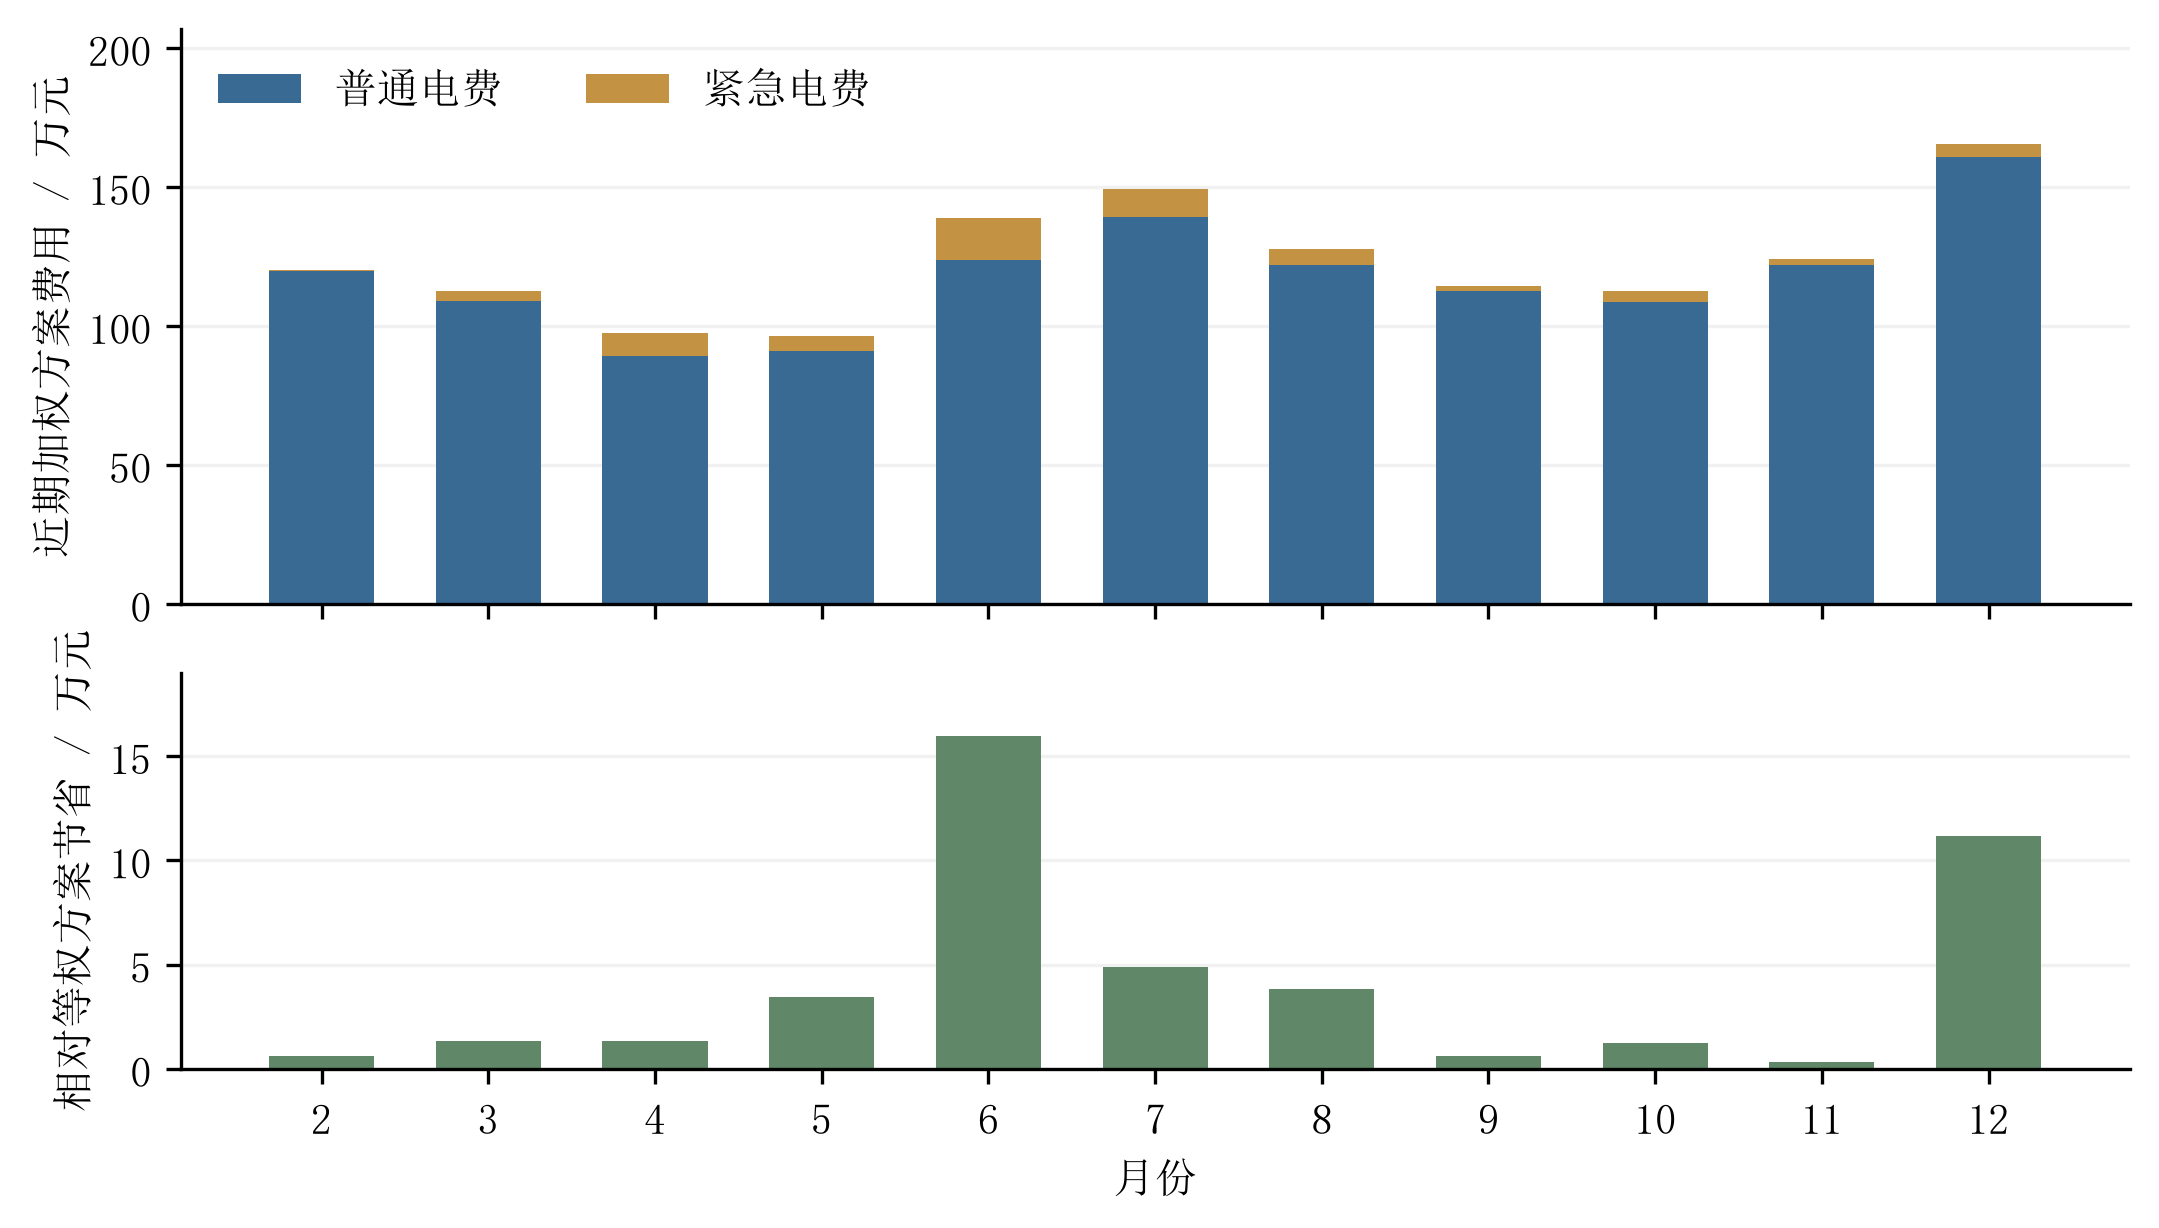
\includegraphics[width=0.95\textwidth]{fig/monthly_cost.png}
    \caption{近期加权准备方案的月度费用及相对等权准备的节省}
    \label{fig:q2_monthly_cost}
\end{figure}

由图\ref{fig:q2_monthly_cost}可见，各月份费用主要由普通购电组成，但紧急购电由于价格较高，对总费用仍有明显影响。11个月合计均取得节省，其中6月和12月的贡献较大。

这说明近期误差能够为购电准备提供有效信息，但其效果会随着具体供需条件变化。逐日结果并不保证每一天都比等权方案更便宜，因此其优势应从全年总费用角度评价。


\subsubsection*{（2）指定日期购电结果}

题目指定四个日期的购电和费用结果如表\ref{tab:q2_specified_purchase}所示。

\begin{table}[H]
\centering
\caption{指定日期的计划购电及全天费用}
\label{tab:q2_specified_purchase}
\begin{tabular}{lrrrr}
\hline
项目 & 3月20日 & 6月21日 & 9月23日 & 12月21日 \\
\hline
10:00--10:10
& 0.00 & 0.00 & 0.00 & 0.00 \\
12:00--12:10
& 610.16 & 0.00 & 484.48 & 943.63 \\
14:00--14:10
& 0.00 & 0.00 & 0.00 & 0.00 \\
16:00--16:10
& 434.90 & 116.65 & 453.86 & 798.03 \\
18:00--18:10
& 716.29 & 437.88 & 826.38 & 742.86 \\
20:00--20:10
& 0.00 & 0.00 & 5.90 & 0.00 \\
全天计划购电量/kWh
& 64232.05 & 40298.69 & 68385.07 & 95446.27 \\
全天紧急购电量/kWh
& 329.52 & 0.00 & 6.38 & 0.00 \\
全天购电合计/kWh
& 64561.57 & 40298.69 & 68391.44 & 95446.27 \\
普通电费/元
& 39469.74 & 22323.80 & 42730.05 & 61249.77 \\
紧急电费/元
& 2298.74 & 0.00 & 43.00 & 0.00 \\
总电费/元
& 41768.47 & 22323.80 & 42773.04 & 61249.77 \\
\hline
\end{tabular}
\end{table}

各日全天结果均由完整144个10分钟区间汇总得到，不能由表中展示的六个指定时段直接相加得到。


\subsubsection*{（3）指定日期储能运行结果}

各指定日期的实际充放电情况如表\ref{tab:q2_storage}所示。

\begin{table}[H]
\centering
\caption{指定日期的实际充放电量及日首尾储电量}
\label{tab:q2_storage}
\begin{tabular}{llrrrr}
\hline
时间段 & 项目 & 3月20日 & 6月21日 & 9月23日 & 12月21日 \\
\hline
00:00--04:00 & 充电
& 1504.96 & 309.75 & 1739.22 & 1830.47 \\
& 放电
& 185.93 & 229.12 & 2.78 & 227.55 \\

04:00--08:00 & 充电
& 1138.95 & 286.60 & 53.65 & 1476.38 \\
& 放电
& 4670.35 & 1949.50 & 5934.88 & 729.24 \\

08:00--12:00 & 充电
& 5327.26 & 10134.27 & 4409.06 & 4706.14 \\
& 放电
& 3265.56 & 0.00 & 2387.94 & 8254.51 \\

12:00--16:00 & 充电
& 4465.10 & 21.43 & 6147.58 & 8347.54 \\
& 放电
& 369.53 & 0.00 & 521.04 & 2318.98 \\

16:00--20:00 & 充电
& 169.64 & 115.05 & 221.91 & 19.45 \\
& 放电
& 5340.10 & 5107.80 & 4920.36 & 4873.96 \\

20:00--24:00 & 充电
& 4438.27 & 8636.77 & 8446.30 & 8360.50 \\
& 放电
& 3424.22 & 3022.72 & 3633.41 & 3626.10 \\
\hline
0:00储电量/kWh & 
& 8919.73 & 3543.84 & 9214.11 & 8886.94 \\
24:00储电量/kWh &
& 5086.49 & 9642.73 & 8796.25 & 8897.44 \\
\hline
\end{tabular}
\end{table}

表中的充、放电量按储能设备外侧计量，日初和日末储电量按内部电量计量。一个4小时区间内同时存在充电量和放电量，仅表示不同10分钟时段执行了不同动作，并非同一时段同时充放电。


\subsubsection*{（4）指定日期紧急购电}

按照赛题要求的表格形式，将四个指定日期的紧急购电结果整理如表\ref{tab:q2_emergency_purchase}所示。

\begin{table}[H]
\centering
\caption{问题二指定日期的紧急购电量（kWh）}
\label{tab:q2_emergency_purchase}
\small
\setlength{\tabcolsep}{4pt}
\begin{tabular}{|c|c|c|c|c|c|c|c|}
\hline
\multicolumn{2}{|c|}{2025.3.20} & \multicolumn{2}{c|}{2025.6.21} & \multicolumn{2}{c|}{2025.9.23} & \multicolumn{2}{c|}{2025.12.21} \\
\hline
时间段 & 购电量 & 时间段 & 购电量 & 时间段 & 购电量 & 时间段 & 购电量 \\
\hline
20:40--20:50 & 329.52 & 无紧急购电 & 0.00 & 20:30--20:40 & 6.38 & 无紧急购电 & 0.00 \\
\hline
\end{tabular}
\end{table}

四个指定日期中，3月20日和9月23日发生紧急购电，6月21日和12月21日均未发生紧急补购。


\subsubsection*{（5）储能对预测偏差的缓冲作用}

为进一步解释紧急购电产生的原因，图\ref{fig:q2_specified_days}选取3月20日和6月21日进行比较。

\begin{figure}[H]
    \centering
    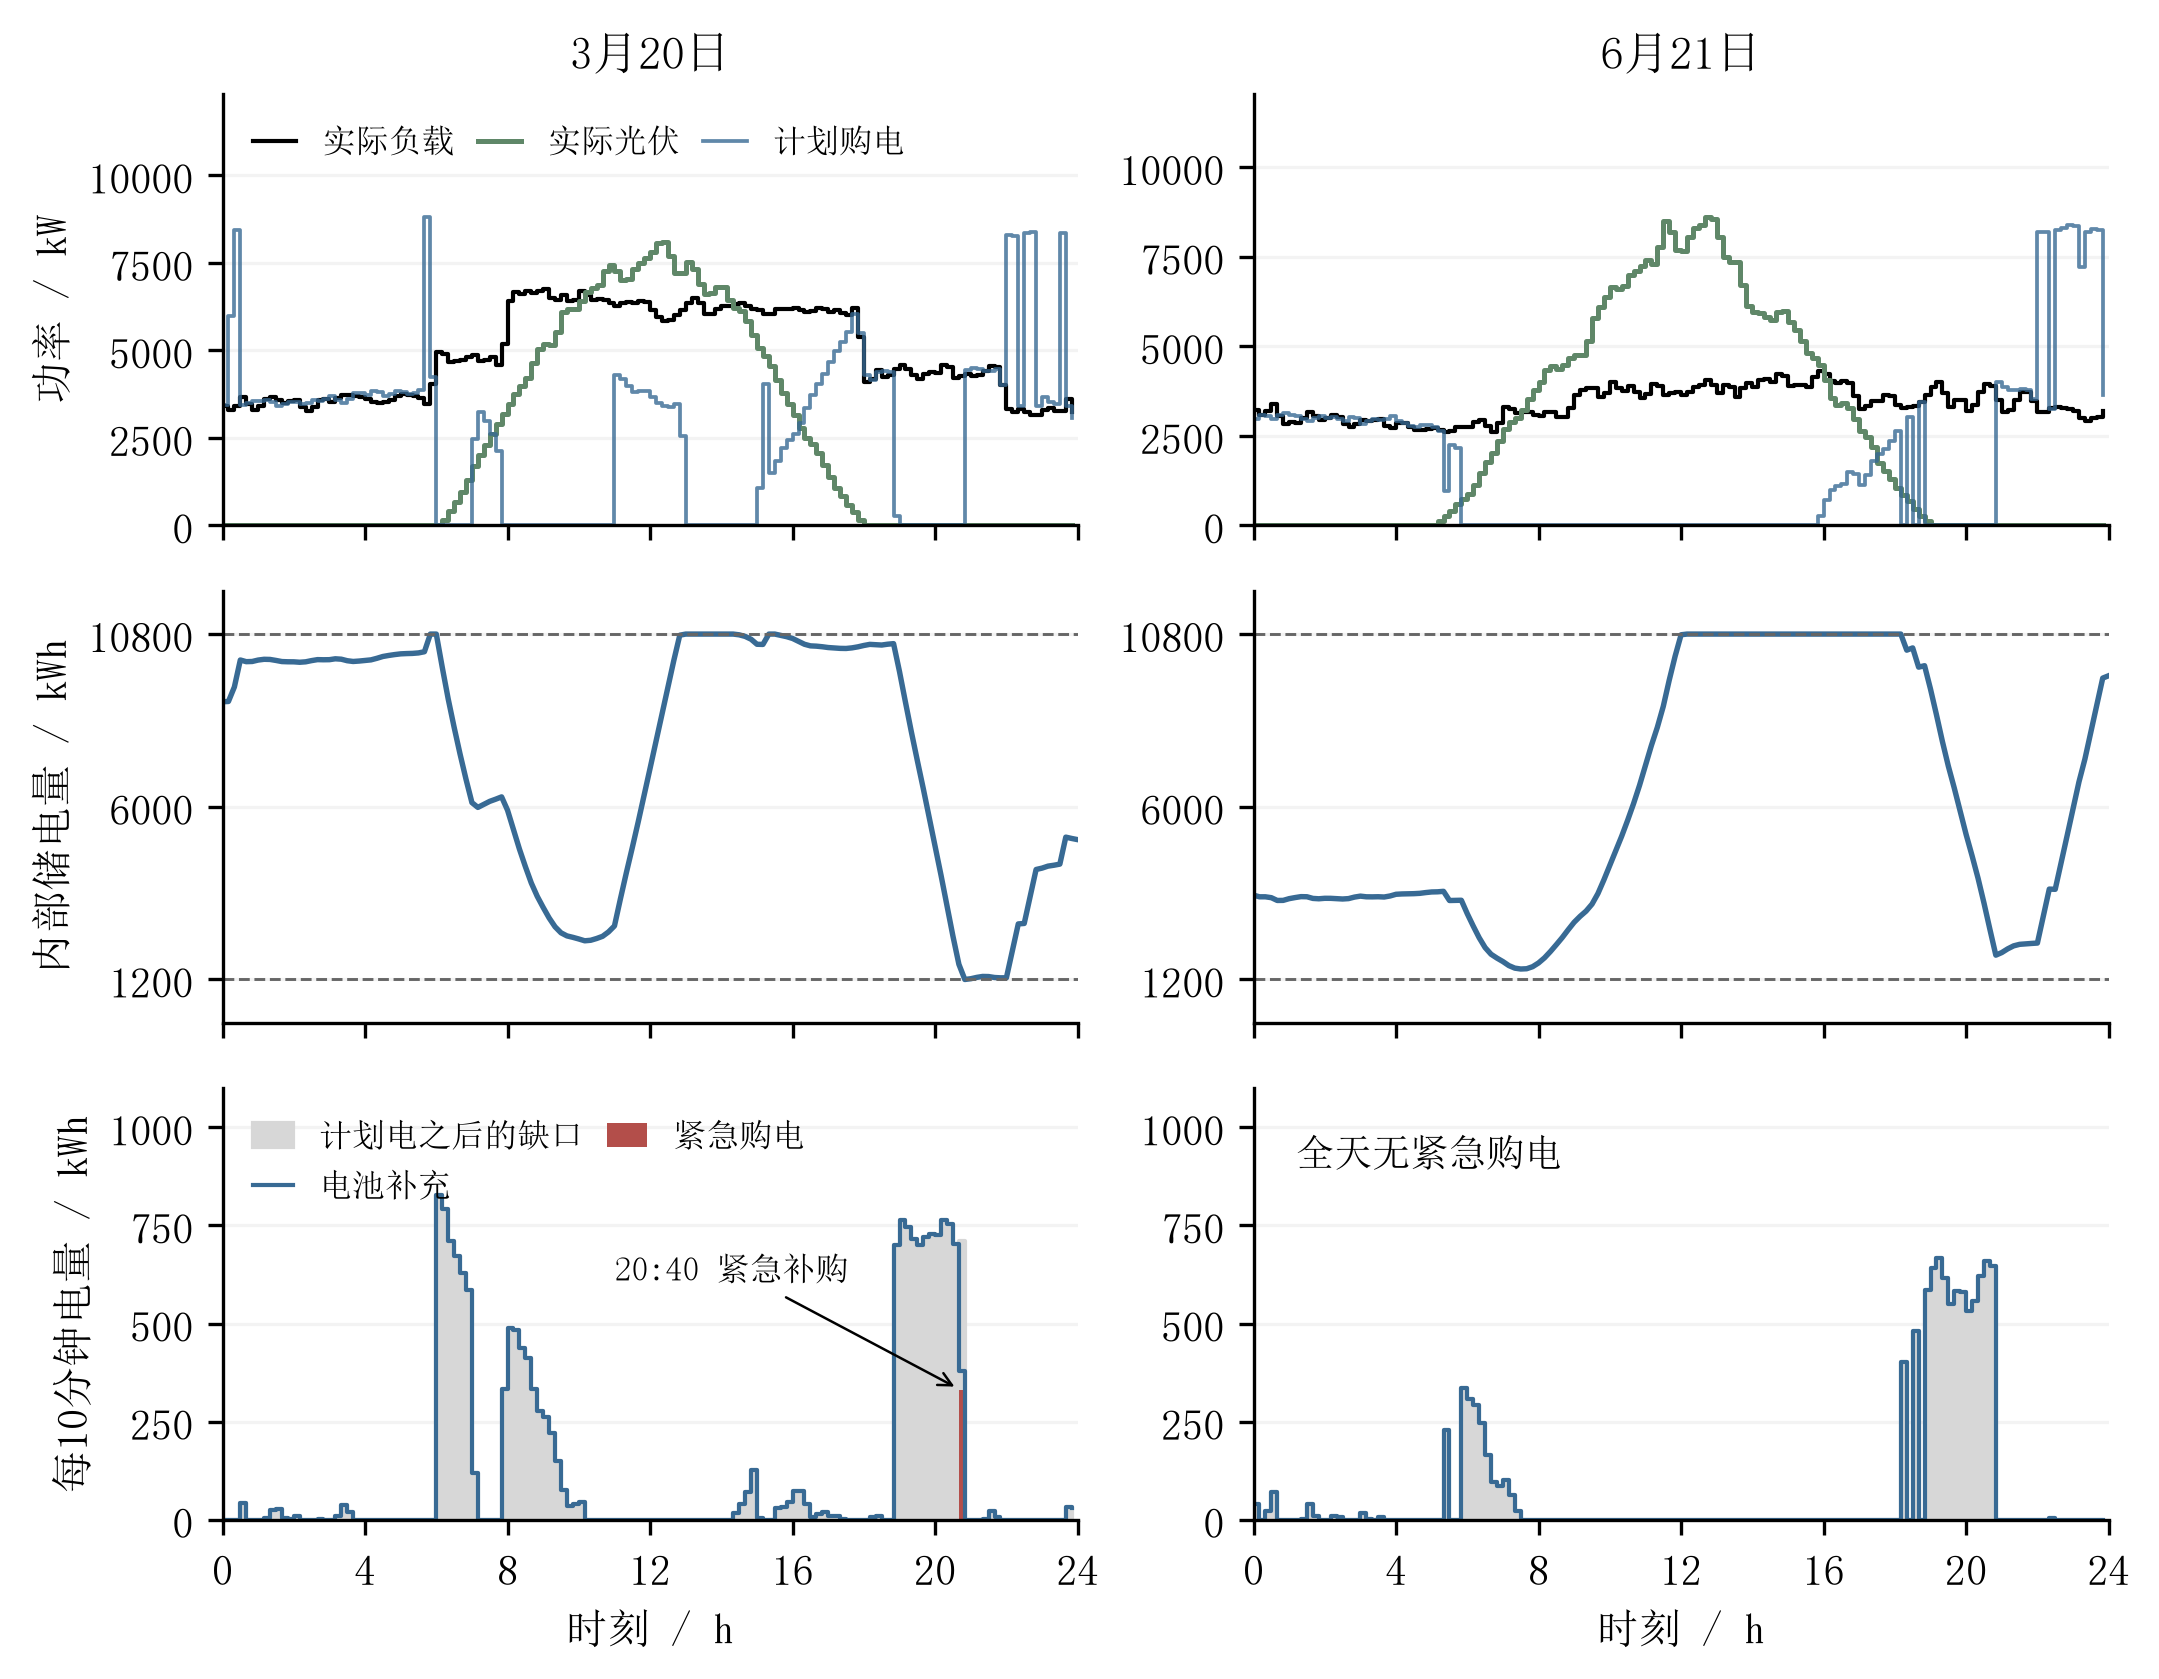
\includegraphics[width=\textwidth]{fig/specified_days.png}
    \caption{两个指定日期的供需、储电量与缺口补充情况}
    \label{fig:q2_specified_days}
\end{figure}

3月20日的大部分供需缺口都能够由储能设备补充，但20:40开始时内部储电量仅剩1622.06 kWh。继续放电后达到1200 kWh下限，因此仍有329.52 kWh的缺口只能通过紧急购电补足。

相比之下，6月21日白天实际光伏较多，储能能够吸收光伏并在后续时段释放，因此全天没有发生紧急购电。

由图\ref{fig:q2_specified_days}可以看出，判断是否需要紧急购电，不能只比较全天总供需量，而应同时考虑\textbf{缺口发生的时刻、当时剩余储电量以及储能的最大放电能力}。


\subsection{灵敏度检验与风险分析}

为考察准备量参数对最终费用的影响，分别改变分位参数$\alpha$和时间衰减参数$\beta$，其余条件保持不变，并以

\[
\alpha=\beta=0.7
\]

作为基准。

图\ref{fig:q2_sensitivity}给出了不同参数下普通电费、紧急电费和总费用的变化。

\begin{figure}[H]
    \centering
    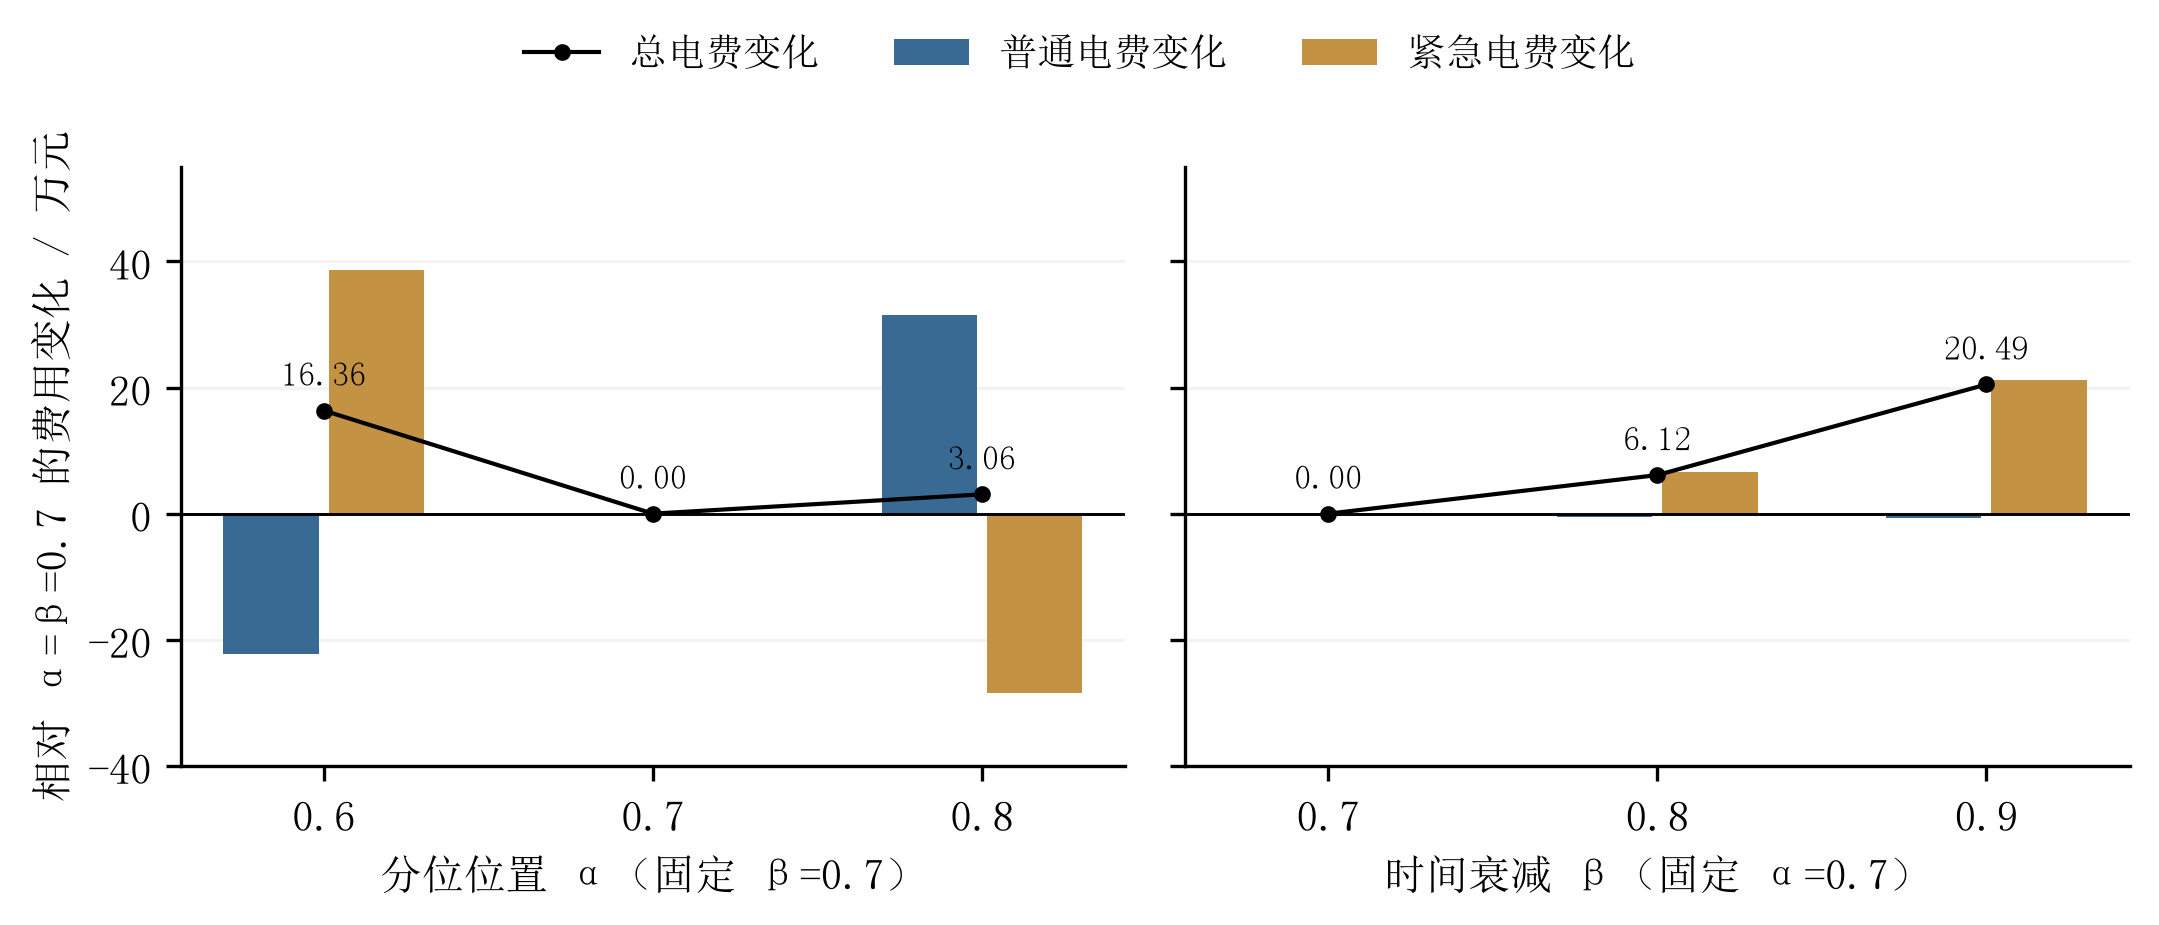
\includegraphics[width=0.95\textwidth]{fig/sensitivity.png}
    \caption{准备程度与近期权重对购电费用的影响}
    \label{fig:q2_sensitivity}
\end{figure}

当固定$\beta=0.7$时，将$\alpha$提高到0.8后，紧急购电天数由156天减少至102天，但普通购电费用的增加超过紧急购电费用的下降，使总费用反而增加约3.06万元；当$\alpha$降至0.6时，准备不足使总费用增加约16.36万元。

当固定$\alpha=0.7$时，将$\beta$提高到0.8和0.9，总费用分别增加约6.12万元和20.49万元。较大的$\beta$使旧误差保留更高权重，从而降低准备量对近期供需变化的响应速度。

因此，\textbf{准备程度并不是越高越好}。准备不足会增加昂贵的紧急购电，而准备过多又会提高普通购电成本。在本文实际检验的参数范围内，$\alpha=\beta=0.7$的综合费用较低，但不能据此认为其是所有连续参数取值中的唯一最优解。
规划长度的选择还需兼顾跨日供电风险。将规划窗口缩短为24小时后，总费用减少3215.61元，降幅约为0.024\%，但发生紧急购电的天数增加，最长连续紧急补购时间由200分钟延长至340分钟，期末库存也有所减少。因此，本文在费用接近的情况下保留48小时规划，以兼顾跨日库存与连续缺电风险。去掉期末库存参考价值后，本次实际总费用未变，故不将该项单独作为已证实的节费来源。

进一步逐段检查表明，最终方案仍有部分日期发生紧急购电。这并不意味着模型失效，而是说明储能设备只能在其容量和功率范围内缓冲预测误差；当电池已经达到最低库存或受到放电功率限制时，紧急购电仍不可避免。

为考察连续预测偏差的影响，利用此前已经发生的三天误差片段，分别构造持续低估负载、高估光伏及二者同时发生的情景。在三类所测情景下，近期加权方案的总费用仍比等权方案低3.09\%--3.52\%，说明其费用优势在这些连续偏差下得以保留。不过，近期权重也可能跟随短暂异常而增加订单，不能保证每天都更便宜。上述结果来自同一年数据和有限情景，尚不能证明相同参数在其他年份或其他微网中仍然有效。

\section{问题三的模型建立与求解}

\subsection{日内新信息下的求解思路}

问题三在问题二的基础上增加了新的信息和新的代价：每天0:00先制定购电计划，
6:00、12:00和18:00还能获得新的光伏预报，并允许修改尚未执行的订单，
但修改订单本身需要付费。因此，本问的关键不只是提高预测精度，
而是判断新的信息是否值得转化为新的购电订单。

新预报并不意味着必须修改订单。若预测变化较小，电池可以自行吸收偏差，
则修改订单反而可能增加费用；若预计缺口较大、储能又不足，
提前调整订单则可能比事后按5倍电价紧急购电更加经济。

针对这一特点，本文设置四种候选方案：
\begin{enumerate}
    \item 直接采用官方光伏预报；
    \item 利用历史误差融合官方预报；
    \item 采用提升树修正官方预报；
    \item 在融合预报基础上加入近期误差准备。
\end{enumerate}

四种方案均采用相同的日内滚动调度方式，并以全年实际购电费用作为最终评价依据。
综合预报信息的可解释性和紧急购电风险，本文重点研究并最终采用
\[
\boxed{\text{历史融合预报--动态安全准备--日内滚动规划模型}}
\]
作为问题三的购电策略。


\subsection{光伏预报修正与动态安全准备}

\subsubsection*{（1）融合官方预报与近期历史}

负载继续沿用问题二的方法，根据过去四个相同星期位置的历史负载进行预测。
光伏则优先利用附件3提供的官方预报。由于官方预报按整点给出，而购电计划以10分钟为一个时段，
因此先对同一发布时间下相邻两个整点的光伏预报进行线性插值，
将小时级信息转换为10分钟功率序列。

设当前发布时间为$r$，附件3在该时点发布的官方光伏预报为$F_{r,t}$。对目标时刻$t$，取发布时点以前最近七个可用同刻实际光伏值的均值作为历史参考$H_{r,t}$，则融合后的光伏预测为
\begin{equation}
\widehat{V}_{r,t}
=
w_{r,g}F_{r,t}
+
(1-w_{r,g})H_{r,t}.
\end{equation}

将未来24小时按照提前1--6、7--12、13--18和19--24小时分组。对每个发布时间和提前量组，选取过去28天内、截至当前已经能够核验的预报与实测配对记录，以融合预测的历史平方误差最小为目标确定权重：
\begin{equation}
w_{r,g}
=
\operatorname{clip}_{[0,1]}
\left(
\frac{
\sum (F-H)(V-H)
}{
\sum (F-H)^2
}
\right).
\end{equation}
式中的求和均在对应组的历史配对样本内进行，$V$表示已经发生的实际光伏；$\operatorname{clip}_{[0,1]}$将计算结果限制在0与1之间，使融合结果保持为官方预报与历史参考的加权组合。

当官方预报近期更加准确时，其权重自动增加；当近期历史曲线更可靠时，
历史信息所占比例提高。因此，$w_{r,g}$ 会随发布时间和预测提前量变化，
而不是人为设置一个固定权重。


\subsubsection*{（2）根据近期净需求误差增加安全准备}

即使平均预测更加准确，也仍可能在个别关键时段低估供需缺口。
若少估 $1\,\mathrm{kWh}$ 的缺口，运行时可能需要按5倍电价紧急补购；
但若准备过多，又可能出现普通购电无法使用或储存的情况。

因此，本文直接考察历史上“实际比预测多缺多少电”。定义净需求预测误差为
\begin{equation}
\varepsilon_{i,k}
=
\left[
(L_{i,k}-V_{i,k})
-
(\widehat{L}_{i,k}-\widehat{V}_{i,k})
\right]\Delta t.
\end{equation}

当 $\varepsilon_{i,k}>0$ 时，说明原预测低估了实际供需缺口。

每次重新决策时，只使用此前28天已经发生的误差，
并将一天划分为8个3小时时段。距离当前 $a_j$ 天的历史记录赋予衰减权重
\begin{equation}
\omega_j
\propto
0.7^{a_j}.
\end{equation}

即最近一天权重最高，再早一天乘以0.7，再早两天乘以 $0.7^2$。
随后在每个3小时组内取历史误差的加权0.60分位，并将负值截为0：
\begin{equation}
m_{r,k}
=
\max
\left\{
0,\,
Q_{0.60}^{(\omega)}(\varepsilon)
\right\}.
\end{equation}

这里的0.60表示历史误差排序中的位置，并不表示多购买60\%的电。
该准备量的作用是在普通购电成本和5倍紧急购电风险之间取得平衡。


\subsection{日内滚动购电与储能调度模型}

\subsubsection*{（1）预测供需与决策变量}

综合负载预测、融合光伏预测和安全准备量，定义预计净需求为
\begin{equation}
r_t
=
(\widehat{L}_t-\widehat{V}_t)\Delta t+m_t.
\end{equation}

进一步记
\begin{equation}
n_t=\max(r_t,0),
\qquad
a_t=\max(-r_t,0),
\end{equation}
其中，$n_t$ 表示预计仍需由外网或储能补充的电量，
$a_t$ 表示预计可用于储能的光伏富余量。

每个10分钟时段设置以下主要决策变量：
\begin{itemize}
    \item $q_t$：普通购电订单；
    \item $x_t$：外网购电中用于储能充电的电量；
    \item $y_t$：富余光伏中用于储能充电的电量；
    \item $z_t$：储能设备向负载输出的电量；
    \item $e_t$：预计紧急购电量；
    \item $u_t$：已经订购但预计无法接收的普通电量；
    \item $S_t$：时段结束后的电池内部储电量。
\end{itemize}


\subsubsection*{（2）供需平衡与储能约束}

光伏优先直接满足负载，剩余部分满足
\begin{equation}
q_t-x_t+z_t+e_t-u_t=n_t.
\end{equation}

其中，普通购电既可以直接供给负载，也可以通过 $x_t$ 给储能设备充电；
若普通订单过多且电池无法继续接收，则由 $u_t$ 记录未接收部分。

充、放电效率均为90\%，因此储电状态满足
\begin{equation}
S_t
=
S_{t-1}
+
0.9(x_t+y_t)
-
\frac{z_t}{0.9}.
\end{equation}

同时满足储电容量约束
\begin{equation}
1200\leq S_t\leq10800.
\end{equation}

储能设备最大充电和放电功率均为5000~kW，
因此每个10分钟时段最多充入或放出
\[
5000\times\frac{1}{6}
=
833.33\ \mathrm{kWh}.
\]

各类电量均须非负，光伏充电量不能超过预计富余，同时满足充、放电功率限制：
\begin{equation}
\begin{aligned}
&x_t,y_t,z_t,e_t,u_t,q_t\geq0,\qquad y_t\leq a_t,\\
&x_t+y_t\leq5000\Delta t,\qquad z_t\leq5000\Delta t,\\
&z_t+e_t\leq n_t.
\end{aligned}
\end{equation}
其中，最后一项限制储能与紧急购电共同补充的电量不超过负载缺口；放电功率上限则单独限制电池在一个时段内能够输出的电量。

每天的初始储电量直接取上一天24:00的实际剩余电量，
不再要求每日0:00和24:00的储电量相等。


\subsubsection*{（3）订单调整费用}

设每天0:00确定的原始订单为 $q_t^0$，
执行前最后一次调整得到的订单为 $q_t^F$。

按本文采用的结算方式，增加订单的部分按原电价的1.5倍收费；减少订单时，扣除取消部分的原购电款，同时支付该部分原电价50\%的调整费。因此，最终普通购电及调整费用可统一表示为
\begin{equation}
C_{\mathrm{ord}}
=
\sum_t
\left[
p_tq_t^F
+
\frac{1}{2}p_t
\left|
q_t^F-q_t^0
\right|
\right].
\end{equation}

同一个时段即使经过多次调整，也只比较最终订单与零点订单之间的净变化，
不重复累计中间修改产生的费用。
上述普通结算已经包含最终订单电费和调整费，不再另加零点原订单的费用。若以$e_{d,k}^{\mathrm{act}}$表示实际运行中的紧急购电量，则统计期内总费用为
\begin{equation}
C=\sum_{d,k}\left[
p_kq_{d,k}^{F}
+\frac{1}{2}p_k\left|q_{d,k}^{F}-q_{d,k}^{0}\right|
+5p_ke_{d,k}^{\mathrm{act}}
\right].
\end{equation}
规划中的$e_t$用于估计未来补购代价，实际结算则采用运行后得到的$e_{d,k}^{\mathrm{act}}$，二者不混用。


\subsubsection*{（4）目标函数}

每次重新决策时，从当前时刻规划至次日24:00。记$T_r$为该规划期内的全部时段，$D_r$为当天尚未执行、已有零点订单的时段。普通购电和预计紧急购电费用在整个规划期内计算，调整费仅针对$D_r$中的订单：
\begin{equation}
\min J=
\sum_{t\in T_r}p_t(q_t+5e_t)
+\frac{1}{2}\sum_{t\in D_r}p_t\delta_t
-\nu S_T,
\end{equation}
其中
\begin{equation}
\delta_t\geq q_t-q_t^0,\qquad
\delta_t\geq q_t^0-q_t,\qquad t\in D_r.
\end{equation}
零点首次制定订单时尚无调整，调整费项取零；次日部分只用于安排跨日库存，不作为已经下单的订单收取调整费。

期末价值系数沿用问题二的$\nu=0.9p_{00:00}$。末端库存项$-\nu S_T$为规划期后的用电保留参考价值，仅参与方案选择，不作为收入从实际购电费用中扣除。

上述目标函数及约束均为线性关系，因此采用线性规划进行求解。


\subsection{日内滚动求解过程}

每天按照0:00、6:00、12:00和18:00四个决策时刻滚动运行：

\begin{enumerate}
    \item \textbf{0:00：}
    读取已有历史、当前真实储电量和0:00官方预报，
    形成负载预测、融合光伏预测及安全准备量，制定当天零点原计划；

    \item \textbf{6:00：}
    读取新的官方预报和当前真实储电量，
    重新计算未来预测和准备量，只修改6:00以后尚未执行的订单；

    \item \textbf{12:00和18:00：}
    按照相同方式继续更新，
    已经执行的订单保持不变；

    \item \textbf{实际运行：}
    光伏优先满足负载，普通订单不足时先由电池补充，
    储能仍无法满足的部分才进行紧急购电；

    \item \textbf{跨日衔接：}
    24:00按照最终订单相对零点订单的净变化完成结算，
    并将真实日末储电量传递给下一天。
\end{enumerate}

本问从问题二共同启动过程得到的2月1日0:00内部储电量8592.69 kWh开始运行。2025年2月1日至12月31日共334天，每天求解4次，共完成1336次滚动线性规划。每次求解均以当前实际库存为初值，次日规划只辅助安排跨日库存，不提前锁定次日订单。


\subsection{候选方案比较与最终模型选择}

为保证比较公平，各候选方案采用相同的负载预测、设备参数、
初始库存、实际供电方式和费用结算规则，仅改变光伏预测方式及风险准备方法。
完整334天的费用比较如表~\ref{tab:q3_candidate}所示。

\begin{table}[H]
\centering
\caption{问题三候选方案的334天费用比较}
\label{tab:q3_candidate}
\small
\setlength{\tabcolsep}{4pt}
\begin{tabular}{lcccc}
\hline
方案
& 普通结算/万元
& 紧急购电/万元
& 总费用/万元
& 紧急购电天数 \\
\hline
直接采用官方预报
& 1289.96 & 127.56 & 1417.51 & 280 \\

历史误差融合预报
& 1276.36 & 132.51 & 1408.87 & 282 \\

提升树修正预报
& 1279.46 & 136.80 & 1416.26 & 285 \\

\textbf{融合预报并增加近期误差准备}
& \textbf{1294.35}
& \textbf{20.31}
& \textbf{1314.65}
& \textbf{164} \\
\hline
\end{tabular}
\end{table}

直接利用历史信息融合官方预报后，总费用由1417.51万元下降至1408.87万元，
说明官方预报和近期历史记录能够相互补充。

但历史融合方案的紧急购电费用仍达到132.51万元，
说明平均预测更加准确，仍可能在少数关键时段低估实际缺口。

加入动态安全准备后，普通结算增加约17.98万元，
但紧急购电费用减少约112.20万元，
总费用降低94.22万元。
因此，最终采用
\[
\boxed{\text{历史融合预报--动态安全准备--日内滚动规划模型}}.
\]

该方案的优势并不来自模型更加复杂，
而是同时利用当天官方预报、近期历史误差，
并针对5倍紧急购电风险保留适量安全余量。


\subsection{全年结果与指定日期分析}

\subsubsection*{（1）全年费用结果}

最终方案在334天内的普通结算费用为
\[
12943484.52\ \text{元},
\]
紧急购电费用为
\[
203050.97\ \text{元},
\]
因此总费用为
\[
\boxed{13146535.49\ \text{元}}.
\]

全年紧急购电量为
\[
35685.12\ \mathrm{kWh},
\]
共有164天至少出现一次紧急购电。

如图~\ref{fig:q3_monthly}所示，
2月至12月各月相对于初始融合方案均实现费用下降，
主要收益来自减少高价紧急购电。

但是，月度节省并不代表每天都更便宜。
逐日比较中共有250天费用下降、59天增加、25天基本不变。
同时，全年仍存在443358.10~kWh未接收普通订单，
说明动态安全准备本身也需要付出一定代价。

\begin{figure}[H]
    \centering
    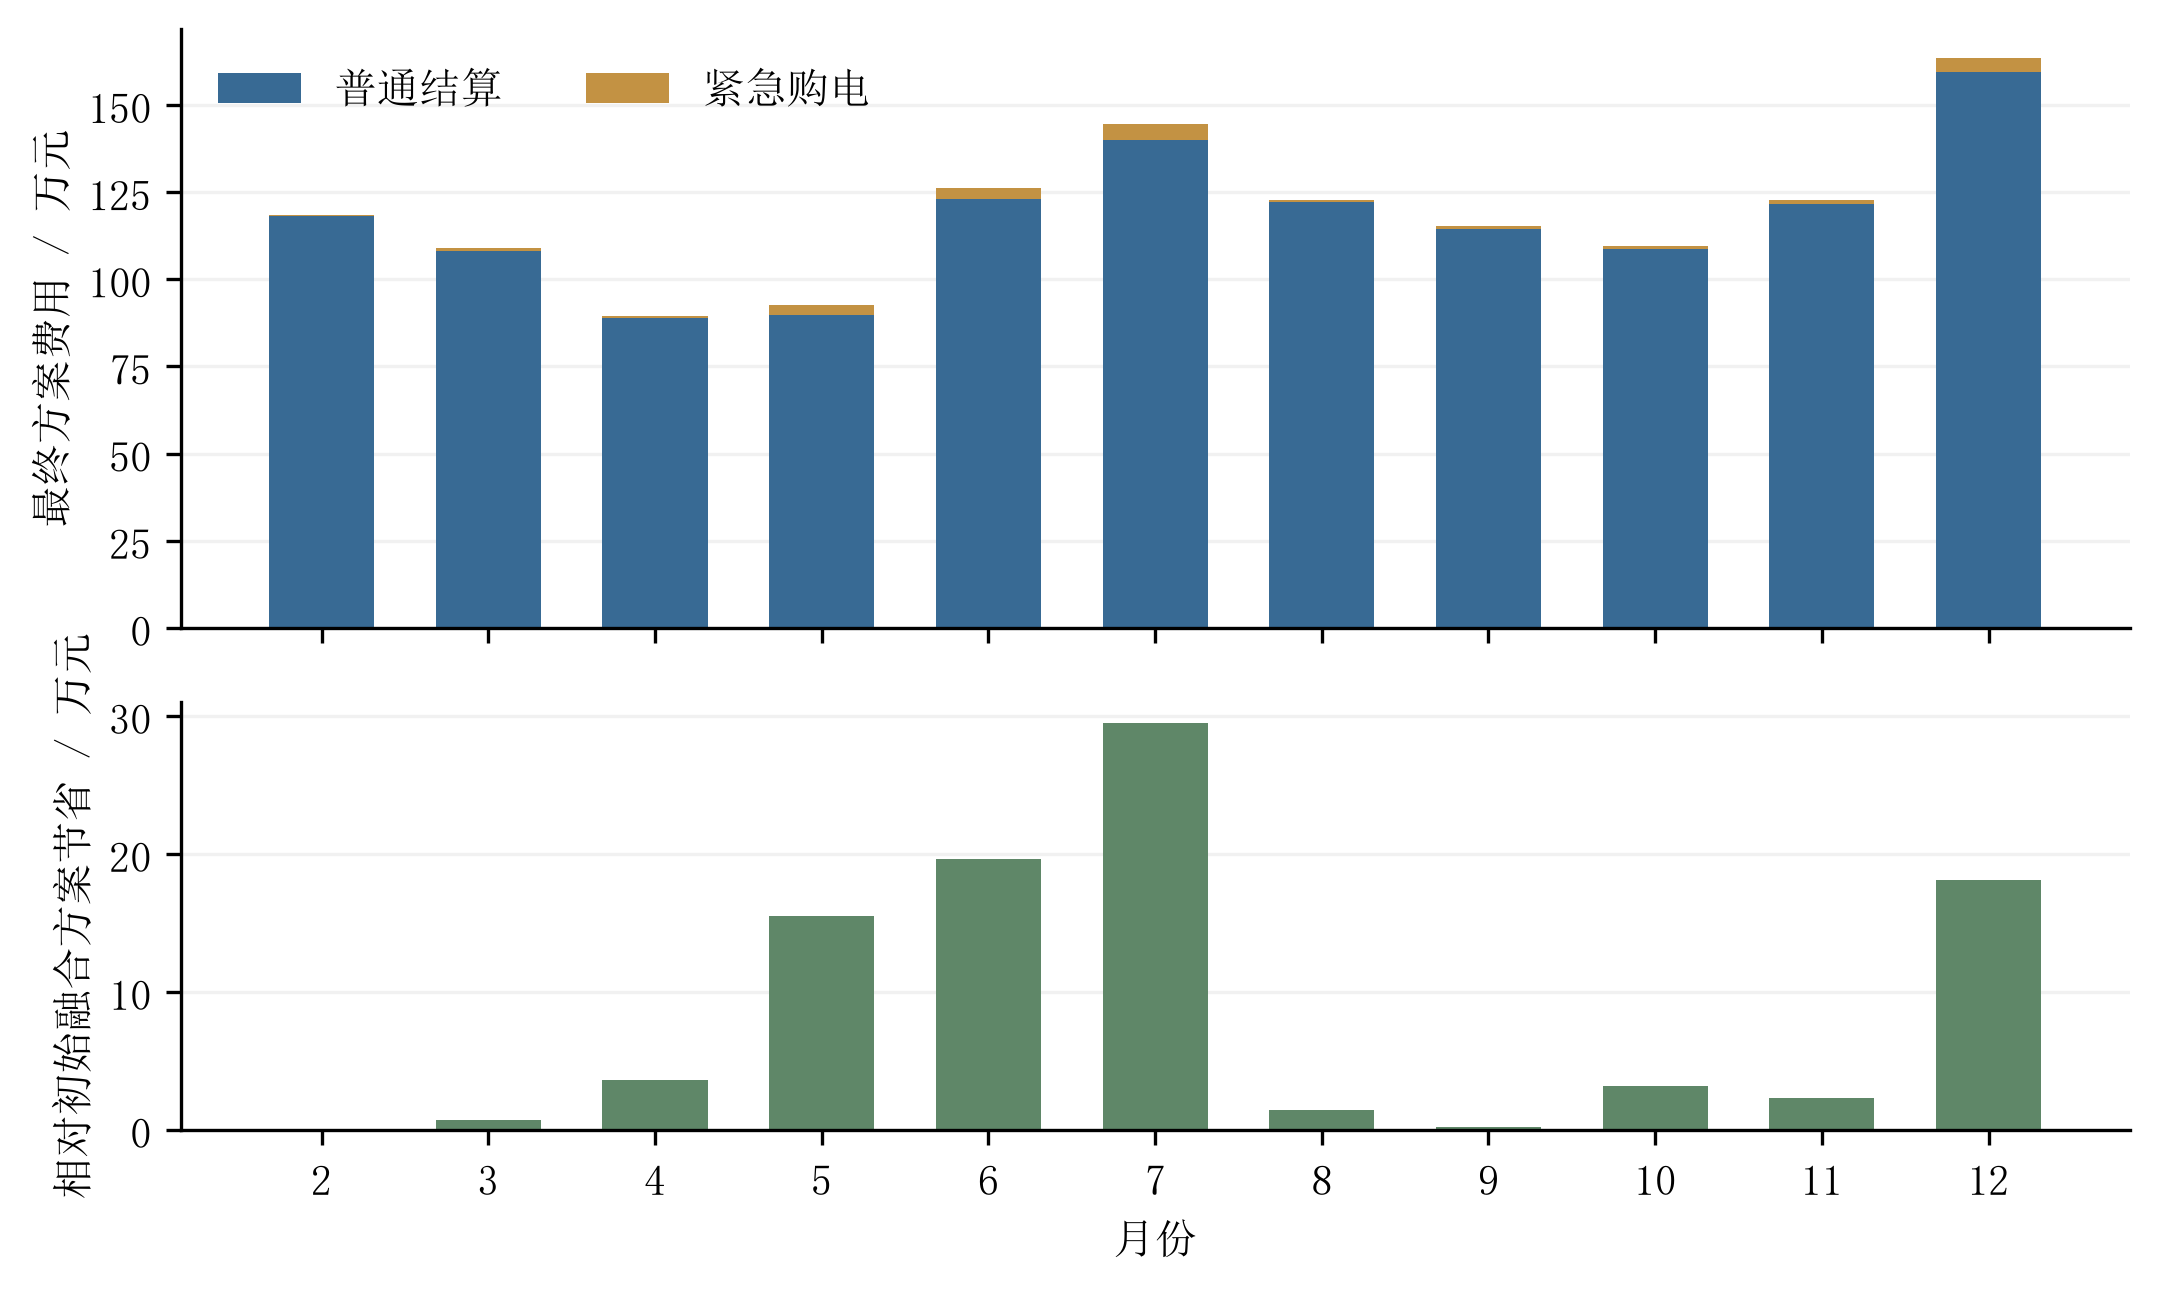
\includegraphics[width=0.90\textwidth]{fig/final_monthly.png}
    \caption{最终方案的月度费用及相对初始融合方案的节省}
    \label{fig:q3_monthly}
\end{figure}


\subsubsection*{（2）指定日期零点原计划}

题目指定日期在0:00制定的部分原始购电计划如表~\ref{tab:q3_original_order}所示。

\begin{table}[htbp]
\centering
\caption{指定日期零点原计划的部分时段购电量}
\label{tab:q3_original_order}
\begin{tabular}{ccccc}
\hline
时间段
& 3月20日
& 6月21日
& 9月23日
& 12月21日 \\
\hline
10:00--10:10 & 0.00   & 0.00   & 0.00   & 0.00 \\
12:00--12:10 & 586.14 & 0.00   & 436.19 & 948.82 \\
14:00--14:10 & 0.00   & 0.00   & 0.00   & 0.00 \\
16:00--16:10 & 489.39 & 110.71 & 472.88 & 806.52 \\
18:00--18:10 & 716.29 & 432.73 & 827.44 & 731.68 \\
20:00--20:10 & 0.00   & 0.00   & 5.90   & 0.00 \\
\hline
\end{tabular}
\end{table}


\subsubsection*{（3）日内调整后的购电结果}

经过6:00、12:00和18:00的滚动调整后，
指定日期的最终普通订单和全天费用如表~\ref{tab:q3_final_order}所示。

\begin{table}[htbp]
\centering
\caption{指定日期调整后订单及全天费用}
\label{tab:q3_final_order}
\begin{tabular}{lcccc}
\hline
项目
& 3月20日
& 6月21日
& 9月23日
& 12月21日 \\
\hline
10:00--10:10 & 0.00 & 0.00 & 0.00 & 0.00 \\
12:00--12:10 & 586.14 & 0.00 & 436.19 & 975.93 \\
14:00--14:10 & 0.00 & 0.00 & 0.00 & 0.00 \\
16:00--16:10 & 471.19 & 68.81 & 475.08 & 834.21 \\
18:00--18:10 & 716.29 & 424.29 & 809.29 & 731.64 \\
20:00--20:10 & 0.00 & 0.00 & 5.90 & 0.00 \\
\hline
全天原计划购电量/kWh
& 64012.35 & 39766.06 & 68933.65 & 94785.86 \\

全天最终普通订单/kWh
& 62868.01 & 39547.19 & 69071.70 & 95867.85 \\

全天紧急购电量/kWh
& 95.59 & 14.64 & 6.38 & 45.47 \\

普通结算费用/元
& 39587.60 & 21816.59 & 43609.00 & 62120.52 \\

紧急购电费用/元
& 666.80 & 58.34 & 43.00 & 198.32 \\

\textbf{全天总费用/元}
& \textbf{40254.40}
& \textbf{21874.93}
& \textbf{43652.00}
& \textbf{62318.84} \\
\hline
\end{tabular}
\end{table}

可以看出，日内调整并不是统一增加或减少购电量。
例如3月20日最终订单低于零点原计划，
而12月21日最终订单高于原计划，
说明模型会根据新的光伏信息和当前储电状态重新判断未来供需。


\subsubsection*{（4）指定日期储能运行}

四个指定日期的实际充放电及日首、日末储电量如表~\ref{tab:q3_storage}所示。

\begin{table}[htbp]
\centering
\caption{指定日期的实际充放电及日首尾储电量}
\label{tab:q3_storage}
\begin{tabular}{llcccc}
\hline
时间段 & 项目
& 3月20日
& 6月21日
& 9月23日
& 12月21日 \\
\hline
00:00--04:00 & 充电 & 1556.01 & 240.54  & 1739.21 & 2064.56 \\
              & 放电 & 185.93  & 348.67  & 2.78    & 215.12 \\

04:00--08:00 & 充电 & 951.71  & 257.49  & 57.67   & 1564.44 \\
              & 放电 & 5205.35 & 1744.95 & 6257.36 & 777.76 \\

08:00--12:00 & 充电 & 4142.68 & 10134.27 & 4754.81 & 4462.12 \\
              & 放电 & 3265.56 & 0.00     & 2387.94 & 8634.27 \\

12:00--16:00 & 充电 & 6169.03 & 344.79  & 6385.35 & 8760.52 \\
              & 放电 & 289.59  & 0.00    & 403.62  & 2070.34 \\

16:00--20:00 & 充电 & 138.06  & 83.56   & 94.38   & 7.92 \\
              & 放电 & 4894.55 & 5209.77 & 4784.01 & 5009.17 \\

20:00--24:00 & 充电 & 4405.05 & 8583.09 & 8446.30 & 8322.00 \\
              & 放电 & 3677.85 & 3028.38 & 3633.41 & 3628.73 \\
\hline
0:00  & 内部储电量 & 8873.79 & 3246.87 & 9214.11 & 8630.73 \\
24:00 & 内部储电量 & 5034.71 & 9446.49 & 9133.92 & 8699.27 \\
\hline
\end{tabular}
\end{table}

表中某个4小时区间同时存在充电量和放电量，
表示该区间内部不同的10分钟时段采取了不同动作，
并不表示储能设备在同一个10分钟时段同时充电和放电。


\subsubsection*{（5）紧急购电与典型日期分析}

指定日期的紧急购电结果如表~\ref{tab:q3_emergency}所示。

\begin{table}[H]
\centering
\caption{问题三指定日期的紧急购电量（kWh）}
\label{tab:q3_emergency}
\small
\setlength{\tabcolsep}{4pt}
\begin{tabular}{|c|c|c|c|c|c|c|c|}
\hline
\multicolumn{2}{|c|}{2025.3.20} & \multicolumn{2}{c|}{2025.6.21} & \multicolumn{2}{c|}{2025.9.23} & \multicolumn{2}{c|}{2025.12.21} \\
\hline
时间段 & 购电量 & 时间段 & 购电量 & 时间段 & 购电量 & 时间段 & 购电量 \\
\hline
20:40--20:50 & 95.59 & 07:20--07:30 & 14.64 & 20:30--20:40 & 6.38 & 08:00--08:10 & 9.20 \\
\hline
-- & -- & -- & -- & -- & -- & 10:50--11:00 & 36.26 \\
\hline
\end{tabular}
\end{table}
表中各时段电量分别保留两位小数，全天合计由未舍入的逐段结果计算，因此显示值相加可能与全天合计存在0.01 kWh的差异。

图~\ref{fig:q3_days}进一步展示了3月20日和9月23日的实际负载、
实际光伏、零点订单、最终订单、储电状态以及缺口补充过程。

3月20日20:40附近，电池已经接近1200~kWh的储电下限，
仍有95.59~kWh缺口无法继续由储能补足，因此需要紧急购电。
9月23日仅在20:30--20:40发生6.38~kWh紧急购电。

这说明是否需要紧急购电不能只比较全天总电量，
还必须考虑缺口出现的具体时刻、当时剩余储电量以及储能设备的放电能力。

\begin{figure}[H]
    \centering
    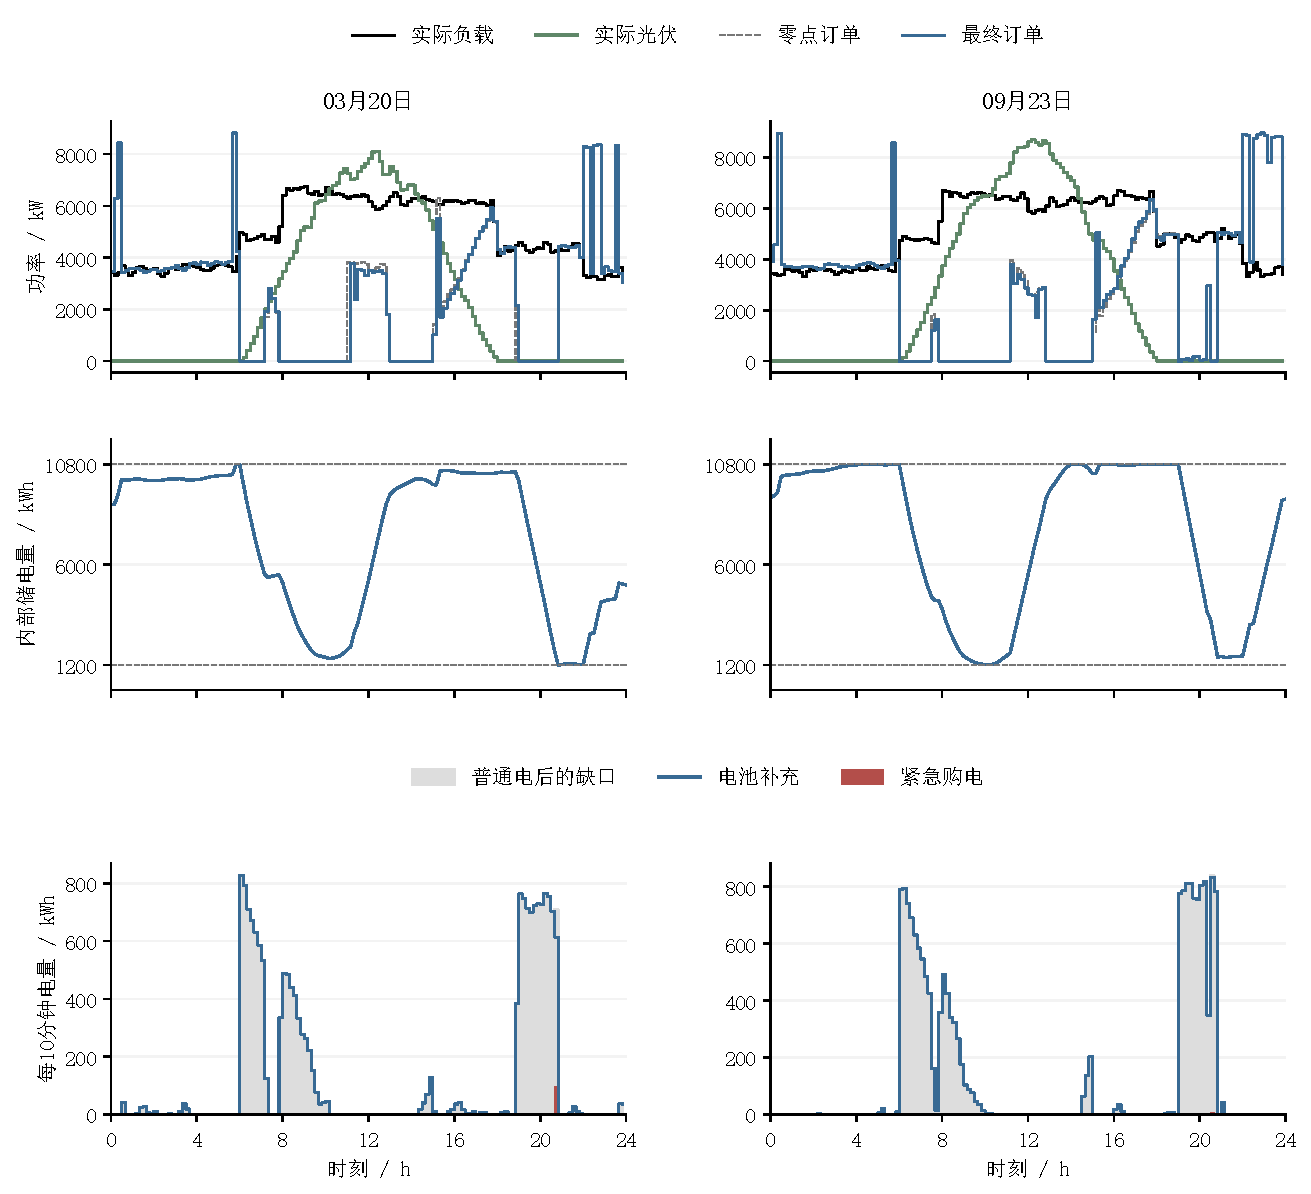
\includegraphics[width=0.95\textwidth]{fig/q3_specified_days.pdf}
    \caption{两个指定日期的供需、库存和缺口补充过程}
    \label{fig:q3_days}
\end{figure}


\subsection{日内新预报的实际费用价值}

题目要求判断是否有必要使用6:00、12:00和18:00的新光伏预报。

若直接比较零点固定订单与完整问题三方案，
会同时混入日内实际供需反馈、真实储电量更新和新官方预报三种作用。
因此，在直接使用官方预报的同一策略下设置三个逐步增加信息的对照方案，
结果如表~\ref{tab:q3_info}和图~\ref{fig:q3_info}所示。

\begin{table}[H]
\centering
\caption{日内反馈与新增官方预报的费用比较}
\label{tab:q3_info}
\begin{tabular}{lc}
\hline
方案 & 总费用/万元 \\
\hline
零点订电，全天不修改订单
& 1614.80 \\

允许日内反馈和改单，但不使用后发官方预报
& 1439.29 \\

允许日内反馈和改单，并使用新官方预报
& 1417.51 \\
\hline
\end{tabular}
\end{table}

开放日内实际反馈和订单调整后，
总费用首先减少175.51万元；
在相同的反馈和改单权限下，
进一步使用6:00、12:00和18:00的新官方预报，
又减少21.78万元。

因此，对于题目提出的“是否需要引入其他时刻预报”，本文认为
\[
\boxed{\text{需要引入日内新预报}}.
\]

在相同反馈和调整条件下，
使用新官方预报将费用由1439.29万元降低至1417.51万元，
额外节省21.78万元，约为1.51\%。

但这并不表示三个发布时间具有完全相同的价值，
也不表示每次收到新预报后都必须修改订单。
是否改单仍需结合预测变化、调整费用和当前储电状态共同决定。

\begin{figure}[H]
    \centering
    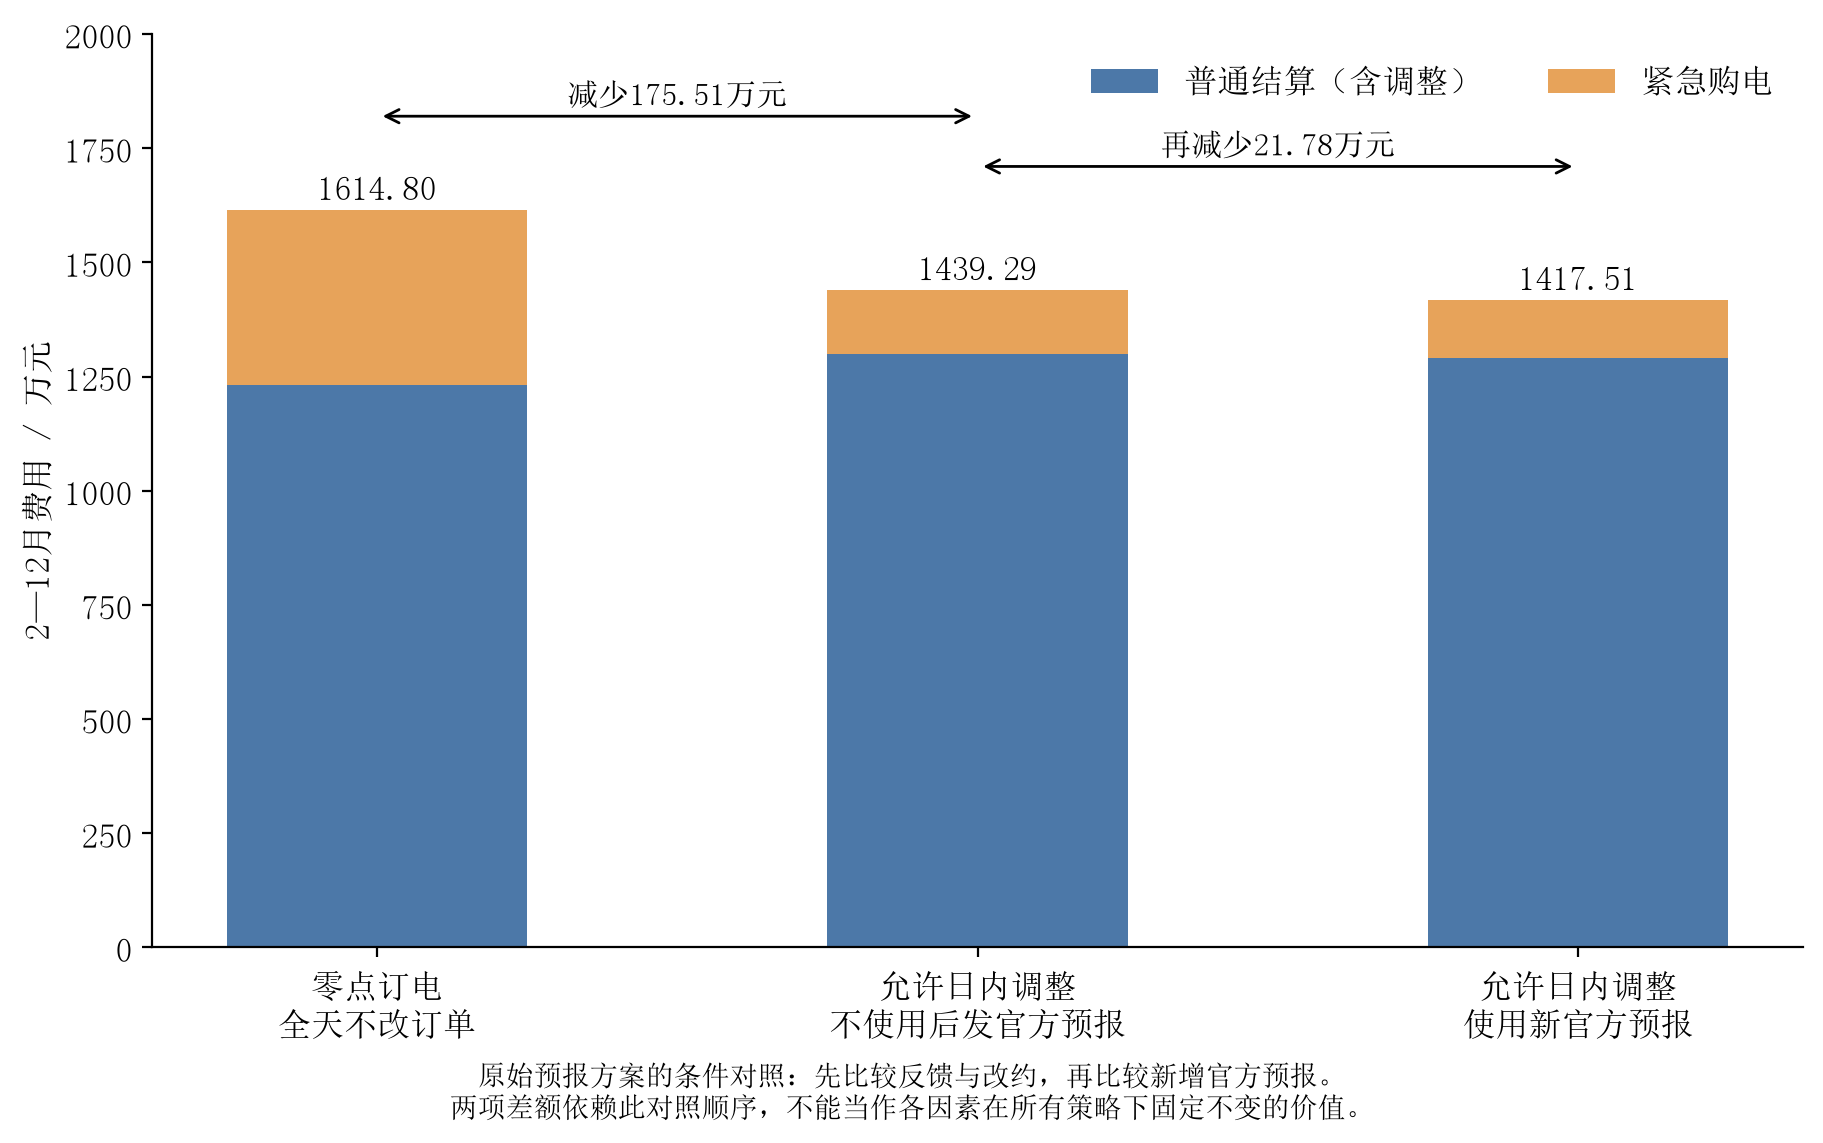
\includegraphics[width=0.85\textwidth]{fig/information_value.png}
    \caption{日内反馈、改单与新增官方预报的费用价值}
    \label{fig:q3_info}
\end{figure}


\subsection{参数灵敏度与模型可信度}

动态安全准备量依赖误差分位、日期衰减、误差分组宽度和历史窗口。
为了避免参数选择过于主观，
本文在其他条件保持不变的情况下分别进行灵敏度比较，
结果如图~\ref{fig:q3_parameter}所示。

\subsubsection*{（1）误差分位}

在0.55--0.80的分位范围内，
0.60对应的全年总费用最低。
继续提高分位虽然能够减少紧急购电，
但普通购电和未接收订单随之增加，
最终总费用反而上升。

\subsubsection*{（2）日期衰减}

时间衰减参数分别取0.7、0.8和1.0时，
总费用约为
\[
1314.65,\qquad
1318.88,\qquad
1342.54
\quad \text{万元}.
\]

因此，近期误差应在当前购电决策中发挥更大的作用，
最终取衰减参数为0.7。

\subsubsection*{（3）误差分组宽度}

比较1、2、3、4和6小时的误差分组后，
3小时方案总费用最低。
同时，3小时恰好将每个6小时预报更新区间划分为前后两段，
能够兼顾日内误差差异与历史样本稳定性。

\subsubsection*{（4）历史窗口}

历史窗口分别取14、28和56天时，
相对于28天方案的费用差仅为十余元。
因此，模型对这一参数并不敏感，
最终采用能够覆盖4个完整星期的28天历史窗口。

此外，逐次撤去安全准备量以及强制保留零点订单一定比例的方案均会增加总费用。
因此，最终模型在0:00、6:00、12:00和18:00四次决策中均重新计算并保留安全准备，
同时不额外限制向下调整订单的比例，
而由模型根据新预报、调整费用和真实库存自行决定是否改单。

\begin{figure}[H]
    \centering
    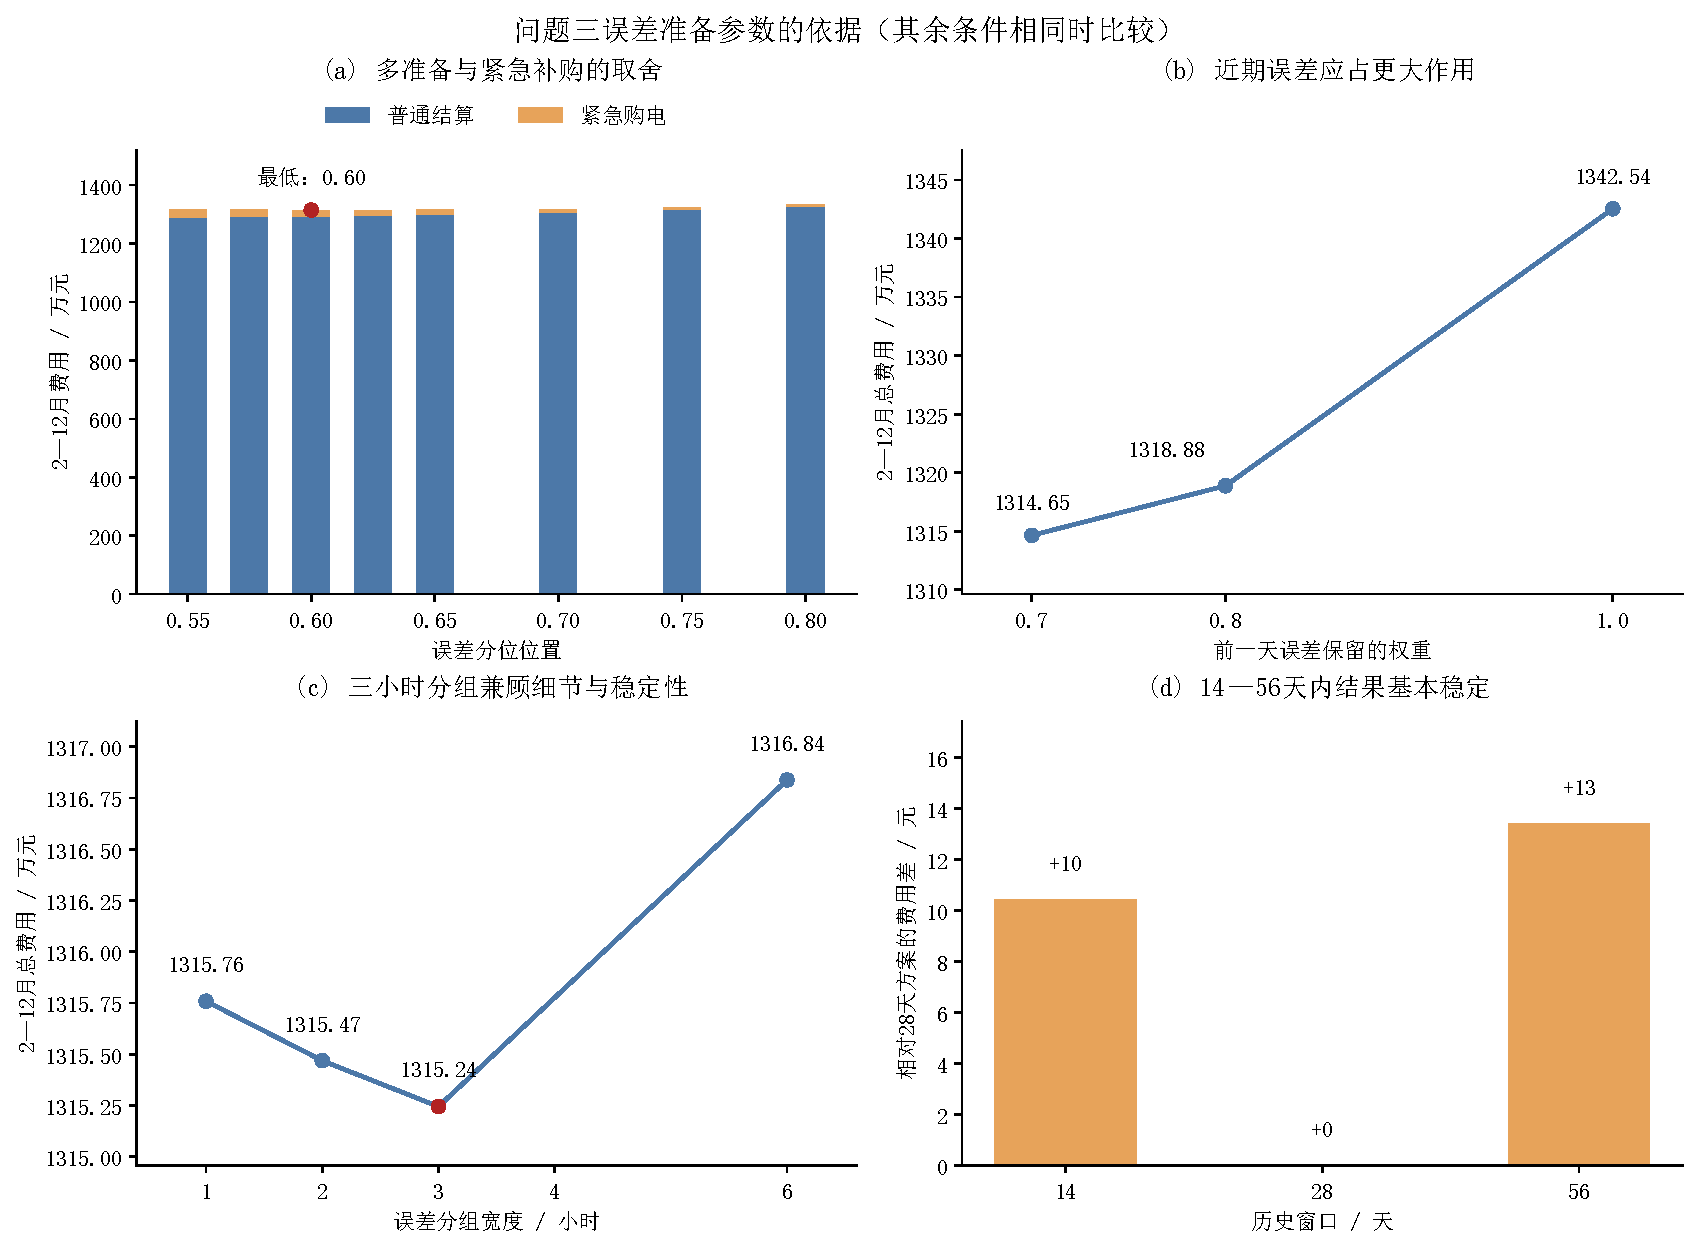
\includegraphics[width=0.95\textwidth]{fig/q3_parameter_interpretability.pdf}
    \caption{近期误差准备参数的费用依据}
    \label{fig:q3_parameter}
\end{figure}

为检验计算结果，对保存的策略重新计算逐10分钟供需、
储电状态、充放电功率、订单锁定和总费用。
费用最大复算误差约为
\[
1.9\times10^{-9}\ \text{元},
\]
各项储能和供电约束均得到满足。

需要说明的是，上述参数是在题目给出的2025年数据范围内比较得到，
能够支持本年度条件下的模型选择与费用分析；
若用于其他年份或其他微网，仍需结合新的运行数据重新校准。

\section{问题四的模型建立与求解}

\subsection{求解思路}

问题四在问题二、三的基础上进一步引入\textbf{实时波动电价}。
此时，每天制定购电计划时，不仅未来负载和光伏未知，未来电价也不能提前获得。
若仍按固定电价安排储能，可能在并不便宜的时段提前充电，或在真正的高价时段到来前过早放电。

因此，我们保留前面已经建立的供需预测、误差准备和储能调度模型，只增加一层\textbf{电价预测}，再利用预测价格重新优化购电。

问题四包含两种运行方式：

\begin{itemize}
    \item \textbf{问题四-2：}每天0:00确定当天订单，日内不能修改；
    \item \textbf{问题四-3：}0:00制定原计划，6:00、12:00和18:00可根据新信息调整未执行订单。
\end{itemize}

由于两种情况下能够获得的信息不同，我们分别采用\textbf{提升树预测零点电价}和\textbf{岭回归更新日内电价}。


\subsection{波动电价预测}

历史数据表明，电价具有较稳定的日内轮廓和周重复特征，但同一时刻在不同日期仍有明显波动。为描述这些变化，价格预测同时使用附件1的日内参考电价、过去四周同星期位置的价格中位数、最近七天同刻中位数和上周同刻价格，并加入预测净负荷、星期位置、年内位置及预测提前时间等信息。

日内分支还利用当天已经发生的价格修正后续判断：以实际价格相对历史同刻基线的偏差描述当天整体偏高或偏低的程度，并利用最近一个区间的偏差反映短时变化。净负荷采用当前能够得到的负载与光伏预测之差，不使用未来实际供需。上述信息构成价格模型的特征向量$\mathbf{x}$。

\subsubsection*{（1）问题四-2：提升树价格预测}

每天0:00尚未获得当天实际价格，因此主要依靠历史价格和供需背景预测。
考虑到这些因素与电价之间可能存在非线性关系，我们采用直方图梯度提升树，其形式为

\begin{equation}
\hat{p}
=
F_0(\mathbf{x})
+
\gamma
\sum_{m=1}^{M}
h_m(\mathbf{x}),
\end{equation}

其中，$M=100$，学习率$\gamma=0.05$，最终每棵树最多包含31个叶节点，每个叶节点至少包含50个训练样本。叶节点数控制模型划分不同价格情形的精细程度；限制每个叶节点的样本量，则避免仅依据少数记录作出过细划分。

\subsubsection*{（2）问题四-3：岭回归价格预测}

在6:00、12:00和18:00，可以利用当天已经发生的实际价格更新后续判断。历史同刻价格、近期价格及当天价格偏差之间具有较强相关性，直接回归可能依靠较大的正负系数相互抵消，使预测对小幅变化过于敏感。为限制这种波动，先按当前训练集的均值和标准差将各特征标准化为$\mathbf{z}_i$，再采用岭回归：

\begin{equation}
\min_{\beta_0,\boldsymbol{\beta}}
\sum_i
\left(
p_i-\beta_0-\mathbf{z}_i^{\mathrm T}\boldsymbol{\beta}
\right)^2
+
\lambda
\sum_j\beta_j^2,
\qquad
\lambda=10.
\end{equation}

目标函数中的第一项衡量价格拟合误差，第二项限制回归系数的大小，截距$\beta_0$不受惩罚。各系数由历史数据拟合，可以为负，也不要求和为1。正则参数$\lambda=10$采用候选比较阶段的固定设置，不将后续残差模型的检验结果作为它的选取依据。为使预测价格保持为正，提升树和岭回归的输出均取不低于0.001元/kWh。

价格模型每7天重新训练一次，使用此前56天内已经兑现的历史样本，历史不足时使用已有记录。构造样本时按原决策时点还原特征，避免将后来才知道的价格和供需写入历史输入。日内各时点更新的是模型输入和预测结果，而不是每天重新训练四次模型。


\subsection{波动电价下的购电模型}

\subsubsection*{（1）问题四-2}

问题四-2直接沿用问题二中的负载、光伏预测、误差准备和储能约束，仅将固定电价替换为0:00预测得到的波动电价。

目标函数为

\begin{equation}
\min J_{4-2}
=
\sum_{t\in T_0}
\hat{p}_{t|0}q_t
-
\nu S_T,
\end{equation}

其中，$q_t$为普通购电量，$S_T$为规划末端储电量。

规划仍延伸至次日24:00，以避免模型在当天末尾过早放空电池，但只固定当天订单。
实际运行中，若普通购电和储能仍无法满足负载，则剩余缺口按照该时段\textbf{实际电价的5倍}进行紧急购电。

\subsubsection*{（2）问题四-3}

问题四-3沿用问题三中的滚动调整模型。设零点原计划为$q_t^0$，当前调整后的订单为$q_t$，则滚动优化目标为

\begin{equation}
\min J_{4-3}
=
\sum_{t\in T_r}
\hat{p}_{t|r}
\left(q_t+5e_t\right)
+
\frac{1}{2}
\sum_{t\in D_r}
\hat{p}_{t|r}
\left|q_t-q_t^0\right|
-
\nu S_T,
\end{equation}

其中，$e_t$为预计紧急购电量，$D_r$表示当前时刻尚未执行的当天时段。

已经执行的订单不再修改；同一时段经过多次调整时，只按照最终订单与零点原计划之间的净变化结算。
预测价格只用于制定购电和储能安排。实际运行结束后，普通购电费、调整费和紧急购电费均按对应供电时段的实际价格结算；未被负载或电池接收的普通订单仍需付款。期末库存的参考价值不作为收入从实际费用中扣除。

供需平衡、储电递推、$1200$--$10800\ \mathrm{kWh}$容量限制、$5000\ \mathrm{kW}$充放电功率限制以及$90\%$充放电效率均沿用问题二、三，不再重复列写。


\subsection{模型求解与方案选择}

给定预测电价后，两条分支均转化为线性规划，并采用HiGHS求解。正式统计范围为2025年2月1日至12月31日，共334天。所有价格候选统一从1月份共同启动过程得到的8592.69 kWh内部储电量开始，在各自分支内保持供需预测、设备参数和实际供电规则一致，以比较价格预测方法对调度费用的影响。

三种价格预测方法的比较结果如表所示。

\begin{table}[H]
    \centering
    \caption{波动电价下不同价格预测模型的比较}
    \small
    \begin{tabular}{ccccc}
        \hline
        分支 & 价格模型 & 价格MAE/(元/kWh) & 总费用/万元 & 紧急购电量/kWh \\
        \hline
        问题四-2 & 历史同刻中位数 & 0.04984 & 1427.22 & 97728.89 \\
        问题四-2 & 岭回归 & 0.04472 & 1426.64 & 99205.19 \\
        问题四-2 & 提升树 & \textbf{0.03884} & \textbf{1425.52} & 98725.98 \\
        \hline
        问题四-3 & 历史同刻中位数 & 0.04676 & 1383.78 & 40144.52 \\
        问题四-3 & 岭回归 & 0.04442 & 1382.29 & \textbf{38733.80} \\
        问题四-3 & 提升树 & \textbf{0.03834} & \textbf{1382.06} & 40116.12 \\
        \hline
    \end{tabular}
\end{table}

表中的提升树采用初始15叶设置。问题四-2中，该方案同时取得最低价格预测误差和最低费用，说明历史因素之间的非线性组合有助于零点价格判断。进一步将每棵树的最大叶节点数由15增加至31后，总费用再减少6605.53元，因此最终采用31叶版本。后文最终费用表对应这一深化后的方案，与候选比较表中的15叶结果有所区别。

问题四-3中，提升树虽然比岭回归少花2273.23元，但仅占总费用约$0.016\%$，同时紧急购电量更多、发生紧急购电的日期也更多。因此，最终选择结构更清楚、紧急购电较少的岭回归方案。


\subsection{最终结果与分析}

两种最终方案的全年结果如下。

\begin{table}[H]
    \centering
    \caption{问题四两种最终方案的全年费用结果}
    \begin{tabular}{lrr}
        \hline
        指标 & 问题四-2 & 问题四-3 \\
        \hline
        普通购电费/元 & 13613522.32 & 13327163.05 \\
        调整费/元 & 0.00 & 268515.82 \\
        紧急购电费/元 & 635048.55 & 227222.48 \\
        \textbf{总费用/元} & \textbf{14248570.87} & \textbf{13822901.35} \\
        紧急购电量/kWh & 98756.33 & 38733.80 \\
        期末内部储电量/kWh & 8692.34 & 7918.81 \\
        \hline
    \end{tabular}
\end{table}

允许日内调整后，虽然增加了约26.85万元的调整费用，但普通购电和紧急购电费用下降更多。因此，问题四-3相较问题四-2共减少费用

\begin{equation}
425669.52\ \text{元},
\end{equation}

约下降

\begin{equation}
2.99\%.
\end{equation}

需要指出的是，这一差值同时包含供需信息更新、价格更新和订单调整等多方面作用，不能全部解释为日内价格更新带来的收益。

为比较两种决策方式在具体日期的运行差异，表~\ref{tab:q4_specified_results}列出题目指定日期的普通订单、紧急购电、日末库存和全天费用。其中，普通订单表示最终需要结算的电量，不等于全部被负载或储能实际接收的电量。

\begin{table}[H]
\centering
\caption{问题四指定日期的购电与储电结果}
\label{tab:q4_specified_results}
\small
\begin{tabular}{llrrrr}
\toprule
分支 & 日期 & 普通订单/kWh & 紧急购电/kWh & 日末库存/kWh & 费用/元 \\
\midrule
问题四-2 & 3月20日  & 62329.63 & 329.13 & 1376.30  & 41909.16 \\
         & 6月21日  & 42375.21 & 0.00   & 10380.22 & 20358.11 \\
         & 9月23日  & 68066.93 & 10.23  & 2592.35  & 44700.97 \\
         & 12月21日 & 94612.77 & 0.00   & 9798.14  & 71357.71 \\
\midrule
问题四-3 & 3月20日  & 61795.52 & 93.27  & 1311.14  & 40921.66 \\
         & 6月21日  & 42176.92 & 14.64  & 10800.00 & 20204.97 \\
         & 9月23日  & 67751.81 & 11.32  & 3463.77  & 45250.33 \\
         & 12月21日 & 93283.52 & 20.53  & 8131.62  & 71876.82 \\
\bottomrule
\end{tabular}
\end{table}

允许日内调整并不保证每个日期的费用都更低。例如，问题四-3在3月20日和6月21日的费用较低，在9月23日和12月21日却较高。两种策略也形成了不同的日末库存，并将差异传递至下一天。因此，指定日期用于解释运行差别，整体优劣仍需结合连续统计期的总费用判断。


\subsection{模型检验}

首先，对保存的订单、供需数据和储电轨迹重新逐段计算。共检查865728个10分钟运行区间，储电递推和全年费用的复算误差均处于浮点计算误差范围内，说明求解结果满足所建立的模型约束。

其次，对价格模型和日内更新机制进行进一步检验，结果如图所示。

\begin{figure}[H]
    \centering
    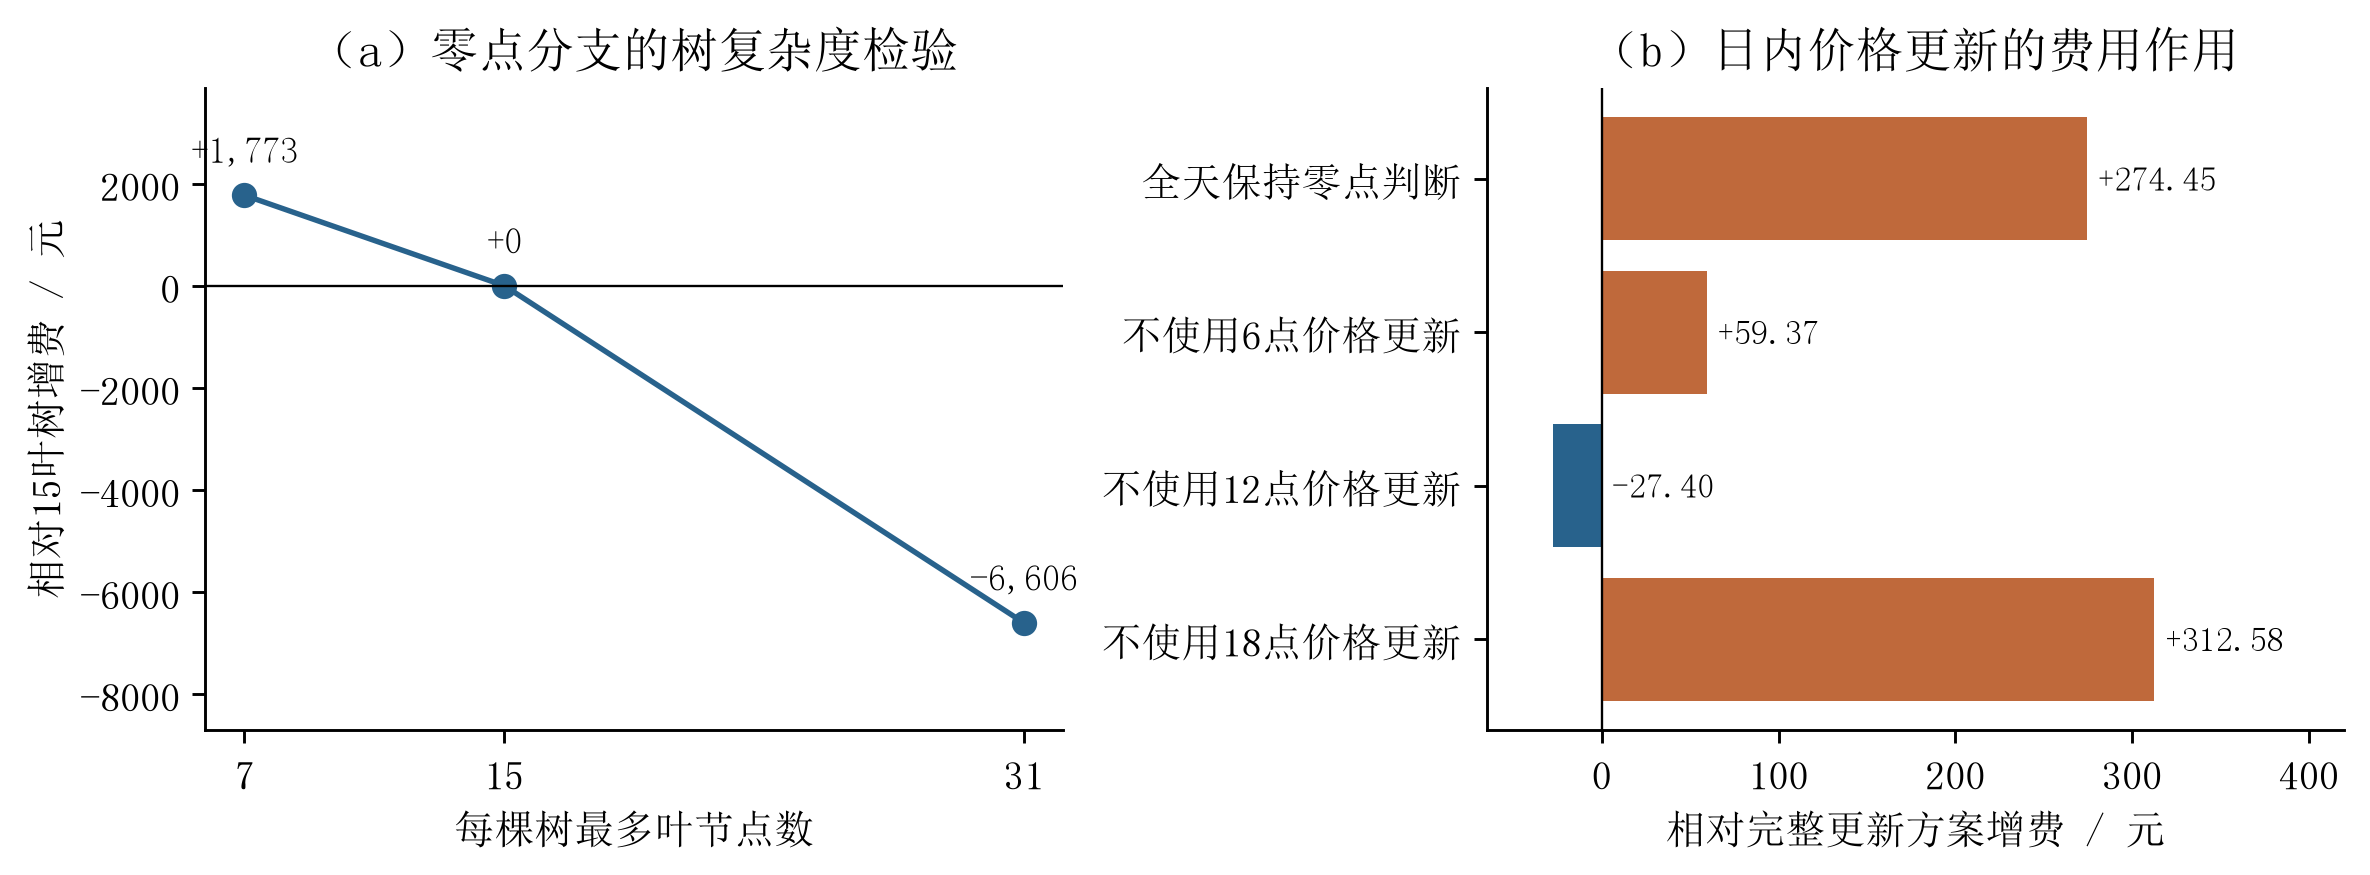
\includegraphics[width=0.95\textwidth]{fig/q4.png}
    \caption{树复杂度与日内价格更新的费用检验}
    \label{fig:q4_model_test}
\end{figure}

\subsubsection*{（1）提升树复杂度检验}

由图\ref{fig:q4_model_test}(a)可见，以15叶模型为基准：

\begin{itemize}
    \item 7叶模型全年费用增加约1773元；
    \item 31叶模型全年费用减少约6606元。
\end{itemize}

因此，在本题比较的三种复杂度下，31叶模型的全年费用最低。不过，该模型仍有部分日期和月份费用高于15叶模型，因此只能说明其在\textbf{本年度总体费用指标下表现更好}。
为排除通过少留期末电量降低费用的影响，进一步按实际价格的第5、第50和第95百分位，对期末最低库存以上的可放电量分别估值。计入剩余电量价值后，31叶方案仍比15叶方案节省5890.24--6423.72元，说明其费用优势并非仅来自期末库存差异。

对于日内分支，还尝试了先确定历史价格基线、再用岭回归预测价格偏差的方式，但所测三档正则强度均未降低费用，因此保留直接预测价格的完整岭回归。

\subsubsection*{（2）日内价格更新检验}

图\ref{fig:q4_model_test}(b)进一步比较不同价格更新方式。以完整的0:00、6:00、12:00和18:00更新方案为基准：

\begin{itemize}
    \item 全天保持零点价格判断，费用增加274.45元；
    \item 不使用6:00价格更新，费用增加59.37元；
    \item 不使用12:00价格更新，费用反而减少27.40元；
    \item 不使用18:00价格更新，费用增加312.58元。
\end{itemize}

结果表明，\textbf{日内价格信息总体具有价值，但并不是每一次更新都一定能够降低费用}。这是因为一次价格更新不仅会改变当前订单，还会改变之后的储电状态，各次更新之间存在相互影响，因此不能将各次费用差简单相加。
在实际价格最高的5\%时段内，问题四-2和问题四-3仍分别发生46086.96 kWh和14665.07 kWh紧急购电。由此可见，储能虽能转移电量，但容量、剩余库存和放电功率仍会限制其缓冲能力，不能完全消除高价与供需偏差叠加时的补购风险。

综上，在波动电价条件下，应先根据当前可获得的历史价格和运行信息预测未来电价，再结合供需预测与储能状态进行统一优化。问题四-2最终采用\textbf{滚动提升树--零点线性规划模型}；问题四-3最终采用\textbf{滚动岭回归--日内调整线性规划模型}。

\section{模型评价与推广}

\subsection{模型优点与创新}

\begin{enumerate}
    \item \textbf{四问共用一套可以核对的电量流骨架。}
    本文始终用十分钟电量连接负载、光伏、外网和电池，并统一处理90\%充电效率、90\%放电效率、储电上下限及功率限制。各问只在信息条件和费用规则发生变化时增加相应模块，避免同一物理过程被重复解释成不同含义。问题一的确定性调度由线性规划完成[1]，后续各问沿用同一基础关系，便于逐段复算。

    \item \textbf{把预测和高价缺口风险分开处理。}
    负载与光伏分别预测，使星期用电规律和近期光伏变化都能被解释[5]；误差准备则专门处理五倍紧急电价造成的损失不对称。候选比较显示，提升树即使改善部分预测误差，也没有超过带近期准备的完整方案。该设计说明模型追求的是最终运行费用和供电可靠性，而不是单一的拟合指标。

    \item \textbf{把日内信息的价值拆成两个可说明的部分。}
    问题三没有把197.28万元的总差额全部归功于新预报，而是先计算日内反馈与改单节省的175.51万元，再计算后发官方预报额外节省的21.78万元。这样可以直接回答题目关于日内预报是否值得引入的问题，也避免把权限变化误写成预测方法的贡献。

    \item \textbf{根据决策方式选择价格模型。}
    问题四没有机械地给两条分支使用同一种算法。零点分支采用提升树表达非线性关系[3]；日内分支采用岭回归稳定处理高度相关的历史价格特征[2]。后者以极小费用差换取更少紧急购电和更清楚的系数含义，体现了经济性、风险和可解释性的综合选择。

    \item \textbf{结论能够追溯到实际运行过程。}
    本文使用SciPy和scikit-learn完成数值计算与候选预测[6,7]，线性规划由HiGHS求解[4]。全年费用均由保存的普通订单、紧急购电和储电轨迹重新计算，并逐段检查供需、库存、功率和结算关系。指定日期的图表进一步说明电池何时补缺、何时达到下限以及为什么仍会发生紧急购电，使模型结论既有总量证据，也有运行过程支撑。
\end{enumerate}


\subsection{模型局限与改进方向}

首先，历史窗口、误差分位、日期衰减和价格模型参数主要在2025年数据内比较。现有结果能够说明本题数据范围内的取舍，但不能证明同一组参数在其他年份或其他地区仍然最优。若获得跨年数据，可按年份滚动回测，并在不同季节分别校准参数，以检验真正的跨年泛化能力。

其次，本文先预测负载、光伏和价格，再把预测结果送入优化。这样的分层结构容易解释，也便于定位误差来源，但没有同时描述三类不确定量可能共同出现的极端情景。后续可构造少量有现实含义的联合情景，比较连续阴天、高负载和高电价叠加时的计划，进一步控制尾部风险。

再次，题目没有提供电池老化费用、外送电价、网络损耗和可中断负载信息，因此本文未把这些因素写入目标函数。若用于真实微网，可增加循环寿命成本、需求响应和售电约束；末端库存的参考价值也应根据下一日市场规则重新估计，而不能直接视为可出售资产。


\subsection{模型推广性评估}

模型的核心输入只有分时负载、本地可再生能源、设备参数、交易价格和允许的决策时点。替换这些数据并重新校准预测与准备参数后，可用于社区、校园、工业园区及偏远地区的微网运行，也可扩展到多台储能、风光互补、充电站和可调负载。滚动求解方式允许系统随着新数据修正未来计划，适合部署在需要持续更新的能源管理平台中。

从社会应用看，该方法优先消纳本地光伏，并通过储能和合理购电减少高峰期对外网的额外压力，有助于提高可再生能源利用率、降低能源浪费，服务碳达峰和碳中和目标[8,9]。推广时还应把安全供电和居民基本用电放在成本优化之前，使节费收益建立在可靠、公平的能源服务之上。这样的应用方向既符合绿色发展和资源节约要求，也体现以人民为中心、共建共享的发展取向。

\end{document}
